%%% master.tex --- 

%%%%%%%%%   Style  %%%%%%%%%%%%%%%%%%%%%%%%%%%%%%%%%%%%%%%%%%%%%%%%%%%%%%%%%%%%%

\documentclass[spanish,a4paper,11pt, openany]{scrbook}

% for images
\usepackage{graphicx} 
% Less detailed TOC
\setcounter{tocdepth}{2}
% for all characters
\usepackage[latin1]{inputenc}
%inline enumeration
\usepackage{paralist}
% to get rid of Underfull \hbox (badness ...) Error message
\usepackage{etoolbox}
%\apptocmd{\thebibliography}{\raggedright}{}{} % this also works but not perfet squared
\apptocmd{\thebibliography}{\hbadness 3503\relax}{}{}
% link outs in PDF
\usepackage{cite} % allows line breaking inside citations
% for url href...
\usepackage{hyperref}
% table color
\usepackage[table]{xcolor}
\rowcolors{1}{white}{lightgray}
% list of abbreviations
\usepackage[intoc]{nomencl}
\makenomenclature
% make caption font tinier
\usepackage[small, bf]{caption}
\setcapindent{10pt}

\usepackage[final]{pdfpages}

%glossary
\usepackage[toc,acronym]{glossaries}
\makeglossaries

%% SPECIAL FUNCTIONS
\newcommand{\myurl}[1] {{\scriptsize \url{#1}}}
\newcommand{\tref}[1] {\hyperref[#1]{Table \ref*{#1}}}
\newcommand{\fref}[2] {\hyperref[#1]{Figure \ref*{#1}#2}}
%\newcommand{\tref}[1] {\hyperref[#1]{Table \ref*{#1} on page \pageref*{#1}}}
%\newcommand{\fref}[2] {\hyperref[#1]{Figure \ref*{#1}#2 on page \pageref*{#1}}}

%%%%%%%%%%%%%%%%%%%%%%%%%%%%%%%%%%%%%%%%%%%%%%%%%%%%%%%%%%%%%%%%%%%%%%%%%%%%%%%%
%%%%%%%%%   Thesis starts here  %%%%%%%%%%%%%%%%%%%%%%%%%%%%%%%%%%%%%%%%%%%%%%%%
%%%%%%%%%%%%%%%%%%%%%%%%%%%%%%%%%%%%%%%%%%%%%%%%%%%%%%%%%%%%%%%%%%%%%%%%%%%%%%%%
 
\begin{document}

\author{Fran�ois Serra}
\title{Modularity and Neutrality in Genomes}
\subtitle{DNA Structure, Components Dynamics and Functionally Related Proteins}
\date{October 2011}
\pagenumbering{alph} % needed to avoid warning message
\maketitle

\newpage

\pagenumbering{roman}

\tableofcontents

\newpage{}
%%% nomenclature.tex --- 

%% Author: francisco@evolution
%% Version: $Id: nomenclature.tex,v 0.0 2011/10/27 13:42:37 francisco Exp$

\printnomenclature[3pt]
\nomenclature{CR}{Complexity Ratio}
\nomenclature{CV}{Complexity Value}
\nomenclature{BWT}{Burros-Wheeler transform}
\nomenclature{MTF}{Move To Front}
\nomenclature{GE}{Genomic Element}
\nomenclature{dN}{Rate of non-synonymous mutations}
\nomenclature{dS}{Rate of synonymous mutations}
\nomenclature{CDS}{DNA coding sequence}
\nomenclature{bp}{DNA base-pair}
\nomenclature{PSG}{Positively selected genes}
\nomenclature{SL}{Significantly Low}
\nomenclature{SH}{Significantly High}
\nomenclature{GSA}{Gene-Set Analysis}
\nomenclature{GSEA}{Gene-Set Enrichment Analysis}
\nomenclature{GSSA}{Gene-Set Selection Analysis}
\nomenclature{RSA}{Relative Species Abundance}
\nomenclature{TE}{Transposable Element}
\nomenclature{UNTB}{Unified Neutral Theory of Biodiversity}
\nomenclature{FDR}{False Discovery Rate}
\nomenclature{chr}{chromosome}
\nomenclature{LRT}{Likelihood Ratio Test}
\nomenclature{H}{Sannon's Entropy}



%%% Local Variables: 
%%% mode: latex
%%% TeX-master: "../master"
%%% End: 

%%% glossary.tex --- 

%% Author: francisco@evolution
%% Version: $Id: glossary.tex,v 0.0 2011/10/27 13:42:37 francisco Exp$

\newglossaryentry{seed}{
  name=seed,
  description={\textit{-sequence} of a gene or a protein, is the sequence used as starting point in the search of homologous sequences within a given set of entries. Extending this concept at genomic level, we can talk about \textit{seed-genome} or \textit{seed-species}. \textbf{\em Note:} In a phylome, it is expected to observe an over-representation of proteins belonging from the seed-species},
  plural=seeds
}

\newglossaryentry{ecological niche}{
  name={Ecological niche},
  description={The role of a species of organisms in an ecological community,defined by the resources that the species requires from its environment. The ''competitive exclusion principle'' implies that species can only stably coexist if they have different ecological niches}
}

\newglossaryentry{optimal foraging theory}{
  name={Optimal Foraging Theory},
  description={A theory that is designed to predict the foraging behaviour that maximizes food intake per unit time}
}

\newglossaryentry{selfish DNA}{
  name=Selfish DNA,
  description={Sequences of DNA that accumulate in the genome through non-selective means, and which have a negative effect on the fitnesses of their hosts}
}

\newglossaryentry{SINE}{
  name=SINE Sequence,
  description={A short interspersed element sequence - this is a \gls{retroposon} sequence of less than 500 bp in length that does not encode the protein activities required for its movement},
  plural=SINES
}

\newglossaryentry{LINE}{
  name=LINE Sequence,
  description={A long interspersed element sequence - typically used for non-long terminal repeat retrotransposons},
  plural=LINES
}

\newglossaryentry{retrotransposon}{
  name=Retrotransposon,
  description={An autonomous transposable element that can move to a new location through an RNA intermediate.Long terminal repeat (LTR) retrotransposons have direct repeats of 300-500 bp ofDNA at each end of the element. These sequences resemble the integrated proviruses of retroviruses. Non-LTR retrotransposons lack LTRs and the organization of their coding sequences is more diverged from that of retroviral sequences}
}

\newglossaryentry{retroposon}{
  name=Retroposon,
  description={A mobile DNA sequence that can move to new locations through an RNA intermediate}
}

\newglossaryentry{transposon}{
  name=transposon,
  description={A mobile DNA sequence that moves to new genomic locations through a DNA route, rather than through an RNA intermediate. This movement is catalysed by the action of a transposase protein that is encoded by an autonomous element}
}

\newglossaryentry{trophic}{
  name=trophic,
  description={Of or involving the feeding habits or food relationship of different organisms in a food chain}
}

%%% Local Variables: 
%%% mode: latex
%%% TeX-master: "../master"
%%% End: 

\newpage{}



%%%%%%%%%   Style  %%%%%%%%%%%%%%%%%%%%%%%%%%%%%%%%%%%%%%%%%%%%%%%%%%%%%%%%%%%%%

\documentclass[spanish,a4paper,11pt, openany]{scrbook}
% \documentclass[spanish,a4paper,11pt, openany]{afthesis}
% \documentclass[spanish]{hepthesis}
% \documentclass[spanish]{muthesis}
% \documentclass[spanish]{usthesis}


% for images
\usepackage{graphicx} 
 % Less detailed TOC
\setcounter{tocdepth}{3}   
% link outs in PDF
\usepackage{hyperref}
% for all characters
\usepackage[latin1]{inputenc}

%inline enumeration
\usepackage{paralist}

% list of abbreviations
\usepackage{nomencl}
\makenomenclature

%% Aesthetic spacing redefines that look nicer to me than the defaults.
% \setlength{\cftbeforepartskip}{1.5ex}
% \setlength{\cftbeforechapskip}{2.5ex}
% \setlength{\cftbeforesecskip}{0.5ex}

% German style of paragraph formatting, i.e. no indents.
% \setlength{\parskip}{1.3ex plus 0.2ex minus 0.2ex}
% \setlength{\parindent}{0pt}


% some layout    
%\usepackage{geometry}
%\geometry{tmargin=2.2cm,bmargin=2.4cm}


%%%%%%%%%%%%%%%%%%%%%%%%%%%%%%%%%%%%%%%%%%%%%%%%%%%%%%%%%%%%%%%%%%%%%%%%%%%%%%%%
%%%%%%%%%   Thesis starts here  %%%%%%%%%%%%%%%%%%%%%%%%%%%%%%%%%%%%%%%%%%%%%%%%
%%%%%%%%%%%%%%%%%%%%%%%%%%%%%%%%%%%%%%%%%%%%%%%%%%%%%%%%%%%%%%%%%%%%%%%%%%%%%%%%

\begin{document}
% \pagestyle{empty}
\author{Fran�ois Serra}
\title{Adaptation in genes, duplicates, families, functional
  modules and genomes}
\date{October 2011}
\pagenumbering{alph} % needed to avoid warning message
\maketitle


\newpage

\pagenumbering{roman}

\tableofcontents

\newpage{}

\printnomenclature[3]
\nomenclature{CR}{Complexity Ratio}
\nomenclature{BWT}{Burros-Wheeler transform}

\pagenumbering{arabic}

\chapter{Introduction}
\label{intro}
%%% introduction.tex --- 

%% Author: garamonfok@gros
%% Version: $Id: introduction.tex,v 0.0 2011/10/09 18:39:32 garamonfok Exp$

\section{What is DNA? How genes rose?}
\section{Definition of neutrality}
\subsection{Neutrality in modularity}

Explanation of protein networks by to parameters probability of edge deletion $\delta$ and probability of link creation $\alpha$ after a single gene duplication \cite{Sole2008}

\section{Life in DNA, from genes to repetitive elements.}
\section{Adaptive changes to evolutionary speed}
\section{Evolution, and the detection at molecular level}
\section{Grouping genes and finding evolutionary patterns}


%%% Local Variables: 
%%% mode: latex
%%% TeX-master: "../../master"
%%% End: 


\part{Structure and dynamics of genomes}
\chapter{Random-like structure of DNA}
\label{chap:dna_struct}
%%% dna_struct.tex --- 


\section{Background}
\label{sec:dna_struct-intro}

From a biological perspective it seems obvious that DNA is something else than random mix of A, T, G and C nucleotides. Genomes are composed of functional elements as can be protein-coding genes, or promoters but also by non-functional elements like repetitive elements that by definition can not be random when taken together. However to what extent can we state that genomes are not a random soup of 4 letters? From the first analysis of the human genome \cite{Lander2001} we have some idea of the proportion of each of the \textit{families} of elements \fref{fig:prop_rep}{}. Intuitively we could assume that the structure of DNA is different in those families of genomic elements (GE). The sequence of a protein-coding gene would represent a specific selection of nucleotides with surely the highest informational content, while introns would tend more to random assembly and finally we can easily imagine that simple repeats present some biases towards 2 or 3 nucleotides (e.g.: CpG islands).

\begin{figure}[htpb] 
\centering 
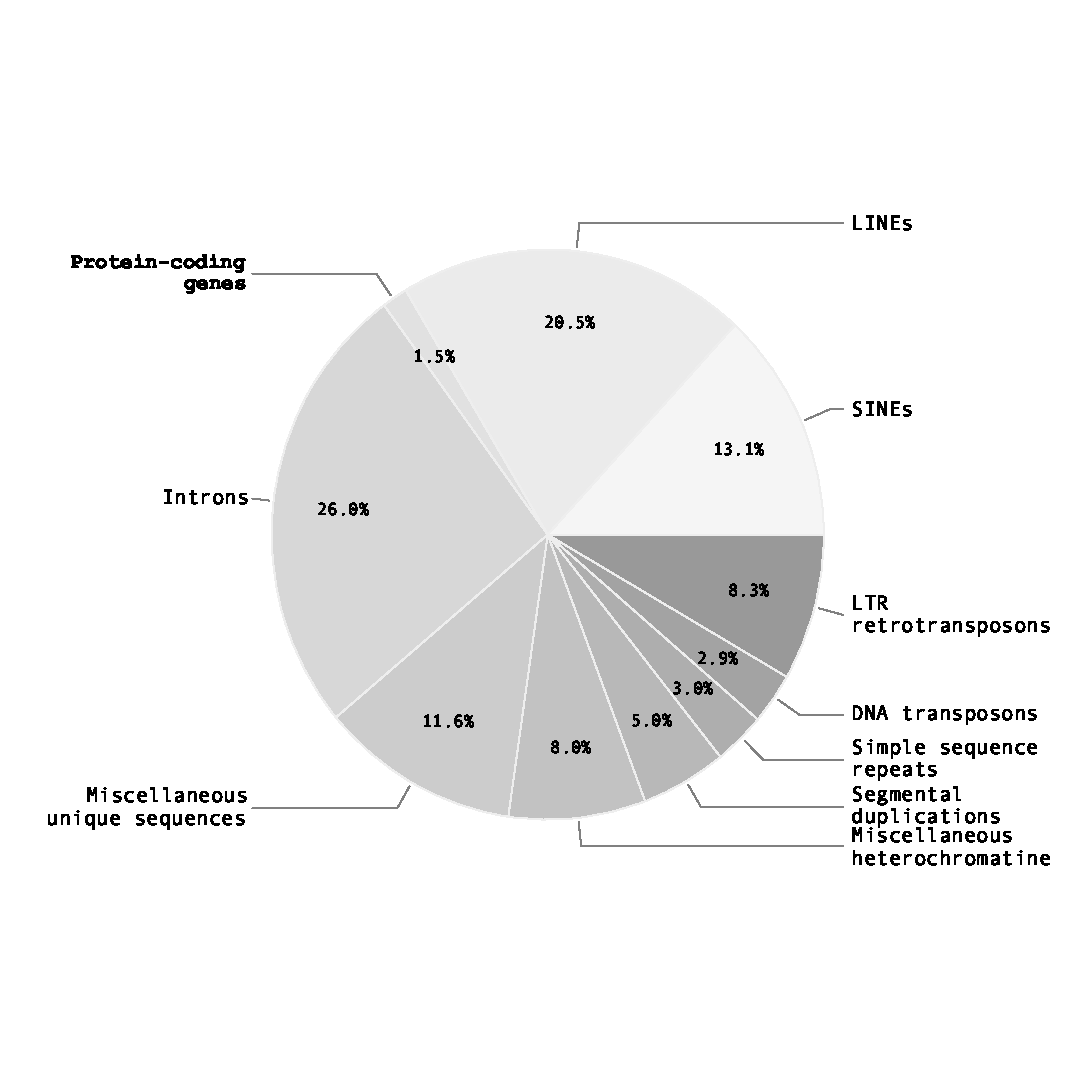
\includegraphics[trim=0cm 3cm 0cm 3cm, width=\textwidth]{tex_source/figures/dna_struct/prop_rep.pdf}
\caption[Genomic components of human genome]{{\bf Genomic components of human genome.}\\
Proportion of the major families of different genomic elements (GE) in the human genome according to \cite{Lander2001}}
\label{fig:prop_rep}
\end{figure}



\cite{Gregory2005}

This question could be solved in some sense by measuring genomes entropy. This measure presents the disadvantage that extreme cases of high entropy could correspond to \begin{inparaenum}[\itshape a\upshape)] \item {\bf a specially high content of information}, entropy-based algorithms are actually used to predict or confirm automatic detection of genes \cite{Du2006,Gerstein2007}, \item {\bf an exact random structure}, some work in the sense of testing the random structure of DNA have been done using entropy \cite{Loewenstern1999}. \end{inparaenum} However this characteristic of entropy could be only a semantic problem if we use it as a measure of relative variation in DNA complexity in genomes, and try to discern statistical patterns in the DNA sequences of different genomic element such as interspersed repeats or functional element (like protein-coding genes). This kind of description of 1DNA sequence complexity was already done by \cite{Holste2001}, but only in human chromosome 22.

\section{Results and Discussion}
\label{sec:dna_struct-result}

\subsection{Computing genome complexity}
\label{sec:comp-genome-compl}


Complexity value (CV) of complete genomes of 54 species of 20 major systematic groups of organisms, ranging 3.4Gb to 1.6Kb genome size was computed \tref{tab:genome}. The distribution of these complexity values showed an accurate fit to a linear regression model when genome size was used as the independent variable, with p $<$ 2.0e-16, \fref{fig:gen_compl}{-A}. The slope (alpha) of the regression (alpha=0.967), was very close to the maximum complexity slope (alpha = 1). Residual variation around the fitted regression was almost null (adjusted-R2 = 0.987). The fit of genomes to almost maximum complexity slope is remarkable considering that the linear model covers six order of magnitude of genome size along all diversity of life. From the shortest single-strand RNA genome of \textit{Hepatitis D} virus (size $\sim$ 1.69e+03 bp) to the largest double-strand DNA genome of the short-tailed opossum (size $\sim$ 3.41e+09 bp). Obligate endosymbionts bacteria with extreme reduction of genome size (\textit{Carsonella ruddii}, \textit{Buchnera aphidicola}, and \textit{Ureaplasma urealyticum}) \cite{Wernegreen2002}; parthenogenetic crustaceans with ubiquitous duplications of genes (\textit{Daphnia pulex}), archean organisms living in extreme environmental conditions (\textit{Sulfolobus islandicus}, \textit{Methanocaldococcus vulcanius}, \textit{Thermococcus sibiricus}), eukaryotes with a variable number of repetitive families, as well as the first synthetic organism made by humans (\textit{Synthetic mycoplasma mycoides}) \cite{Gibson2010}, fit the slope of the linear regression model. 

\begin{FPtable}
\raggedright
\resizebox{418pt}{!}{%
  \begin{tabular}{ l l p{62pt} l r r r r }
  \hline
  \textbf{Features} & \textbf{Species} & \textbf{ACN-EV} &
  \textbf{Clade} & \multicolumn{1}{l}{\textbf{GS}} &
  \multicolumn{1}{l}{\textbf{GC}} & \multicolumn{1}{l}{\textbf{GCR}} &
  \multicolumn{1}{l}{\textbf{Dmax}} \\ \hline
RNA & Hepatitis B & NC3977.1 & Virus & 1,682 & 1,671 & 1 & 0 \\
SGS-RNA & Hepatitis D & D01075.1 & Virus & 3,215 & 3,210 & 0.9984 & 0.0016 \\
SSD & Tomato mosaic & NC010836 \& NC10835.1 & Virus & 5,058 & 5,040 & 0.9964 & 0.0036 \\
SSD & Enterobacteria phage m13 & V00604 & Phage & 6,407 & 6,367 & 0.9938 & 0.0062 \\
RNA & HIV 1 & NC001802 & Virus & 9,181 & 9,105 & 0.9917 & 0.0083 \\
RNA & Sudan ebolavirus & NC006432 & Virus & 18,875 & 18,842 & 0.9983 & 0.0017 \\
DSD & Enterobacteria phage lambda & NC001416 & Phage & 48,502 & 48,381 & 0.9975 & 0.0025 \\
DSD & Human herpesvirus1 & NC001806 & Virus & 152,261 & 150,036 & 0.9854 & 0.0146 \\
SBG-IP-RG & Carsonella ruddii & NC008512  & Bacteria & 159,662 & 146,930 & 0.9203 & 0.0797 \\
IP-RG & Buchnera aphidicola & AE013218.1 & Bacteria & 642,122 & 626,533 & 0.9757 & 0.0243 \\
IP-RG & Ureaplasma urealyticum & CP001184 & Bacteria & 873,755 & 840,812 & 0.9623 & 0.0377 \\
SL & Synthetic mycoplasma mycoides & CP002027.1 & Bacteria & 1,078,809 & 1,026,444 & 0.9515 & 0.0485 \\
EE & Thermococcus sibiricus & CP001463.1 & Archaea & 1,242,891 & 1,237,320 & 0.9955 & 0.0045 \\
EE & Methanocaldococcus vulcanius & CP001787.1 & Archaea & 1,746,040 & 1,708,968 & 0.9788 & 0.0212 \\
EE & Sulfolobus islandicus & CP001731.1 & Archaea & 2,722,004 & 2,692,455 & 0.9891 & 0.0109 \\
 & Bacillus subtilis & {\it E!} Bacteria 9 & Bacteria & 4,215,606 & 4,198,057 & 0.9958 & 0.0042 \\
 & Mycobacterium tuberculosis & {\it E!} Bacteria 9 & Bacteria & 4,411,532 & 4,348,606 & 0.9857 & 0.0143 \\
 & Escherichia coli & CP001396.1 & Bacteria & 4,578,159 & 4,551,258 & 0.9941 & 0.0059 \\
LBG & Burkholderia xenovorans & NC007951-3 & Bacteria & 9,731,138 & 9,593,486 & 0.9859 & 0.0141 \\
AP & Saccharomyces cerevisiae & {\it E!} Fungi 3 & Fungi & 12,070,898 & 11,974,342 & 0.992 & 0.008 \\
UE & Plasmodium falciparum & {\it E!} Protists 9 & Apicomplexa & 23,263,332 & 21,070,640 & 0.9057 & 0.0943 \\
UE & Phaeodactylum tricornutum & {\it E!} Protists 9 & Heterokonta & 25,805,651 & 25,667,448 & 0.9946 & 0.0054 \\
UE & Dictyostelium discoideum & {\it E!} Protists 9 & Amebozoa & 31,199,234 & 31,023,020 & 0.9944 & 0.0056 \\
UE & Thalassiosira pseudonana & {\it E!} Protists 9 & Heterokonta & 33,919,934 & 30,877,496 & 0.9103 & 0.0897 \\
 & Ciona intestinalis & {\it E!} 62 & Urochordate & 87,649,861 & 84,674,396 & 0.9661 & 0.0339 \\
 & Caenorhabditis elegans & {\it E!} Metazoa 9 & Invertebrates & 100,272,217 & 97,720,472 & 0.9746 & 0.0254 \\
 & Tribolium castaneum & -1- & Invertebrates & 112,129,668 & 109,424,212 & 0.9759 & 0.0241 \\
AP-RG & Arabidopsis thaliana & {\it E!} Plants 9 & Plants & 118,960,082 & 116,563,556 & 0.9799 & 0.0201 \\
 & Drosophila melanogaster & {\it E!} Metazoa 9 & Invertebrates & 120,290,887 & 118,973,632 & 0.989 & 0.011 \\
GE & Daphnia pulex & {\it E!} Metazoa 9 & Invertebrates & 158,632,523 & 150,111,316 & 0.9463 & 0.0537 \\
AP & Arabidopsis lyrata & {\it E!} Plants 9 & Plants & 173,245,910 & 161,798,504 & 0.9339 & 0.0661 \\
AP & Tetraodon nigroviridis & {\it E!} 62 & Fishes & 208,708,313 & 207,067,712 & 0.9921 & 0.0079 \\
 & Apis mellifera & {\it E!} Metazoa 9 & Invertebrates & 224,750,524 & 219,278,732 & 0.9757 & 0.0243 \\
 & Anopheles gambiae & {\it E!} Metazoa 9 & Invertebrates & 225,028,531 & 221,180,624 & 0.9829 & 0.0171 \\
AP & Brachypodium distachyon & {\it E!} Plants 9 & Plants & 270,058,956 & 257,893,524 & 0.955 & 0.045 \\
AP & Oryza sativa & {\it E!} Plants 9 & Plants & 293,104,375 & 271,137,108 & 0.9251 & 0.0749 \\
AP & Populus trichocarpa & {\it E!} Plants 9 & Plants & 370,421,283 & 352,063,876 & 0.9504 & 0.0496 \\
AP & Physcomitrella patens & {\it E!} Plants 9 & Bryophyta & 453,927,385 & 399,508,556 & 0.8801 & 0.1199 \\
AP & Sorghum bicolor & {\it E!} Plants 9 & Plants & 625,636,188 & 491,993,216 & 0.7864 & 0.2136 \\
AP & Oryzias latipes & {\it E!} 62 & Fishes & 582,126,393 & 562,662,192 & 0.9666 & 0.0334 \\
 & Gallus gallus & {\it E!} 62 & Birds & 984,855,151 & 971,359,304 & 0.9863 & 0.0137 \\
 & Taeniopygia guttata & {\it E!} 62 & Birds & 1,013,982,659 & 996,918,996 & 0.9832 & 0.0168 \\
AP & Danio rerio & {\it E!} 62 & Fishes & 1,354,636,069 & 1,191,452,752 & 0.8795 & 0.1205 \\
AP-RP & Zea mays & {\it E!} Plants 9 & Plants & 2,045,697,632 & 1,197,255,904 & 0.5853 & 0.4147 \\
 & Canis familiaris & {\it E!} 62 & Mammals & 2,309,875,279 & 2,272,374,188 & 0.9838 & 0.0162 \\
 & Equus caballus & {\it E!} 62 & Mammals & 2,335,454,424 & 2,307,202,104 & 0.9879 & 0.0121 \\
 & Bos taurus & {\it E!} 62 & Mammals & 2,466,956,401 & 2,406,743,280 & 0.9756 & 0.0244 \\
 & Rattus norvegicus & {\it E!} 62 & Mammals & 2,477,053,718 & 2,430,894,052 & 0.9814 & 0.0186 \\
 & Mus musculus & {\it E!} 62 & Mammals & 2,558,509,481 & 2,521,038,616 & 0.9854 & 0.0146 \\
 & Pan troglodytes & {\it E!} 62 & Mammals & 2,598,733,311 & 2,566,544,200 & 0.9876 & 0.0124 \\
 & Macaca mulatta & {\it E!} 62 & Mammals & 2,646,263,164 & 2,621,196,144 & 0.9905 & 0.0095 \\
 & Pongo abelii & {\it E!} 62 & Mammals & 2,722,968,487 & 2,697,592,876 & 0.9907 & 0.0093 \\
 & Homo sapiens & {\it E!} 62 & Mammals & 2,858,658,095 &
 2,841,049,052 & 0.9938 & 0.0062 \\
LGS & Monodelphis domestica & {\it E!} 62 & Mammals & 3,412,593,369 & 3,402,944,248 & 0.9972 & 0.0028 \\ \hline
  \end{tabular}
}
\caption[Genomes Complexity.]%
{{\bf Genomes Complexity.} \\Genomes size (GS), genomes complexity (GC), genome complexity ratio ($GCR=\frac{GC}{GS}$), and deviation from the maximum GCR (Dmax=1-GCV) for 54 species of different taxa. NCBI accession number or Ensembl ({\it E!}) version (ACN-EV). {\bf \em Features}: {\bf AP}: Ancient Polyploid; {\bf DSD}: Double-Strand DNA; {\bf EE}: Extreme Environment; {\bf GE}: Gene Expansion; {\bf IP}: Intracellular Parasite; {\bf LBG}: Largest Bacterial Genome; {\bf LGS}: Largest Genome Sequenced; {\bf RG}: Reduced Genome; {\bf RNA}: RNA Virus; {\bf RP}: Recent Polyploid; {\bf SBG}: Shortest Bacterial Genome; {\bf SGS}: Shortest Genome Sequenced; {\bf SL}: Synthetic Life; {\bf SSD}: Single-Strand DNA; {\bf UE}: Unicellular Eukaryote. {\bf \em Notes}: -1-: \myurl{http://www.hgsc.bcm.tmc.edu/ftp-archive/Tcastaneum/Tcas3.0/}
}
\label{tab:genome}
\end{FPtable}


\begin{FPfigure}
\centering 
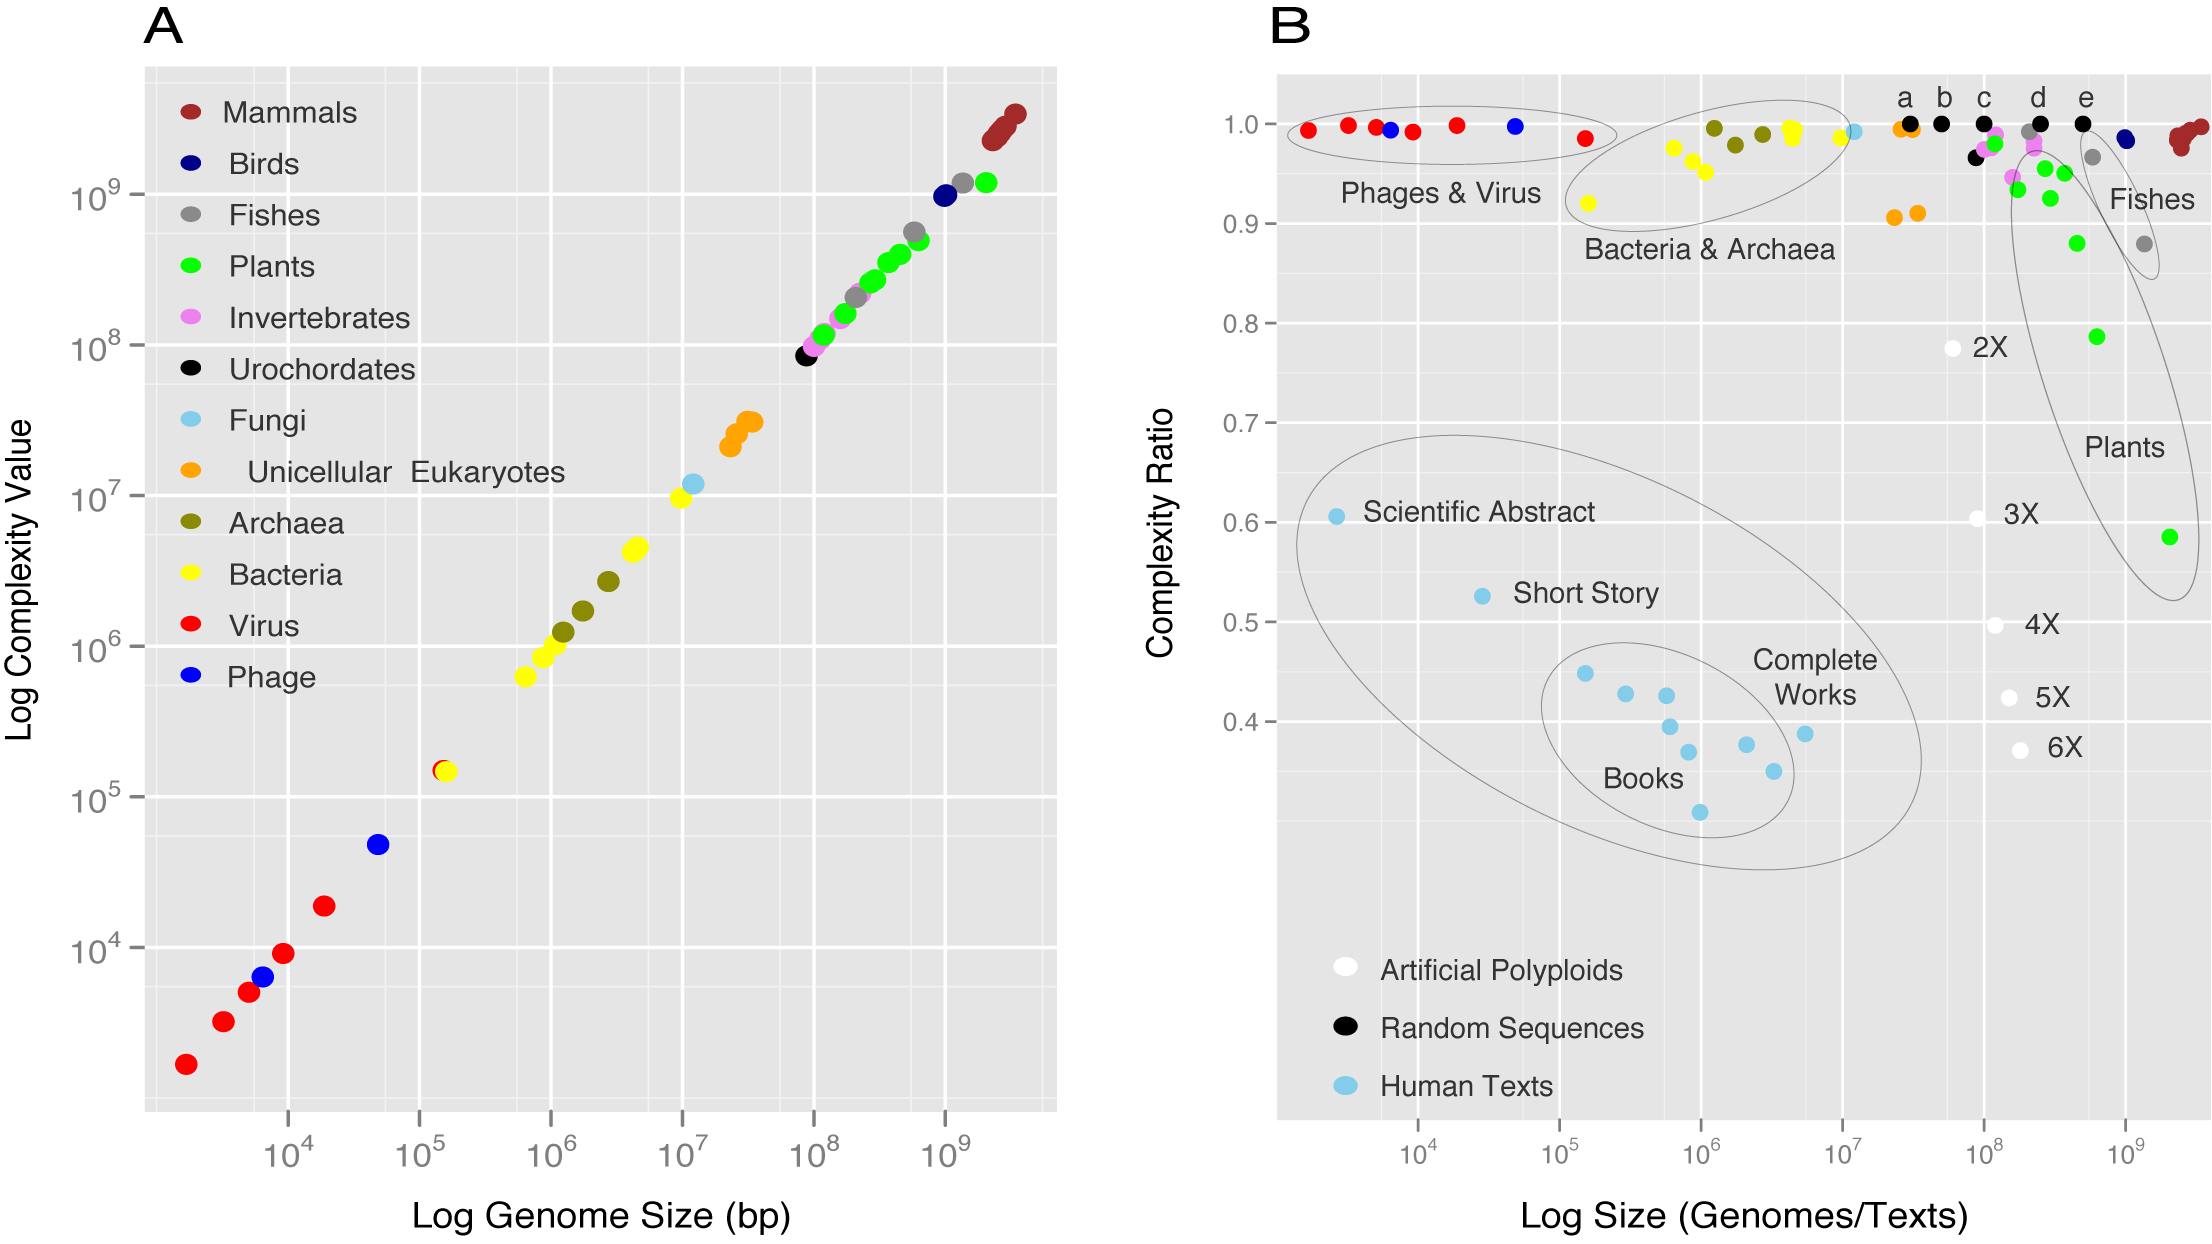
\includegraphics[width=\textwidth]{tex_source/figures/dna_struct/genome_complexity.png}
\caption[Genome complexity value]{{\bf Genome complexity value.} \\\textbf{(A)} Complexity values and genome size of 54 genomes. Log scales are used to display species diversity. Species listed by genome size increase are (see \tref{tab:genome} for details): \textit{Hepatitis D} (V), \textit{Hepatitis B} (V), \textit{Tomato mosaic} (V), \textit{Enterobacteria phage m13} (Ph), \textit{Hiv 1} (V), \textit{Sudan ebolavirus} (V), \textit{Enterobacteria phage lambda} (Ph), \textit{Human herpesvirus1} (V), \textit{Carsonella ruddii} (Ba), \textit{Buchnera aphidicola} (Ba), \textit{Ureaplasma urealyticum} (Ba), \textit{Synthetic mycoplasma mycoides} (Ba), \textit{Thermococcus sibiricus} (Ar), \textit{Methanocaldococcus vulcanius} (Ar), \textit{Sulfolobus islandicus} (Ar), \textit{Bacillus subtilis} (Ba), \textit{Mycobacterium tuberculosis} (Ba), \textit{Escherichia coli} (Ba), \textit{Burkholderia xenovorans} (Ba), \textit{Saccharomyces cerevisiae} (Fu), \textit{Plasmodium falciparum} (Ue), \textit{Phaeodactylum tricornutum} (Ue), \textit{Thalassiosira pseudonana} (Ue), \textit{Dictyostelium discoideum} (Ue), \textit{Ciona intestinalis} (Ur), \textit{Caenorhabditis elegans} (I), \textit{Tribolium castaneum} (I), \textit{Arabidopsis thaliana} (Pl), \textit{Drosophila melanogaster} (I), \textit{Daphnia pulex} (I), \textit{Arabidopsis lyrata} (Pl), \textit{Tetraodon nigroviridis} (Fi), \textit{Apis mellifera} (I), \textit{Anopheles gambiae} (I), \textit{Brachypodium distachyon} (Pl), \textit{Oryza sativa} (Pl), \textit{Populus trichocarpa} (Pl), \textit{Physcomitrella patens} (Pl), \textit{Oryzias latipes} (Fi), \textit{Sorghum bicolor} (Pl), \textit{Gallus gallus} (Bi), \textit{Taeniopygia guttata} (Bi), \textit{Danio rerio} (Fi), \textit{Zea mays} (Pl), \textit{Canis familiaris} (M), \textit{Equus caballus} (M), \textit{Bos taurus} (M), \textit{Rattus norvegicus} (M), \textit{Mus musculus} (M), \textit{Pan troglodytes} (M), \textit{Macaca mulatta} (M), \textit{Pongo abelii} (M), \textit{Homo sapiens} (M), \textit{Monodelphis domestica} (M). V: Virus, Ph: Phage, Ba: Bacteria, A: Archaea, Fu: Fungi, Ue: Unicellular eukaryote, Ur: Urochordate, I: Invertebrate, Pl: Plants, Fi: Fish, Bi: Bird, M: Mammal. \textbf{(B)} Most genomes have complexity ratio (CR) between 0.90 and 1.0. Four polyploid species have CR $<$ 0.9: P. patens (0.880), \textit{D. rerio} (0.879), \textit{S. bicolor} (0.786) and \textit{Z. mays} (0.585). a, b, c, d, e correspond to random [ACGT] strings of 30, 50, 100, 250 and 500 Mb length, respectively. 2$\times$ to 6$\times$ correspond to random polyploids [ACGT] sequences where 1$\times$ is ``a''. Changes in sequence length due to polyploidy produce no change in complexity ratio (see \tref{tab:book_compl}). Notice the low CR of human texts (see Table S3 for details). }
\label{fig:gen_compl}
\end{FPfigure}

We studied deviations of complexity value to the slope (alpha) by computing the complexity ratio (CR), and the deviation to the maximum ratio (Dmax = 1- CR). According to \tref{tab:genome}, only ten species showed Dmax $>$ 0.05. These are: six ancient or recent polyploid species; the most extreme case of genome reduction in bacteria; the explosive case of gene expansion in Daphnia, and two unicellular eukaryotes.

The highest CR=1 was obtained for non-polyploid (1$\times$), randomly generated sequences with uniform distribution of ACGT; however, CR falls exponentially when ploidy level increases reaching CR=0.25 for 10$\times$ \tref{tab:book_compl}. Differences in CR were calculated for polyploids after log transformation and linear regression model adjustment, providing a slope (alpha) = -0.81 (adjusted-R2 = 0.97, p $<<$ 0.0001). 

\begin{table}[htbp]
\resizebox{418pt}{!}{%
\begin{tabular}{ l l l r r r }
\hline
\textbf{Features} & \textbf{Author - Writings} & \textbf{Language} & \multicolumn{1}{l}{\textbf{L}} & \multicolumn{1}{l}{\textbf{C}} & \multicolumn{1}{l}{\textbf{CR}} \\ \hline
SA & C. Venter. The human genome (abstract) & English & 2,662 & 1,613 & 0.6059 \\
SS & J. L. Borges. El Aleph & Spanish & 28,507 & 14,991 & 0.5259 \\
B & A. Von Goethe. Torcuato Tasso & German & 152,104 & 68,187 & 0.4483 \\
B & H. Quiroga. Cuentos amor, locura y muerte & Spanish & 293,482 & 125,552 & 0.4278 \\
B & D. F. Sarmiento. Facundo & Spanish & 601,477 & 242,982 & 0.4259 \\
B & D. Alighieri. Divina Commedia & Italian & 570,480 & 301,609 & 0.3692 \\
B & I. Newton. Principia Mathematica & Latin & 817,032 & 237,558 & 0.395 \\
B & B C. Darwin. The Origin of species & English & 981,958 & 303,503 & 0.3091 \\
B & B M. Cervantes. El Quijote & Spanish & 2,097,943 & 790,702 & 0.3769 \\
B & B V. Hugo. Les Miserables & French & 3,259,269 & 1,141,378 & 0.3502 \\
CW & W. Shakespeare & English & 5,447,165 & 2,111,425 & 0.3876 \\ \hline
\end{tabular}
}
\caption[Human language Complexity]{\textbf{Human language Complexity}\\
Work length (L), complexity (C), complexity ratio (CR), and deviations from the maximum ratio of complexity (Dmax=1- CR) for 11 human writings in six different languages. Features: SA: Scientific abstract, SS: Short story; B: Book, CW: Complete Work
}
\label{tab:book_compl}
\end{table}

Complexity ratios of complete genomes, random sequences of different ploidy and human language texts are displayed in \fref{fig:gen_compl}{-B}. Maximum CR corresponds to random sequence of lengths ranging from 5 Kb to 2.5 Gb (a, b, c, d and e). Non-polyploid genomes showed CR $>$ 0.90. Within polyploids the lowest ratio corresponds to \textit{Z. mays} with CR=0.58, and the next to the lowest ratio, its closest relative \textit{S. bicolor} with CR=0.78. Overall strings analyzed, the lowest CR was obtained in human language texts. CR of 11 human texts of different sizes and languages, from short scientific abstract to the complete works of William Shakespeare, are also depicted \fref{fig:gen_compl}{-B} and \fref{fig:lang_compl}{}. CR diminishes as texts size increases, due to the limited lexicon and the fixed language grammar. Complexity reached the lowest ratio in Darwin's Origin of Species (~ 0.309), which is comparable to the CR of a random polyploid sequence of ~ 7$\times$. Observe that text sizes are contained in the range of phages, virus and bacteria genome sizes. Details of complexities of human writings are in shown \tref{tab:book_compl}.

\begin{figure}[htpb] 
\centering
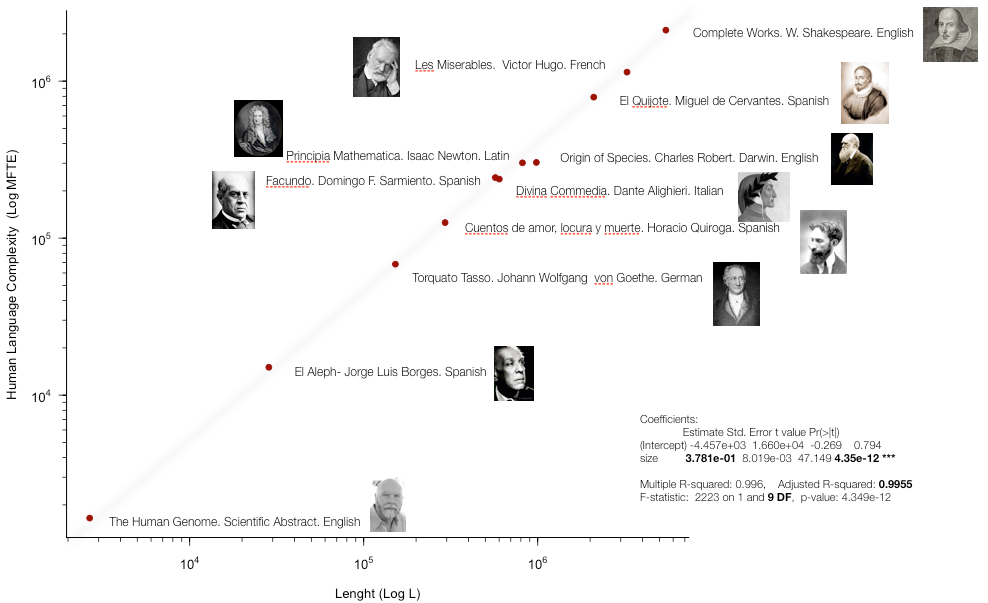
\includegraphics[width=\textwidth]{tex_source/figures/dna_struct/language_complexity.png}
\caption[Human language complexity]{{\bf Human language complexity.} \\
Complexity in human writings shows a constant increase with text length. Regression analysis shows that in contrast to genomes, human language is highly repetitive. While genomes match an almost perfect regression of slope ~1, human language complexity fits a linear regression model with slope alpha=0.378, (adjusted R = 0.995).}
\label{fig:lang_compl}
\end{figure}

\subsection{Genome complexity and ploidy level}
\label{sec:genome-compl-ploidy}

Recent polyploid species as maize and sorghum exhibited noticeably low complexity ratios, however, ancient polyploids and non-polyploids had indistinguishable complexity ratios. We tested the hypothesis that the observed genome complexity values are correlated with size and ploidy level. A categorical variable divided polyploid (ancient or recent), and non-polyploid species described in \tref{tab:genome}. The size-interaction term provided significant deviations (p $<$ 2e-16, adjusted-R2 = 0.997), while independent linear models slopes were 0.633 (p $<$ 4.8e-07, adjusted-R2 = 0.921), and 0.988 (p $<$ 2e-16, adjusted-R2 = 1.00) for polyploid and non-polyploid genomes. 

\subsection{Chromosome complexity}
\label{sec:chrom-compl}

Complexity value of each eukaryote chromosome (567 autosomes of 31 species) was computed and plotted against size \fref{fig:chr_compl}{-A}. Linear regression models considering the full dataset, or excluding polyploid species revealed a very significant statistical relationship (slope = 0.924, adjusted-R2 = 0.989, p $<$ 2e-16, or slope = 0.951, adjusted-R2 = 0.999, p $<$ 2e- 16, respectively). The adjustment of a linear regression model to chromosomes of polyploid species was statistically significant (p $<$ 2e-16, R2 = 0.982), while their complexity values exhibited a lower slope (alpha= 0.696), than the complexity values of chromosomes of non- polyploid species. Again, as was observed in genomes, the size-interaction term was statistically significant (p $<$ 2e-16), suggesting that complexity and size deviates differently for chromosomes of polyploid and non-polyploid species. Notice that for non-polyploid species the slope of their chromosome complexity values against size almost coincides with the slope of their genome complexity values (alpha = 0.989, 0.988, respectively). \fref{fig:chr_compl}{-B} displays CR for chromosomes. The boxplot inside shows the distribution of CR for all chromosomes. The fist quartile of the full sample indicates that 75\% of the data are above 0.958, while the median and mean was 0.974 and 0.964. The minimum CR value corresponds to maize chromosome 10 (0.683), and maximum to \textit{P. tricornutum} chromosome 28 (0.999). Opossum chromosome 1 (the largest chromosome) has a CR of 0.942. Mean CR of maize's chromosomes was 0.698, while maize genome CR was 0.585. The difference suggests extensive duplicated regions in maize chromosomes, which was previously described in \cite{Weber1989,Gaut2001} and attributed to a tetraploid event occurred in the origin of maize 11.4 My ago \cite{Gaut1997,Wolfe2001}. However, differences between mean chromosome to genome CR were observed in different species with variable deviations: sorghum (0.854:0.786), zebrafish (0.924:0.879), \textit{A. lyrata} (0.966:0.934), \textit{P. trichocarpa} (0.971:0.950), \textit{S. cerevisae} (0.996:0.992), and \textit{A. thaliana} (0.986:0.980), \textit{M. domestica} (0.944:0.997), \textit{M. musculus} (0.959: 0.985), and \textit{H. sapiens} (0.960:0.993). Appendix \ref{cha:repe-summ-outp} gives the values for the full data set. Further insights on chromosome and genome CR differences are discussed in the section on polyploid and return to maximum complexity, below.

\begin{figure}[htpb] 
\centering 
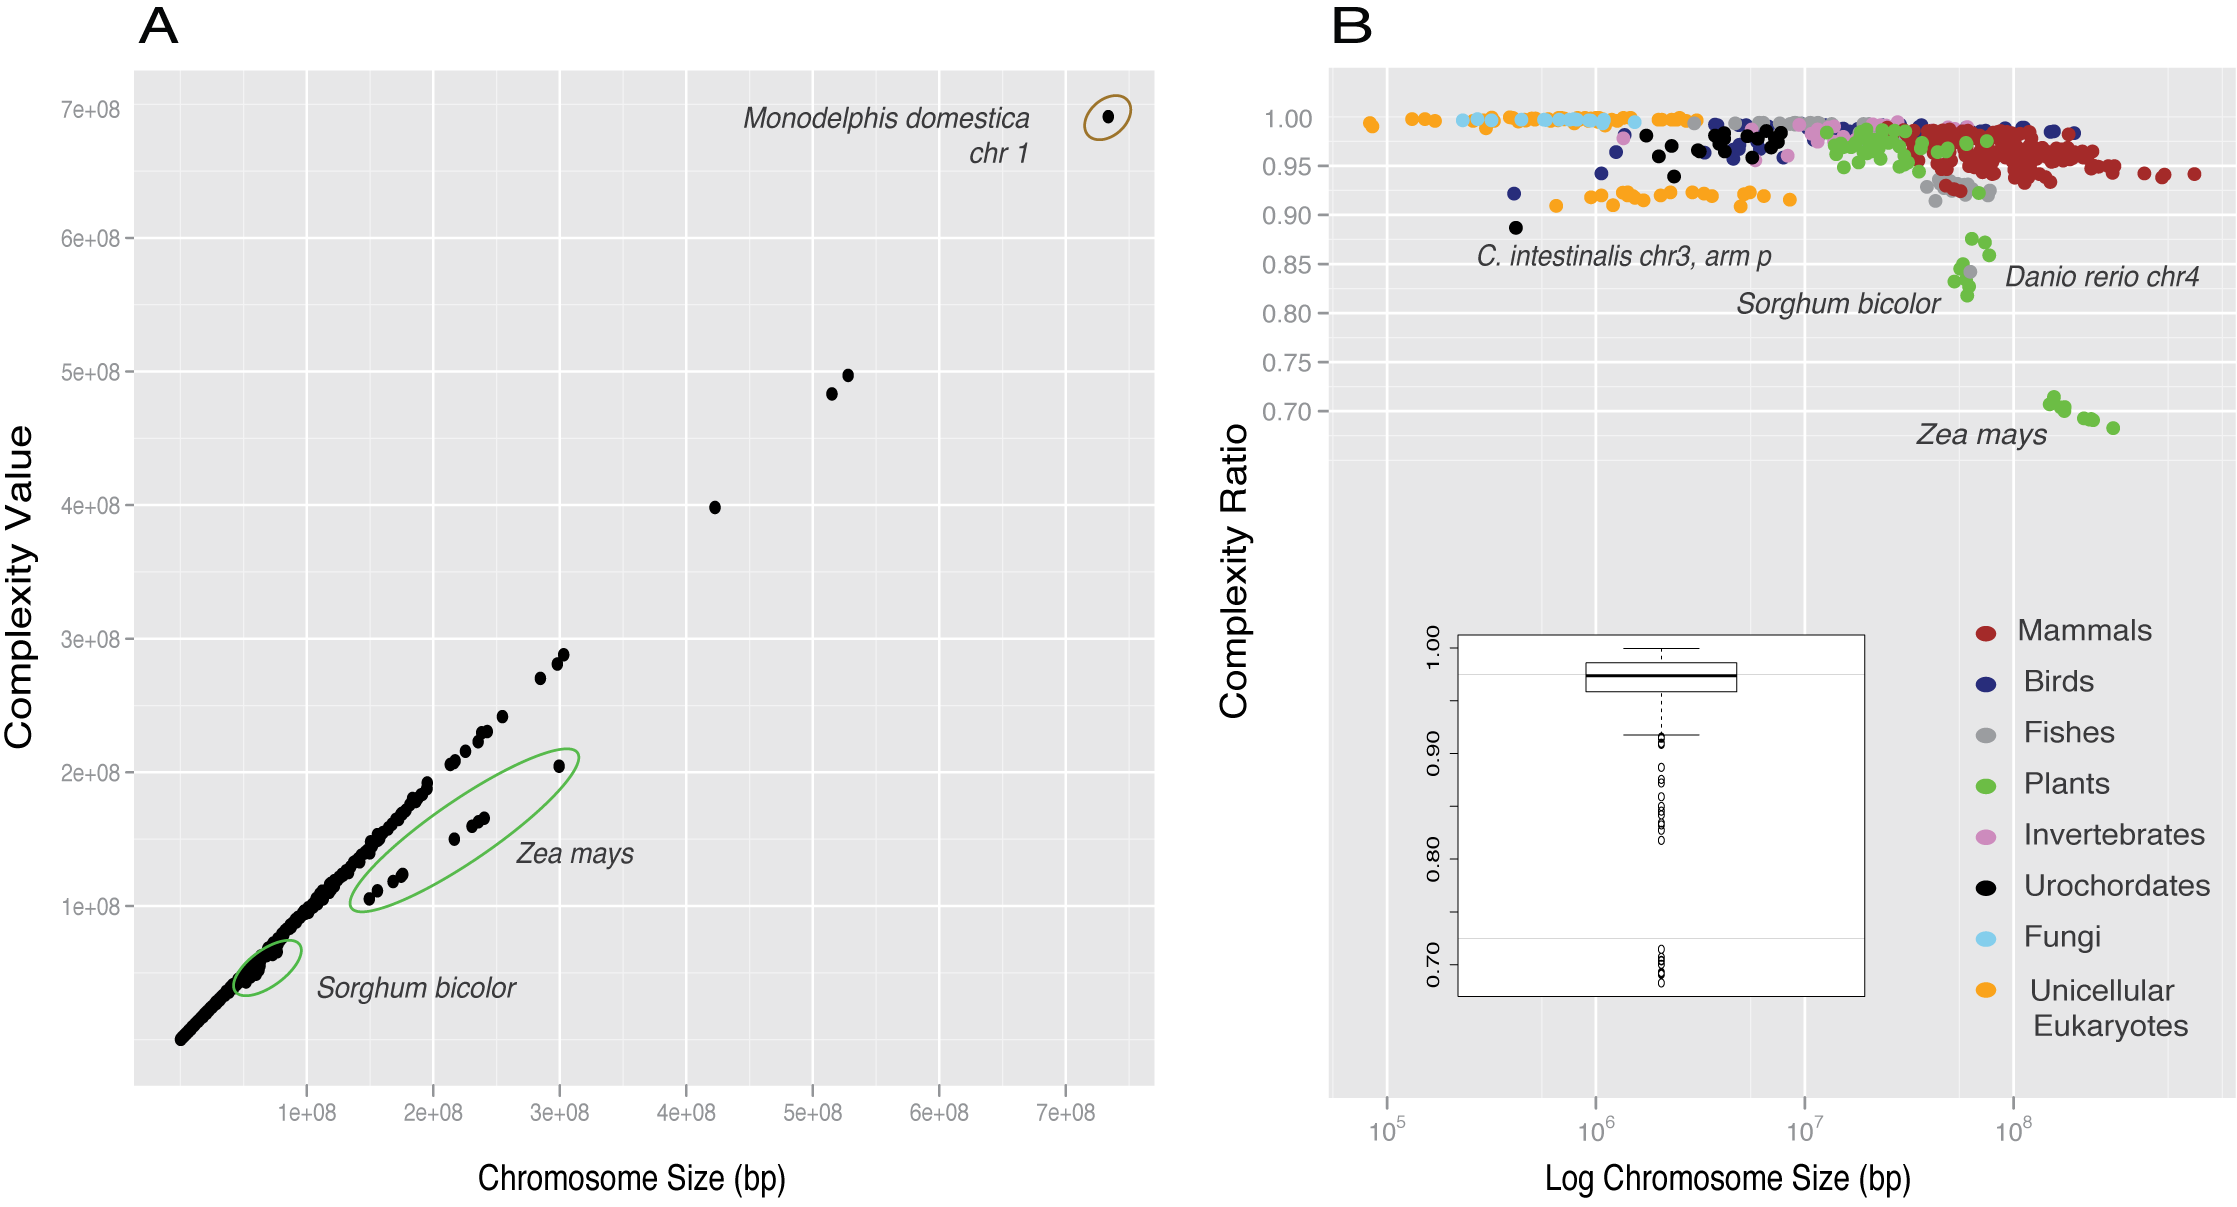
\includegraphics[width=\textwidth]{tex_source/figures/dna_struct/chromosome_complexity.png}
\caption[Chromosome complexity ratio]{{\bf Chromosome complexity ratio.} \\\textbf{(A)} Complexity ratio and chromosome size of 31 eukaryote species (567 chromosomes). Notice how far chromosomes of Z. mays, and in minor degree S. bicolor (both recent polyploid species) depart for the general trend. \textbf{(-B)} Most chromosomes (96.2\%) have complexity ratios ranging 0.9 to 1.0, as observed for complete genomes \fref{fig:gen_compl}{B}. Boxplot inside shows the distribution of CR of all
chromosomes.}
\label{fig:chr_compl}
\end{figure}

\subsection{Complexity in chromosome segments}
\label{sec:compl-chrom-segm}

Chromosomes were split in overlapping windows of various sizes (from 1 Kb to 100 Mb) and complexity ratio in these windows was computed. \fref{fig:box_compl}{} shows boxplots of six selected chromosomes, at different scales, all having extreme CR. Median values of CR over all windows of \textit{H. sapiens} Chr1 \fref{fig:box_compl}{-A}, \textit{A. thaliana} Chr1 \fref{fig:box_compl}{-C}, \textit{C. elegans} Chr1 \fref{fig:box_compl}{-D}, and \textit{D. melanogaster} Chr2L \fref{fig:box_compl}{-E} were above 0.97. Lower values were obtained in \textit{Z. mays} Chr 1 \fref{fig:box_compl}{-F} and in \textit{H sapiens} Chr19 \fref{fig:box_compl}{-B} for large windows sizes; in particular, for windows larger than 1Mb, CR noticeably fell down. The reasons for this fall are different in the two cases: while maize Chr1 is tetraploid, human Chr19 contains the highest number of Alu sequences reported in human chromosomes \cite{Venter2001}.

\begin{figure}[htpb] 
\centering 
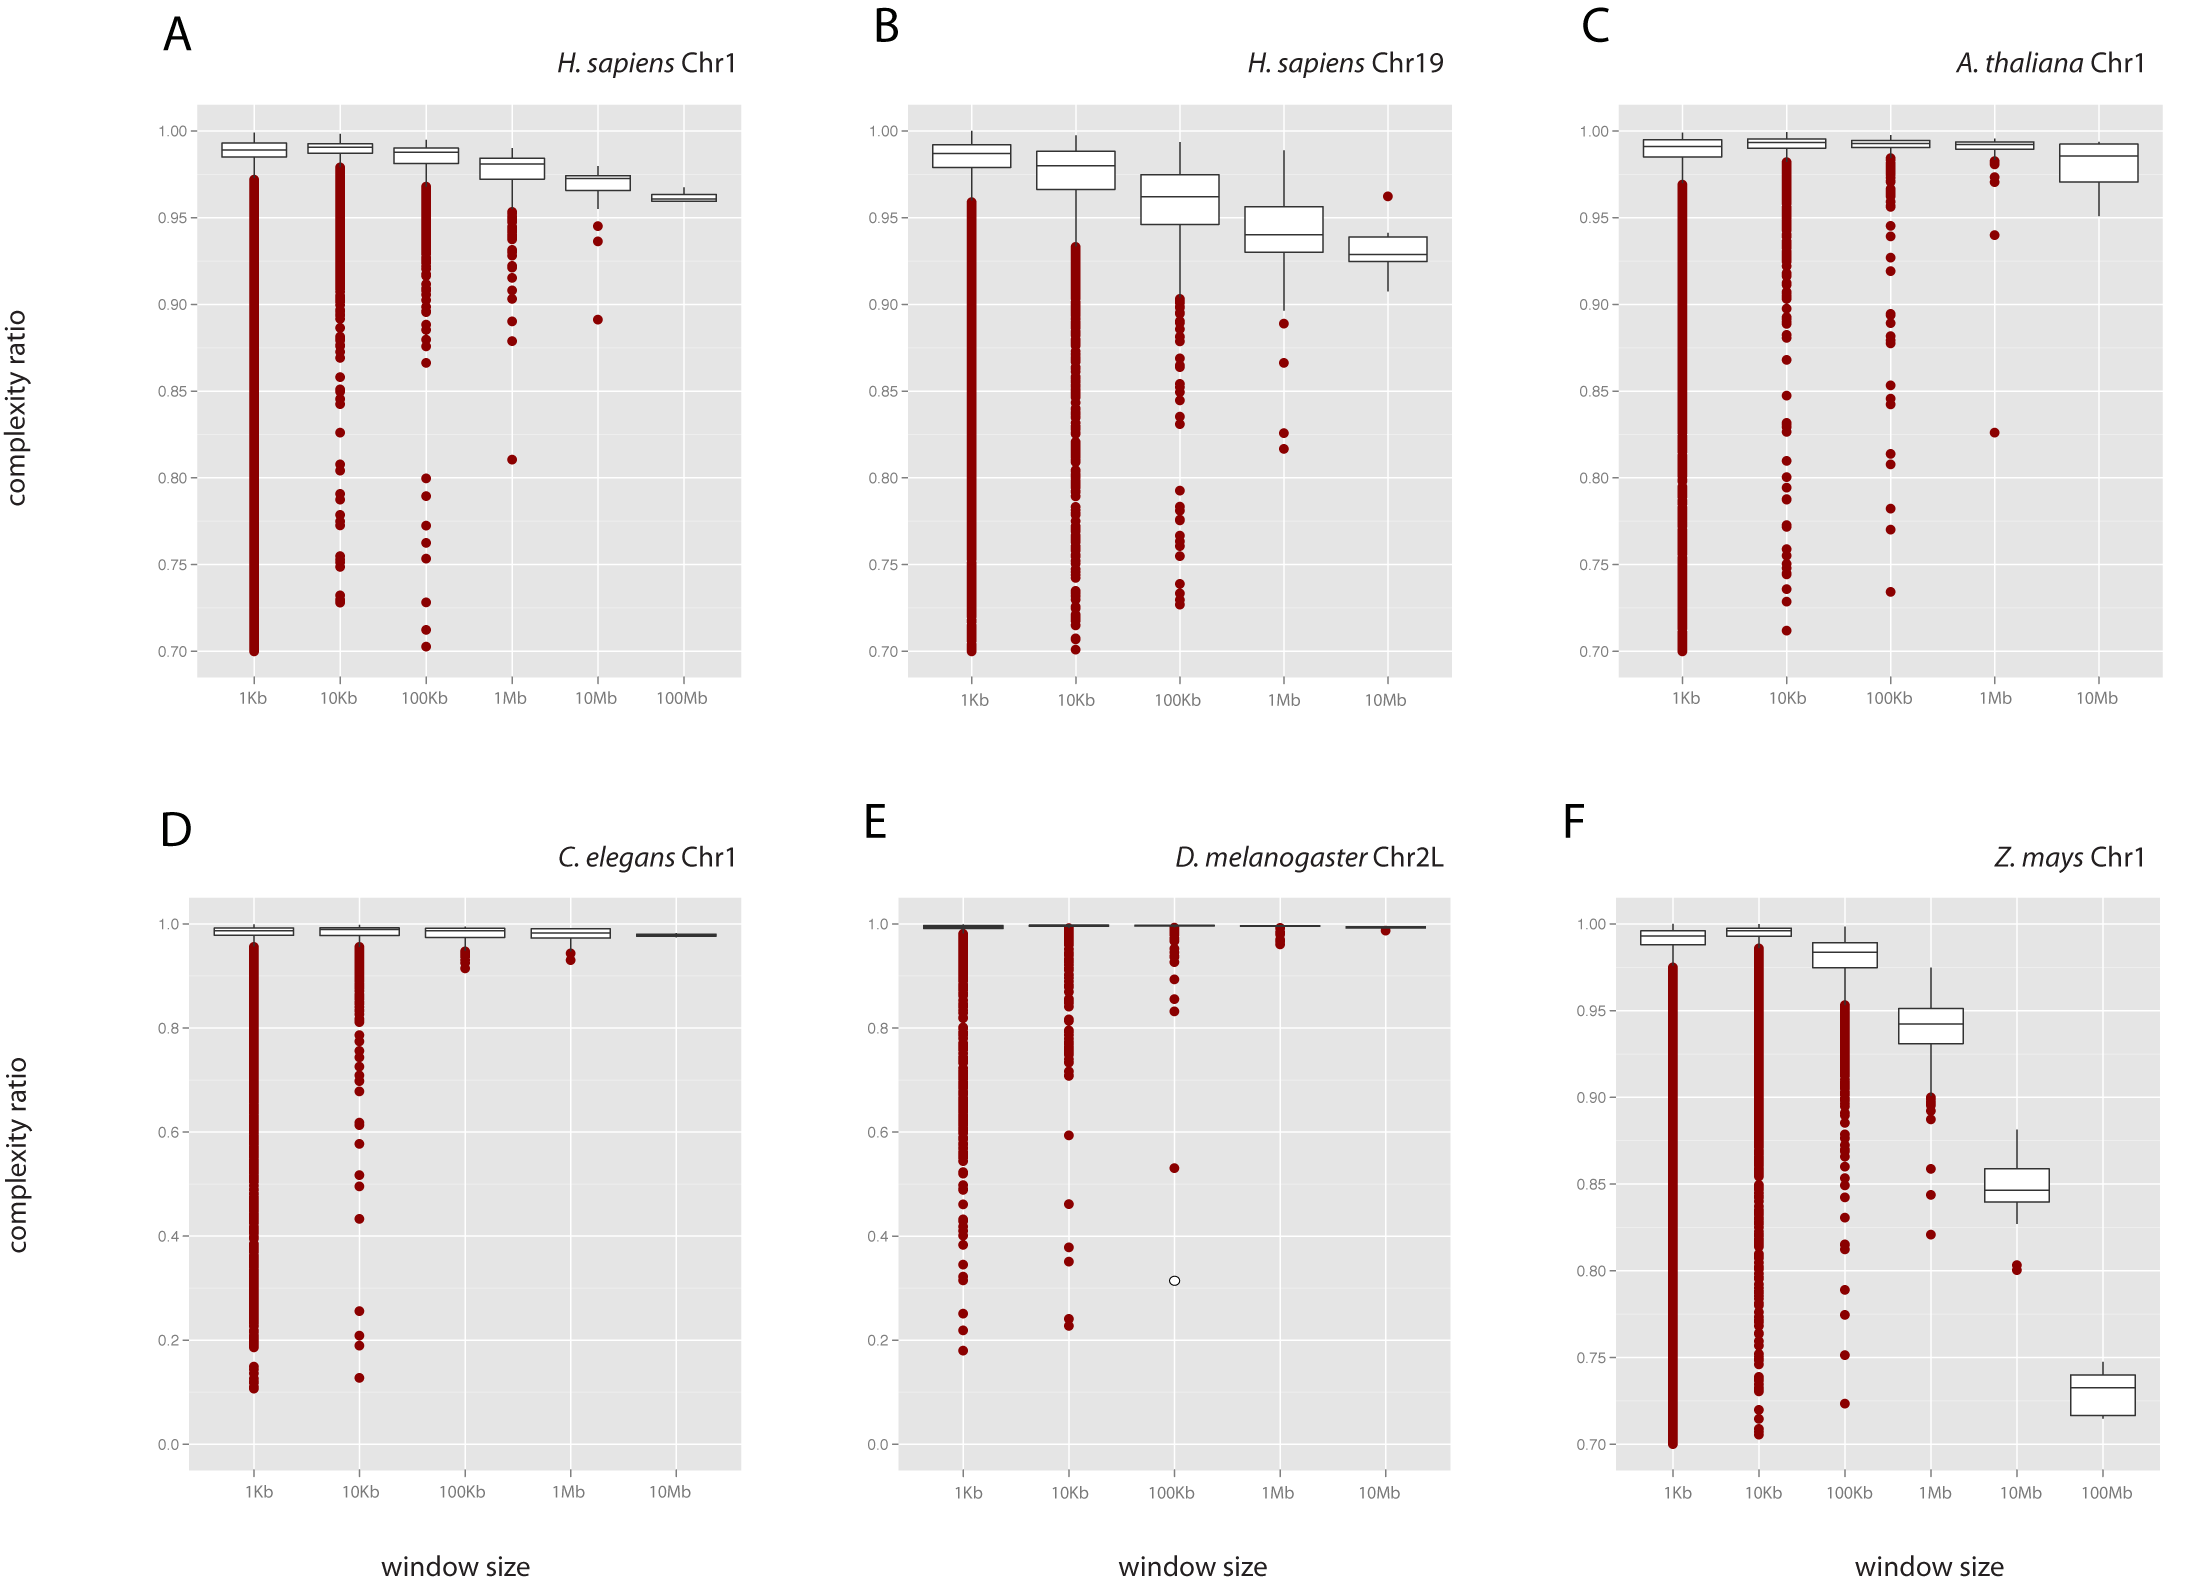
\includegraphics[width=\textwidth]{tex_source/figures/dna_struct/box_complexity_windows.png}
\caption[Sliding window analysis in chromosomes]{{\bf Sliding window analysis in chromosomes.} \\Boxplots show results of sliding window analyses in six selected chromosomes (A-F). Most chromosomes have median CR higher than 0.975 independently of window size. White dot in the 100Kb window size chart of D. melanogaster Chr 2L (E) corresponds to the ``deep spike'' displayed in \fref{fig:win_2L}{}. Scales were selected to enlarged differences in CR.
}
\label{fig:box_compl}
\end{figure}


In general, for all chromosomes, the larger the window size, the lower the median CR value. This pattern can be explained by existence of repeats, which can only be detected when the window size is large enough. In addition, CR dispersion decreases when window size increases, a fact that is explained by the substantial DNA combinatorial variation in large chromosome windows. This effect is shown in \fref{fig:win_2L}{} for window sizes of 1Kb and 100 Kb in \textit{D. melanogaster} Chr 2L, with a rugged versus smooth CR profiles. The outstanding
minimum CR ~ 0.31 was for 100 Kb-window size. This sudden decrement in CR occurred at 21,400 - 21,550 Mb where the histone cluster with more than 100 genes of the family locates.

\begin{figure}[htpb] 
\centering 
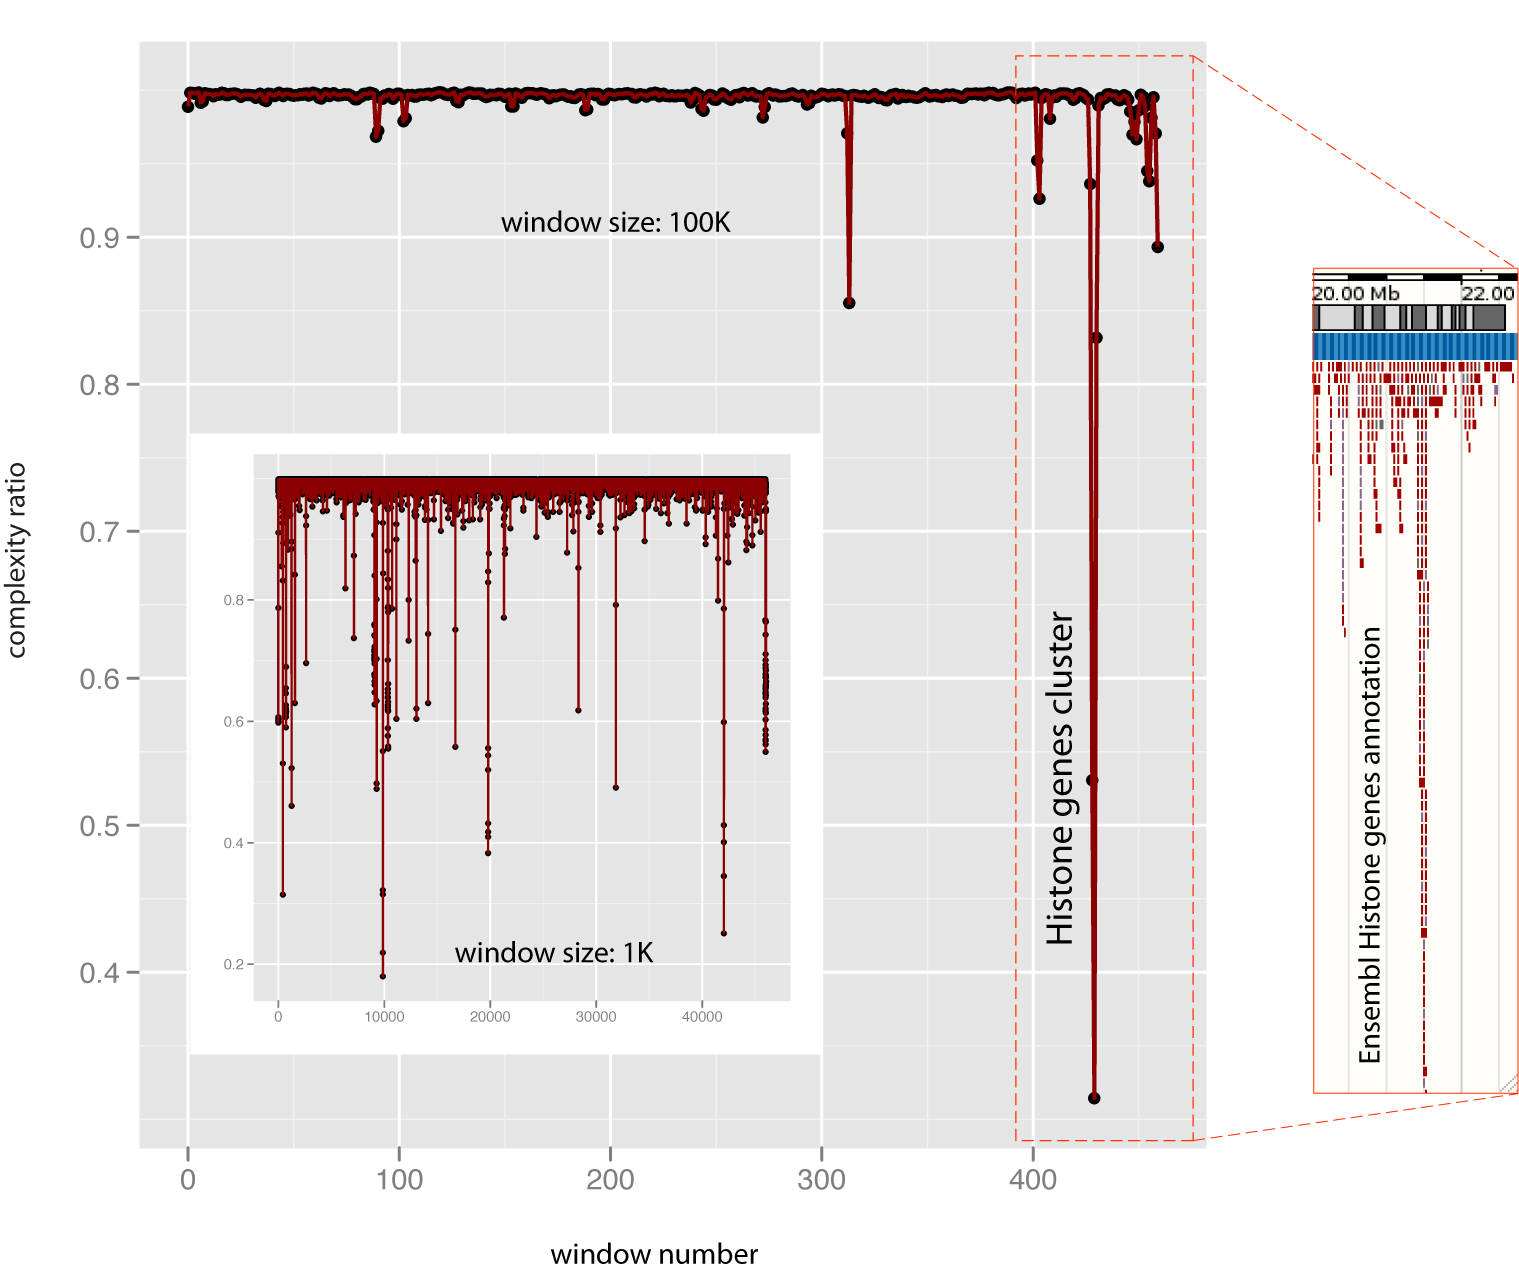
\includegraphics[width=\textwidth]{tex_source/figures/dna_struct/windows_2L.png}
\caption[Sliding window in a full chromosome]{{\bf Sliding window in a full chromosome.} \\Complexity ratio along \textit{D. melanogaster} chromosome 2L is displayed at two window size scales. Ensembl annotation of the histone genes cluster is shown in the left box. See associated DAS server displaying CR along chromosomes for 15 eukaryote species.
}
\label{fig:win_2L}
\end{figure}


The right picture shows Ensembl annotation for the histone genes cluster. The complexity values correspondind to an exhaustive sliding-window scan of chromosomes of fifteen different species is available in a DAS server at \myurl{http://bioinfo.cipf.es/das/} Complexity in repetitive elements and genes 

Eukaryote genome structure is generally sketched out by the massive presence of non-functional repetitive elements (RE-s) spread out all over the genome, and a tiny portion of singular functional elements covering the rest. To get insights into the statistical structure of these contrasting regions of genomes we computed the complexity ratio of genes and of each of the main families of RE's (as DNA-T, LTR, LINE, SINE and satellite). To do this, for each family, all units were concatenated in their original order in chromosomes, after scanning them with RepeatMasker  \cite{Smit2010} (see details of RepeatMasker output for individual species in Document S1).

Genes showed, as expected, the highest CR among all classes analyzed, independently of the species. When genes were split in their two main components, exons showed even a higher CR. Unexpectedly, high values of CR were also obtained in LINE, LTR and DNA-T (~\tref{tab:rep_compl}). In constrast, SINE and satellites showed the lowest CR. The low complexity ratio observed in SINE and satellites is mainly due to their repetitive structure, in the form of
orderly arranged short sized repetitions. The high CR associated to LINE, LTR and DNA-T (DNA-T) is explained by their larger length and their high internal variability in units of the families. In mammals DNA-T and LTR elements exhibited higher CR than LINE elements. This is not the case for fishes, some invertebrates and plants. In plants, LINE has the highest CR after genes (~\tref{tab:rep_compl} and see \fref{fig:lang_compl}{} for comparison among all eukaryote species analyzed).

\begin{table}[htbp]
\caption[Mean complexity ratio of some genome components]{Mean complexity ratio of some genome components in different species.}
\resizebox{410pt}{!}{%
  \begin{tabular}{ l r r r r r r r r }
  \hline
  \multicolumn{1}{l}{\textbf{Species}} & \multicolumn{1}{l}{\textbf{Satellite}} & \multicolumn{1}{l}{\textbf{SINE}} & \multicolumn{1}{l}{\textbf{LINE}} & \multicolumn{1}{l}{\textbf{LTR}} & \multicolumn{1}{l}{\textbf{DNA-T}} & \multicolumn{1}{l}{\textbf{Genes}} & \multicolumn{1}{l}{\textbf{Introns}} & \multicolumn{1}{l}{\textbf{Exons}} \\ \hline
  {\it H. sapiens} & 0.485 & 0.437 & 0.881 & 0.922 & 0.962 & 0.953 & 0.952 & 0.985 \\ 
  {\it P. troglodytes} & 0.491 & 0.442 & 0.885 & 0.926 & 0.962 & 0.967 & 0.965 & 0.993 \\ 
  {\it R. norvegicus} & 0.539 & 0.586 & 0.668 & 0.912 & 0.975 & 0.977 & 0.976 & 0.992 \\ 
  {\it M. musculus} & 0.595 & 0.576 & 0.74 & 0.875 & 0.973 & 0.973 & 0.97 & 0.991 \\ 
  {\it C. familiaris} & 0.6 & 0.487 & 0.911 & 0.974 & 0.982 & 0.982 & 0.98 & 0.993 \\ 
  {\it T. nigroviridis} & --- & 0.585 & 0.903 & --- & --- & 0.994 & 0.993 & 0.993 \\ 
  {\it D. rerio} & 0.628 & 0.43 & 0.796 & 0.791 & 0.824 & 0.942 & 0.936 & 0.988 \\ 
  {\it C. intestinalis} & 0.644 & 0.537 & 0.836 & 0.937 & 0.801 & 0.968 & 0.957 & 0.994 \\ 
  {\it C. elegans} & 0.52 & 0.401 & 0.93 & 0.94 & 0.827 & 0.978 & 0.957 & 0.99 \\ 
  {\it A. gambiae} & 0.232 & 0.438 & 0.805 & 0.902 & 0.771 & 0.992 & 0.992 & 0.9 \\ 
  {\it D. melanogaster} & 0.548 & --- & 0.81 & 0.744 & 0.81 & 0.985 & 0.982 & 0.99 \\ 
  {\it Z. mays} & 0.337 & 0.531 & 0.906 & 0.495 & 0.7223 & 0.962 & 0.956 & 0.975 \\ 
  {\it S. bicolor} & 0.345 & 0.619 & 0.966 & 0.602 & 0.757 & 0.99 & 0.991 & 0.988 \\ 
  {\it A. thaliana} & 0.467 & 0.675 & 0.971 & 0.84 & 0.896 & 0.989 & 0.986 & 0.988 \\ 
  {\it A. lyrata} & 0.417 & 0.457 & 0.928 & 0.772 & 0.826 & 0.994 & 0.988 & 0.996 \\ \hline
  \end{tabular}
}
\label{tab:rep_compl}
\end{table}


For each family, we used the complexity ratio to describe the disposition of the elements inside a chromosome. CR of linearly arranged elements was compared to the CR of shuffled elements. \tref{tab:compl_rep} shows these values for eight selected chromosomes of different species. CR in the linear arrangement was much lower in SINE and satellites than in the rest of the classes. This reveals a structure of identical or very similar repeats along neighbor chromosome segments. This pattern did not showed up in the other families. The notable exception was LTR of the maize chromosome, known to have expanded dramatically in recent evolutionary times \cite{Blanc2004}. All shuffled classes (including SINE and satellites) had a CR equal to one, or very close to one. This entails an almost uniform statistical distribution of DNA sequences in that class. This result point outs that genomes are plenty of genetic variation, even in regions where the expected pattern is the homogeneous repetition of almost indistinguishable units of RE's.

\rowcolors{1}{white}{white}
\begin{table}[htbp]
\caption[Complexity ratio of genome classes concatenated and shuffled]{Size and complexity ratio of different genome classes concatenated (CON), and shuffled (SHU) for selected chromosomes. Size in Mb.}
\resizebox{410pt}{!}{%
  \begin{tabular}{ l l r r r r r r r r }
  \hline
   &  & \multicolumn{ 2}{c}{\textbf{\em A. thaliana}} & \multicolumn{ 2}{c}{\textbf{\em C. elegans}} & \multicolumn{ 2}{c}{\textbf{\em H. sapiens}} & \multicolumn{ 2}{c}{\textbf{\em Z. mays}} \\ \hline
   &  & Chr 1 & Chr 5 & Chr 1 & Chr 2 & Chr 1 & Chr 21 & Chr 1 & Chr 10 \\ \hline
  \multicolumn{ 1}{c}{} & SIZE & 0.476 & 0.147 & 0.159 & 0.149 & 0.172 & 0.118 & 0.48 & 0.288 \\
  \multicolumn{ 1}{c}{Satellite} & CON & 0.223 & 0.299 & 0.489 & 0.547 & 0.519 & 0.567 & 0.325 & 0.309 \\ 
  \multicolumn{ 1}{l}{} & SHU & 0.889 & 0.968 & 0.962 & 0.975 & 0.972 & 0.987 & 0.961 & 0.948 \\ \hline
  \multicolumn{ 1}{c}{} & SIZE & 0.023 & 0.023 & 0.009 & 0.007 & 35.782 & 3.979 & 0.051 & 0.023 \\ 
  \multicolumn{ 1}{c}{SINE} & CON & 0.69 & 0.682 & 0.367 & 0.402 & 0.439 & 0.433 & 0.525 & 0.531 \\ 
  \multicolumn{ 1}{l}{} & SHU & 0.976 & 0.975 & 0.956 & 0.943 & 0.925 & 0.942 & 0.945 & 0.951 \\ \hline
  \multicolumn{ 1}{c}{} & SIZE & 0.121 & 0.146 & 0.039 & 0.026 & 26.321 & 3.778 & 1.454 & 0.739 \\ 
  \multicolumn{ 1}{c}{LINE} & CON & 0.975 & 0.972 & 0.93 & 0.982 & 0.874 & 0.905 & 0.899 & 0.916 \\ 
  \multicolumn{ 1}{l}{} & SHU & 1.000 & 1.000 & 0.999 & 1.000 & 0.999 & 1.000 & 1.000 & 1.000 \\ \hline
  \multicolumn{ 1}{c}{} & SIZE & 0.914 & 0.944 & 0.022 & 0.013 & 10.474 & 2.11 & 115.466 & 57.56 \\ 
  \multicolumn{ 1}{c}{LTR} & CON & 0.811 & 0.809 & 0.98 & 0.984 & 0.906 & 0.93 & 0.47 & 0.513 \\ 
  \multicolumn{ 1}{l}{} & SHU & 0.998 & 0.998 & 1.000 & 1.000 & 0.999 & 1.000 & 0.993 & 0.995 \\ \hline
  \multicolumn{ 1}{c}{} & SIZE & 0.68 & 0.541 & 0.704 & 0.518 & 3.734 & 0.552 & 6.066 & 3.109 \\ 
  \multicolumn{ 1}{c}{DNA-T} & CON & 0.883 & 0.887 & 0.81 & 0.84 & 0.95 & 0.98 & 0.7 & 0.74 \\ 
  \multicolumn{ 1}{l}{} & SHU & 0.999 & 0.999 & 1.000 & 1.000 & 1.000 & 1.000 & 1.000 & 1.000 \\ \hline
  \multicolumn{ 1}{c}{} & SIZE & 18.242 & 16.312 & 10.77 & 9.918 & 140.258 & 21.909 & 37.623 & 16.759 \\ 
  \multicolumn{ 1}{c}{GENES} & CON & 0.988 & 0.989 & 0.975 & 0.981 & 0.951 & 0.964 & 0.956 & 0.967 \\ 
  \multicolumn{ 1}{l}{} & SHU & 1.000 & 1.000 & 1.000 & 1.000 & 1.000 & 1.000 & 1.000 & 1.000 \\ \hline
  \multicolumn{ 1}{c}{} & SIZE & 5.318 & 4.73 & 6.074 & 4.94 & 130.429 & 20.696 & 22.229 & 9.735 \\ 
  \multicolumn{ 1}{l}{INTRON} & CON & 0.985 & 0.986 & 0.95 & 0.963 & 0.95 & 0.964 & 0.948 & 0.966 \\ 
  \multicolumn{ 1}{l}{} & SHU & 1.000 & 1.000 & 1.000 & 1.000 & 1.000 & 1.000 & 1.000 & 1.000 \\ \hline
  \multicolumn{ 1}{c}{} & SIZE & 12.925 & 11.582 & 4.694 & 4.979 & 9.829 & 1.213 & 15.394 & 7.024 \\ 
  \multicolumn{ 1}{c}{EXON} & CON & 0.988 & 0.989 & 0.991 & 0.991 & 0.983 & 0.99 & 0.972 & 0.976 \\ 
  \multicolumn{ 1}{l}{} & SHU & 1.000 & 1.000 & 1.000 & 1.000 & 1.000 & 1.000 & 1.000 & 1.000 \\ \hline
  \end{tabular}
}
\label{tab:compl_rep}
\end{table}


Polyploidy and return to maximum complexity Evolution erodes ancient footprints of genome polyploidy and diploidization (the process by which a polyploid genome turns into a diploid one) proceeds during time \cite{Wolfe2001}. As shown in previous sections, CR of recent polyploids is much lower than in non-polyploid, or in ancient polyploid species. Diploidization can be achieved by multiple mechanisms \cite{Wolfe2001}, being the gradual disintegration of the duplicated genetic material by random mutation. This is the simplest form. However, more dramatic mechanisms such as massive deletion, and transpositions of genetic material was reported in \textit{A. thaliana} \cite{Hu2011}. We tested the hypothesis that the complexity ratio of polyploid genomes increases along the diploidization process.

Polyploid origin and posterior decay of genetic redundancy was simulated by means of mutations and transpositions in random sequences of different lengths and ploidy levels, and in \textit{Z. mays} Chr1 and \textit{S. bicolor} Chr1 (Figure 5). In all cases, sequences under random mutation and transposition reached maximum CR=1 after a number of generations large enough. Larger sequences representing genomes or chromosomes increased their CR faster than shorter sequences. This is as expected in probability theory since each sigle choice (introduced by a random mutation or a transposition) in a large set is more informative than in a smaller set, because it makes a selection in a bigger space of possibilities. The dynamics of CR increase was identical for the maize and sorghum chromosomes and the simulated random sequences (Figure 5A). Figure 5B shows that genomes and chromosomes reached maximum CR=1 after many cycles of transpositions. Using a simulated genome with tetraploid structure, transposition preserved the relation that chromosome CR is higher than genome CR, along all generations up to convergence to maximum CR=1. This feature was reported above for maize and sorghum (see discussion on chromosome complexity ratio).

Once CR reached almost maximum complexity any signal of polyploidy is finally lost, and DNA structure is indistinguishable from diploid genomes. High complexity and random-like structure of DNA Excluding recent polyploids, high CR (almost maximum) was observed in complete genomes of organisms sampled in all diversity of life, in their chromosomes and along large enough chromosomes segments, and in shuffled arrangements of elements in individual genetic classes. We conjecture this is a universal feature of all genomic sequences. Polyploids were the only DNA sequences on which we obtained low complexity ratios, hence, they are the only DNA sequences with the distinguishing feature low CR: Low CR corresponds to a simple combinatorial structure of the sequence. 

The combinatorial structure of a sequence is a description of the observed arrangement of the symbols among all possible permutations of the same length. Sequences with many long repeats have low CR. Sequences with the minimum CR=0 consist of a single symbol (as $AAAAAAAAAA$) -this is the simplest combinatorial structure- so they are plainly compressible. Polyploid genomes of maize and sorghum have CR=0.585, and CR=0.786, respectively. Values that were close to the simulated tetraploid genomes (Fig 5B). It is also possible to achieve low CR in sequences without any long repeats, but with an orderly arrangement of the symbols. Although we have not found this phenomena in natural DNA, we constructed de Bruijn sequences (these are the mathematically defined sequences with perfect equifrequency of subsequences: every possible sequence of logarithmic length appears exactly once as a sequence of consecutive symbols) \cite{DeBruijn1946,Becher2011} with low CR. The regularity in the combinatorial structure of these particular de Bruijn sequences is captured by the MTF algorithm. See Appendix I for examples on short sequences. High complexity ratio implies the following properties on the combinatorial structure of DNA sequences: High CR corresponds to high diversity and balanced abundance of short repeats. Maximum CR=1 is reached by sequences a sequence of length n if it contains full diversity of length k, for k ! log4 n, and each these short sequences occur about n*4-k times. As CR decreases, diversity and balanced abundance deteriorates. In particular, maximum CR is holds for some de Bruijn sequences \cite{DeBruijn1946,Becher2011}. Also maximum CR=1 occurs in randomly generated sequences with uniform distribution of A, C, G, T. For genomic sequences \cite{Liu2008} reported that more than 98\% of 12 bp oligomers appear in vertebrate genomes while less than 2\% of 19 bp oligomers are present. For the human genome we computed all maximal exact repeats over 30 bp, and counted their diversity and quantity \cite{Nies2009}. We observed that the largest correlations in the human genome are intrachromosomal, the actual largest exact repeat is 67,632bp long and it occurs just twice inside Chr 1, while the largest inter-chromosomal perfect correlation is 21,865 bp occurring just once Chr 1 and once in Chr 5.

High CR corresponds to random-like sequences. Intuitively, a non random sequence will exhibit some significant regularity that can be used to compress the sequence. The mathematical underpinning relies on the theory of pure randomness \cite{Chaitin1975,Nies2009}, which states that an infinite sequence is random when its initial segments are incompressible. Up to some deviations, for finite sequences and particular compression methods, the identification between statistical randomness and incompressibility holds. The complexity ratio (CR) expresses incompressibility by the BWT-MTF scheme and further encoding as determined by Shannon's entropy. High complexity ratios correspond to highly incompressible sequences, which are sequences with a random-like structure. As in statistical randomness, the number of sequences with high CR grows exponentially with the sequence length. Thus, each genome is a singular instance out of the extraordinary many combinatorial variants of the same length with the same high complexity rate. A lower bound of the number of sequences with high CR (CR `` 1 - !, for any real value ! between 0 and 1) is proved Appendix II.


\section{Material and methods}
\label{sec:dna_struct-matmet}

\subsection{The complexity ratio and complexity value}
\label{sec:compl-ratio-compl}

Complexity Ratio (CR) is defined by a classical formula used in data compression \cite{Adjeroh2008}, the Burros-Wheeler transform BWT \cite{Burrows1994}, followed by the Move To Front (MTF) \cite{Ryabko1980} and finally resume this to one value using Shannon's entropy \cite{Shannon1948}. Thus the CR is Shannon's entropy of a transformation or digestion of the sequence. The purpose of this transformation is to reveal the regularities in a sequence. In case the original sequence has no significant regularities, all numbers will be at the same rate; else, some numbers will be in excess and others in shortage (compression algorithms use this to obtain a short output). Shannon's entropy is zero -this is the minimum- only when all numbers are zero. This occurs when a sequence consists just of a single repeated symbol, which is the simplest possible combinatorial structure. When, at the other edge, entropy is equal to one (the maximum entropy), then all numbers have exactly the same frequency, and it indicates that the sequence has a random-like combinatorial structure. 
Algorithmically, the BWT of a given sequence is a permutation of the symbols in the sequence that represents the lexicographic order of all possible rotations of the sequence. The MTF transforms a given sequence into a sequence of numbers, operating from left to right, and maintaining a stack of recently used symbols. Each number is an index in the stack and denotes an alphabet symbol. Shannon's entropy maps a sequence into a real number between zero and one. It weights the frequency of the alphabet symbols in a given sequence. For each symbol $i$ in the alphabet, let $p_{(i)}$ be the probability of finding $i$ in the sequence $s$; $N_i$ the number occurrences of $i$ in $s$ and $length(s)$ the total length of the sequence $s$: 

\begin{equation} \label{eq:prob_seq}
p_{(i)} = \frac {N_i}{length(s)}
\end{equation}

For DNA alphabet entropy is defined as:

\begin{equation} \label{eq:entropy}
E(s) = -\sum_{i=0}^{\exists}p_{(i)} \times log_4(p_{(i)})
\end{equation}

Thus the CR can be factorize as:

\begin{equation} \label{eq:cr}
CR(s) = E(MTF(BWT(s)))
\end{equation}

The complexity value (CV) of a sequence is its CR times the number of
characters in this sequence (here $s$):

\begin{equation} \label{eq:cv}
CV(s) = E(MTF(BWT(s))) \times length(s)
\end{equation}

As the CV of a sequence depends on the transformation of the MTF applied to the whole sequence, its computation impede the use of parts of the sequence independently.

\subsection{Complexity in strings}
\label{sec:complexity-strings}

Complete genomes of 54 species were download from NCBI and Ensembl Genome Project \cite{Flicek2011}. Fourteen major groups of taxa were selected: virus, phages, bacteria, archaea, fungi, amplicomplexa, heterokonta, amebozoa, urochordates, invertebrates, plants, fishes, birds, and mammals. Species among taxa were chosen to the interest as model species and the presence of particular biological features such as: variation in genome size, ancestral and recent polyploidy, living in extreme environments, living as intracellular parasites, gene expansion, genome reduction, RNA or single-strand DNA genomes, and synthetic genomes \tref{tab:genome}. Eukaryote genomes with coverage of 6$\times$ or greater were chosen. Sexual chromosomes were excluded from the analysis, and ambiguous ``N'' characters were removed from sequences, and not taken into account when computing chromosome length. Eukaryote chromosomes were concatenated in genomes to estimate genome complexity. Interspersed repeats and low complexity DNA sequences were screened and mapped in chromosomes of thirty different eukaryotes using RepeatMasker \cite{Smit2010}. Complexity of major families of repetitive elements such as DNA transposons, LTR, LINE, SINE, satellites and exons, introns, and complete genes (considering unstranslated regions) was computed after concatenation of all elements in chromosomes excluding. Random sequences with different ploidy levels were generated in python. Complexity value of biological sequences and random sequences was computed with the DNA alphabet of four letters. Complexity in biological sequences was computed in the +1 strand. Analyses of -1 strand provided no differences in results. Short stories, books and complete works in its original languages were downloaded from Project Gutember (\myurl{http://www.gutenberg.org/}). To automatically detect the alphabet size in texts (including mathematical and punctuation symbols) we run COMPL program with ``auto'' option. To study complexity along chromosomes, a sliding window method shifting along chromosomes in overlapping units of 1.0 Kb to 100 Mb was performed. Linear models, and linear models with interactions were run in R language \cite{Team2008}.

\subsection{Simulations}

We performed four kinds of experiments where complexity value and ratio were computed. First: random polyploid construction of sequences of various sizes and ploidy levels (one to ten). Second: the evolution along 40 million generations by constant neutral mutation rate of 1.0e-08 mutations per site per generation (this value is in between the mutation rate estimated for {\it Homo sapiens}: 2.5e-08 \cite{Nachman2000} , and \textit{Arabidopsis thaliana}: 7.1e-09 \cite{Ossowski2010}) on random sequence, and on chromosomes of \textit{Zea mays} and \textit{Sorghum bicolor}. Third: the evolution along 50,000 generations of random polyploid genomes of different sizes (100Kb, 1Mb, 10Mb) by transpositions of a fixed length (1.0 Kb) between chromosomes. The number of transposition per generation was set as a constant function of genome size (genome size/1,000). Last: the concatenation and shuffling (computed with the python base function: ``shuffle'') of all repetition instances in chromosomes for main repetitive families, and genes were considered. Complexity value and ratio were computed every 100 generations. 

\section{Discussion}

However it is striking that whatever subgroup of elements we selected (\textit{Simple repeats}, \textit{Satellites}...), no perfect random structure was found in any of the steps of life complexity. Sequences can be divided into modules of nucleotides as mentioned in \cite{Wagner2007} or defined by Herzel and collaborators \cite{Herzel1995} when it fulfill 3 requirements, concisely:
\begin{itemize}
\item \textbf{Requirement 1}: must occur more frequently than expectation by random.
\item \textbf{Requirement 2}: must not be included into a larger module.
\item \textbf{Requirement 3}: must be non-overlapping between them.
\end{itemize}

%%% Local Variables: 
%%% mode: latex
%%% TeX-master: "../../master"
%%% End: 


\chapter{Life inside genomes, dynamics and predictions}
\label{chap:untb_genomes}
%%% untb_genomes.tex --- 

\section{Background}

Whatever the environment, terrestrial or aquatic, temperate or tropical it is universal the case that some species are very abundant, others are relatively common, and the majority, rare. What mechanisms control this uneven distribution of species abundance in ecological communities?

Species diversity and their relative abundance have always intriguing ecologists \cite{McGill2007}. Roughly speaking, ecological models of species abundance are of two kinds: descriptive (statistical-based) or mechanistic (niche-based or neutrals). While many mechanistic approaches assume niche differences as the main cause driving community composition, neutral models consider niche differences among species irrelevant \cite{Margurran2004}. The unified neutral theory of biodiversity (UNTB) \cite{Hubbell2001,Rosindell2011} is a neutral-stochastic theory originally inspired in neutral population genetic models \cite{Kimura1985,Wright1931}. UNTB assumes interactions among trophically similar species equivalent on an individual ''per capita'' basis. This provocative assumption means that these individuals, regardless of the species, appear to be controlled by similar birth, death, dispersal, and speciation rates. Since each species follows a random walk, biodiversity composition emerges regardless of specific species differences in the community. The fundamental biodiversity parameter ($\theta$), analogous to $4N\mu$­ of population genetics, governs species richness in spatial and temporal scale. Neutral theory is thus a useful null model against to test alternative biological hypotheses of relative species abundance distribution \cite{Volkov2003,Alonso2006}.

Likewise ecological communities, eukaryotes genomes contain a variable number of more or less abundant elements of different genetic classes: transposon-derived elements, satellite repetitive sequences, segmental duplications, and their less abundant functional sequences such as RNA or genes. Here, for simplicity we talk of genetic elements of different classes as individuals of different species.

Dynamical ecological models of genomes were formalized and simulated \cite{Abrusan2006,Leonardo2002,LeRouzic2007}. Some complex models parallel interactions like parasitism, competition and cooperation between different families of transposable elements (TEs). However, ideal models of genomics would consider not only TEs, but also all diversity of genetic elements populating eukaryote genomes: satellites sequences, DNA-transposons, LTR-retrotransposons, LINES, SINES, mi-RNA, rRNA, tRNA, genes, and pseudogenes among the many functional and non-functional elements. Such model does not exist for genomes.

Here, taking advantage of the methods and models developed by ecologists we ask: is there a common pattern behind the relative abundance and diversity of genetic elements in genomes? And, in the case that such pattern exists, is it sufficient to explain together diversities of  functional and non-functional components in eukaryote genomes? To what extent abundance and diversity of genome components reflects adaptive or stochastic outcomes? Here we test the statistical adjustment of the UNTB predictions to more than 30 different eukaryote genomes.

To achieve this objective we discuss results in three different sections. First we analyze genomes and chromosomes by virtue of relative species abundance (RSA) curves, classical graphical tools used in ecology to know if genomes and chromosomes display uneven species distributions as is universally observed in ecological communities. Second we simulate the random distribution of all elements of genomes in all their chromosomes to statistically test the role of chance in chromosome design. Third, we test the statistical adjustment of the neutral ecological theory of biodiversity to the relative abundance and diversity of functional and non-functional elements of eukaryote chromosomes.

We conclude that abundances and diversity of genetic elements in most chromosomes is predicted by the stochastic dynamics of a model for which the principle of functional equivalence among elements is the primary assumption. Finally, we present a strong test to the hypothesis. If functional and non-functional genetic elements are distributed stochastically in chromosomes, their length must be predicted by demographic parameters only. Ecologists assert that effects of natural selection are dispensable to model abundance and species diversity in tropical forest \cite{Jabot2011}. Paralleling ecological communities Darwinian dynamics seems to be irrelevant to define abundance and diversity of genome components.

\section{Results}

\subsection{Genomic elements, dispersion and abundance}

Ecologists frequently use RSA curves to compare the richness, the degree of dominance, and the number of rare species in communities. The raw data used in these plots is the total number of individuals per species sampled in the ecosystem. The most interesting property of RSA curves is that species are unlabeled in the ranking order; hence ecosystems can be compared whatever the species they contain.

Taking advantage of the current automatic methods of genome annotation and string recognition, all genetic elements belonging to different functional and non-functional classes were counted to build RSA curves in genomes and chromosomes. These numbers represent censuses of genomic elements analogous to those sampled in ecosystems.

\begin{FPfigure}
\centering 
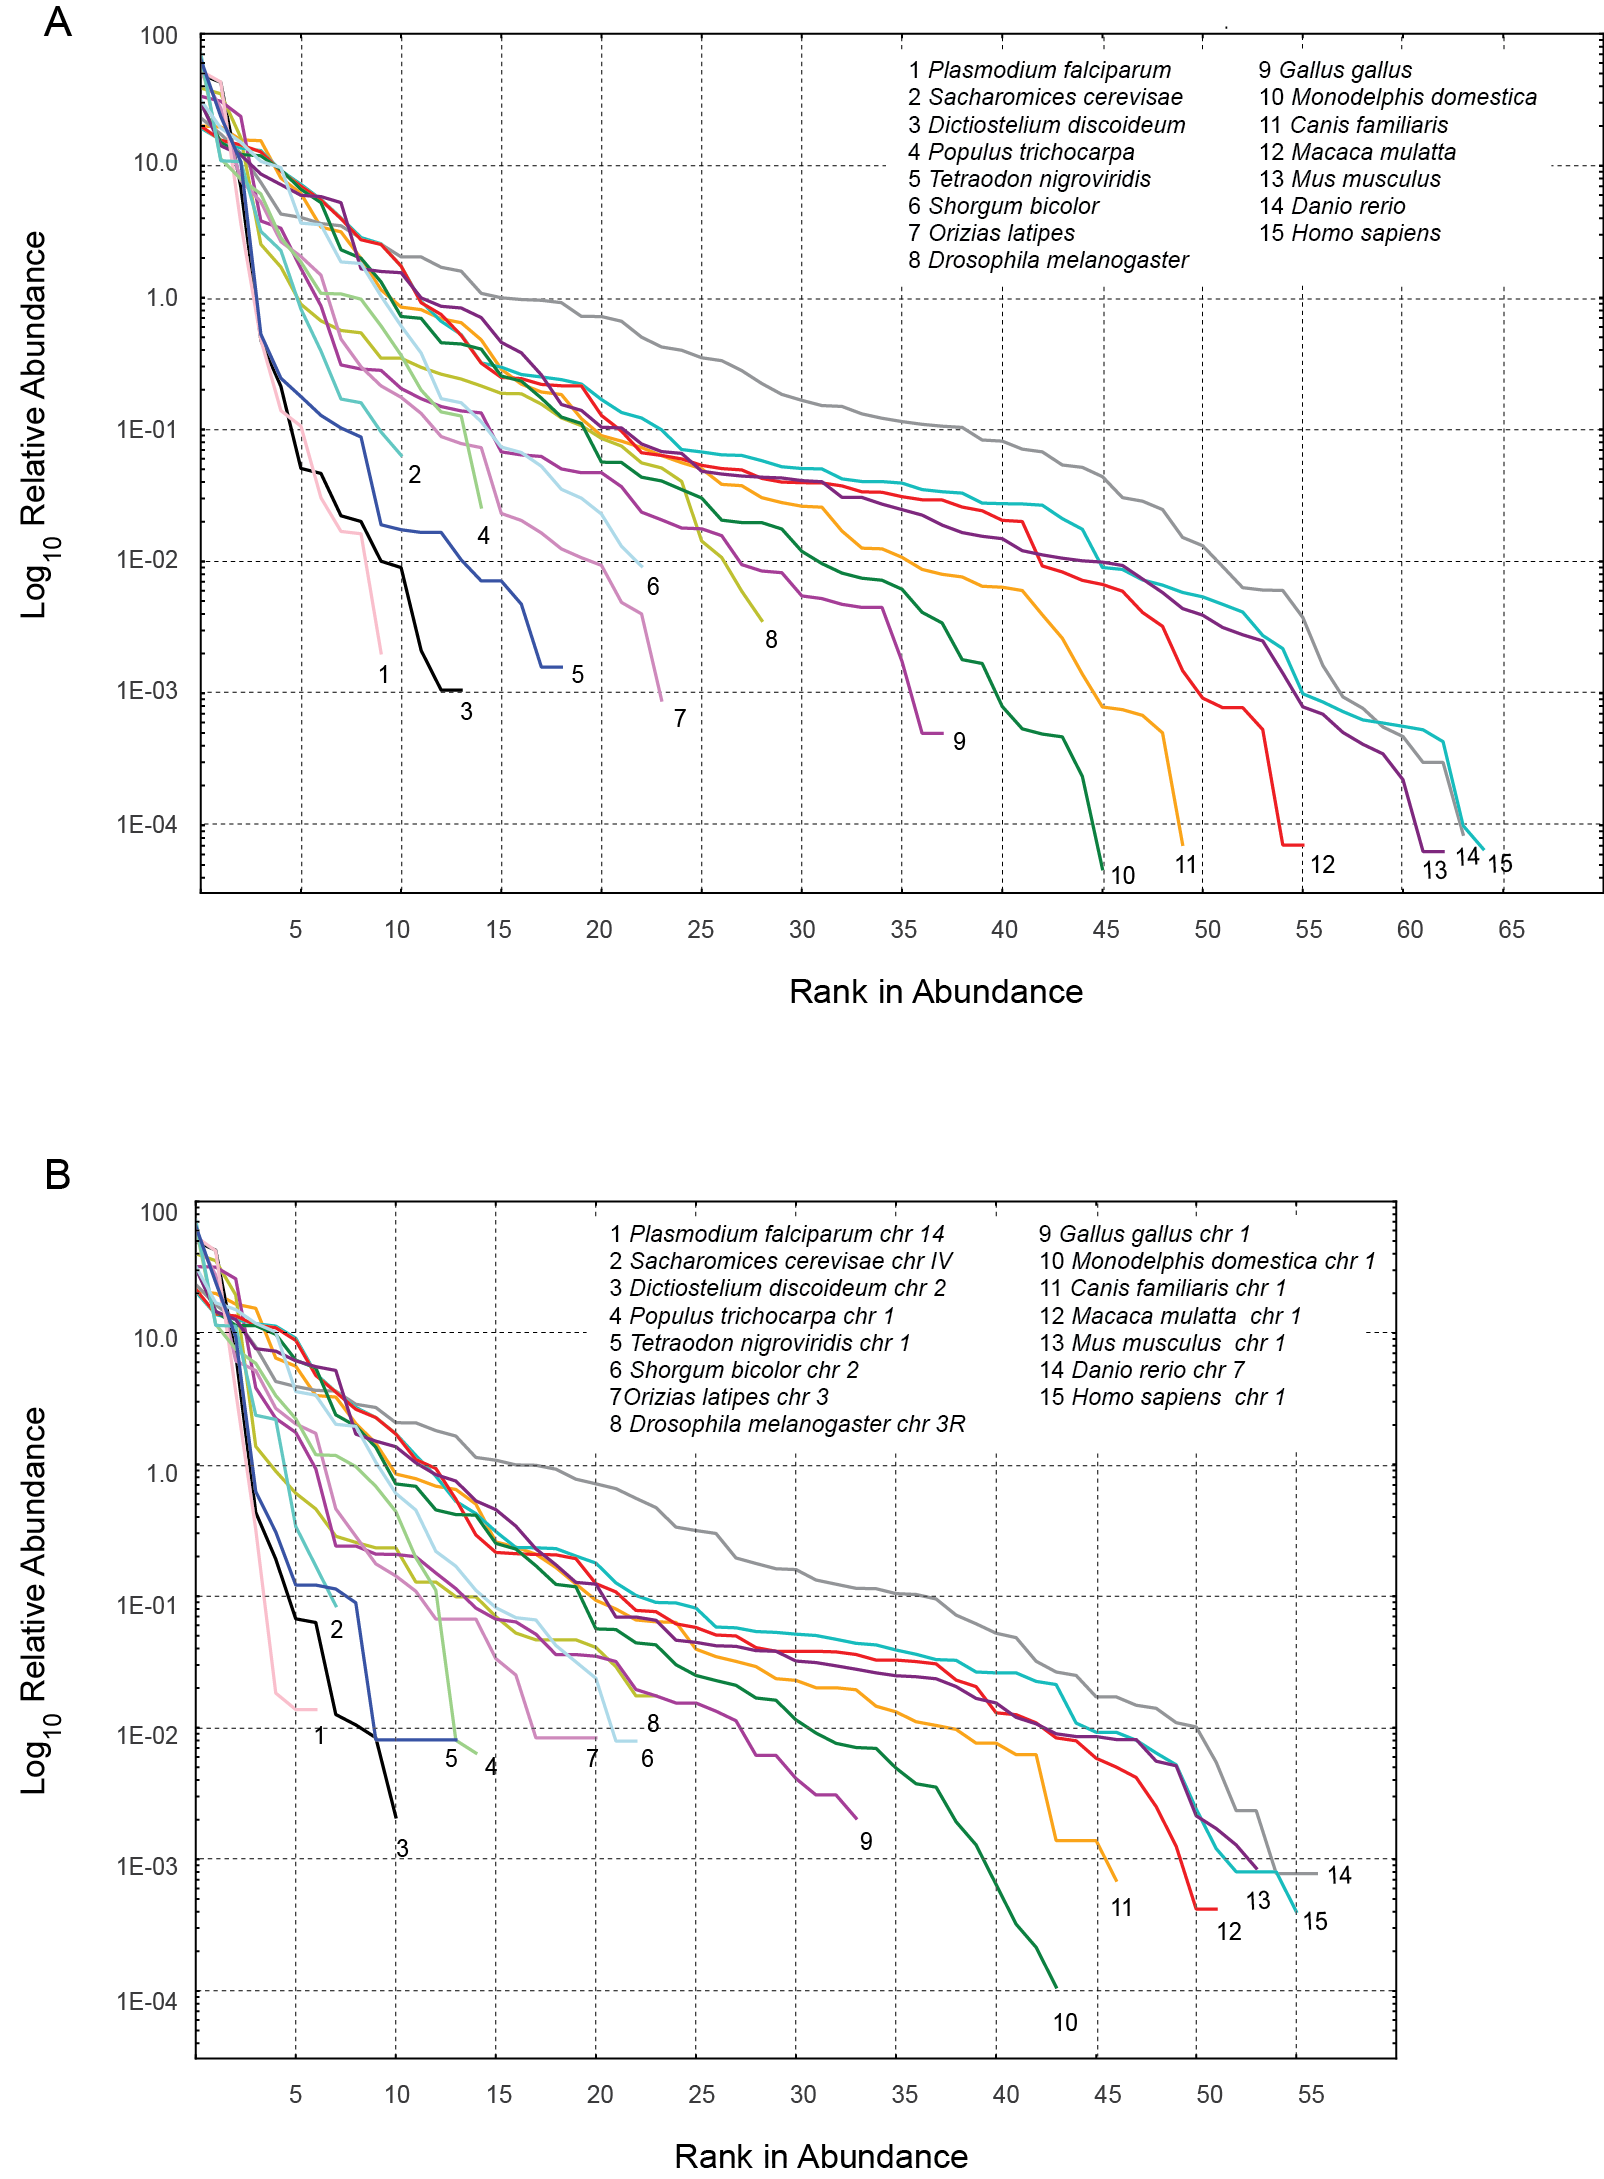
\includegraphics[width=\textwidth]{tex_source/figures/untb_genomes/SAD_genomes.png}
\caption[RSA curves.]{{\bf RSA curves.} \\ Relative species abundances for some selected genomes (A) and their corresponding largest chromosomes (B)} 
\label{fig:rsa_genomes}
\end{FPfigure}

\fref{fig:rsa_genomes}{} display RSA curves for a selected group of genomes and their largest chromosome respectively. Curves differ in many ways although two patterns are evident: 1- RSA curves of genomes and chromosomes are very similar for species, 2- all RSA curves display the universal S-shape observed in ecological environments \cite{McGill2007,Hubbell2001}. Both observations suggest a common mechanism of distribution of genetic elements in genomes and chromosomes.

\subsection{Counterbalanced species abundances in genomes}

To what extent chromosome's RSA curves represent the random distribution of the complete set of elements of the genome? To answer, we simulate the random distribution of the full set of genetic elements reported in genomes in their corresponding chromosomes. After one thousand simulations the mean expected abundance and its standard deviation were computed for all genetic classes in chromosomes. These values were used to plot random expected RSA curves for chromosomes.

Statistical tests (t-test, $FDR<0.05$) established that less than 1\% of all genetic classes in all chromosomes tested showed abundances according to their random expected distribution. This homogeneous process therefore, does not account for the observed RSA curves in chromosomes. However, another kind of arbitrary process is suggested for chromosomes if simulated and observed RSA curves are superimposed \fref{fig:rsa_chromosomes}{}.

\begin{FPfigure}
\centering 
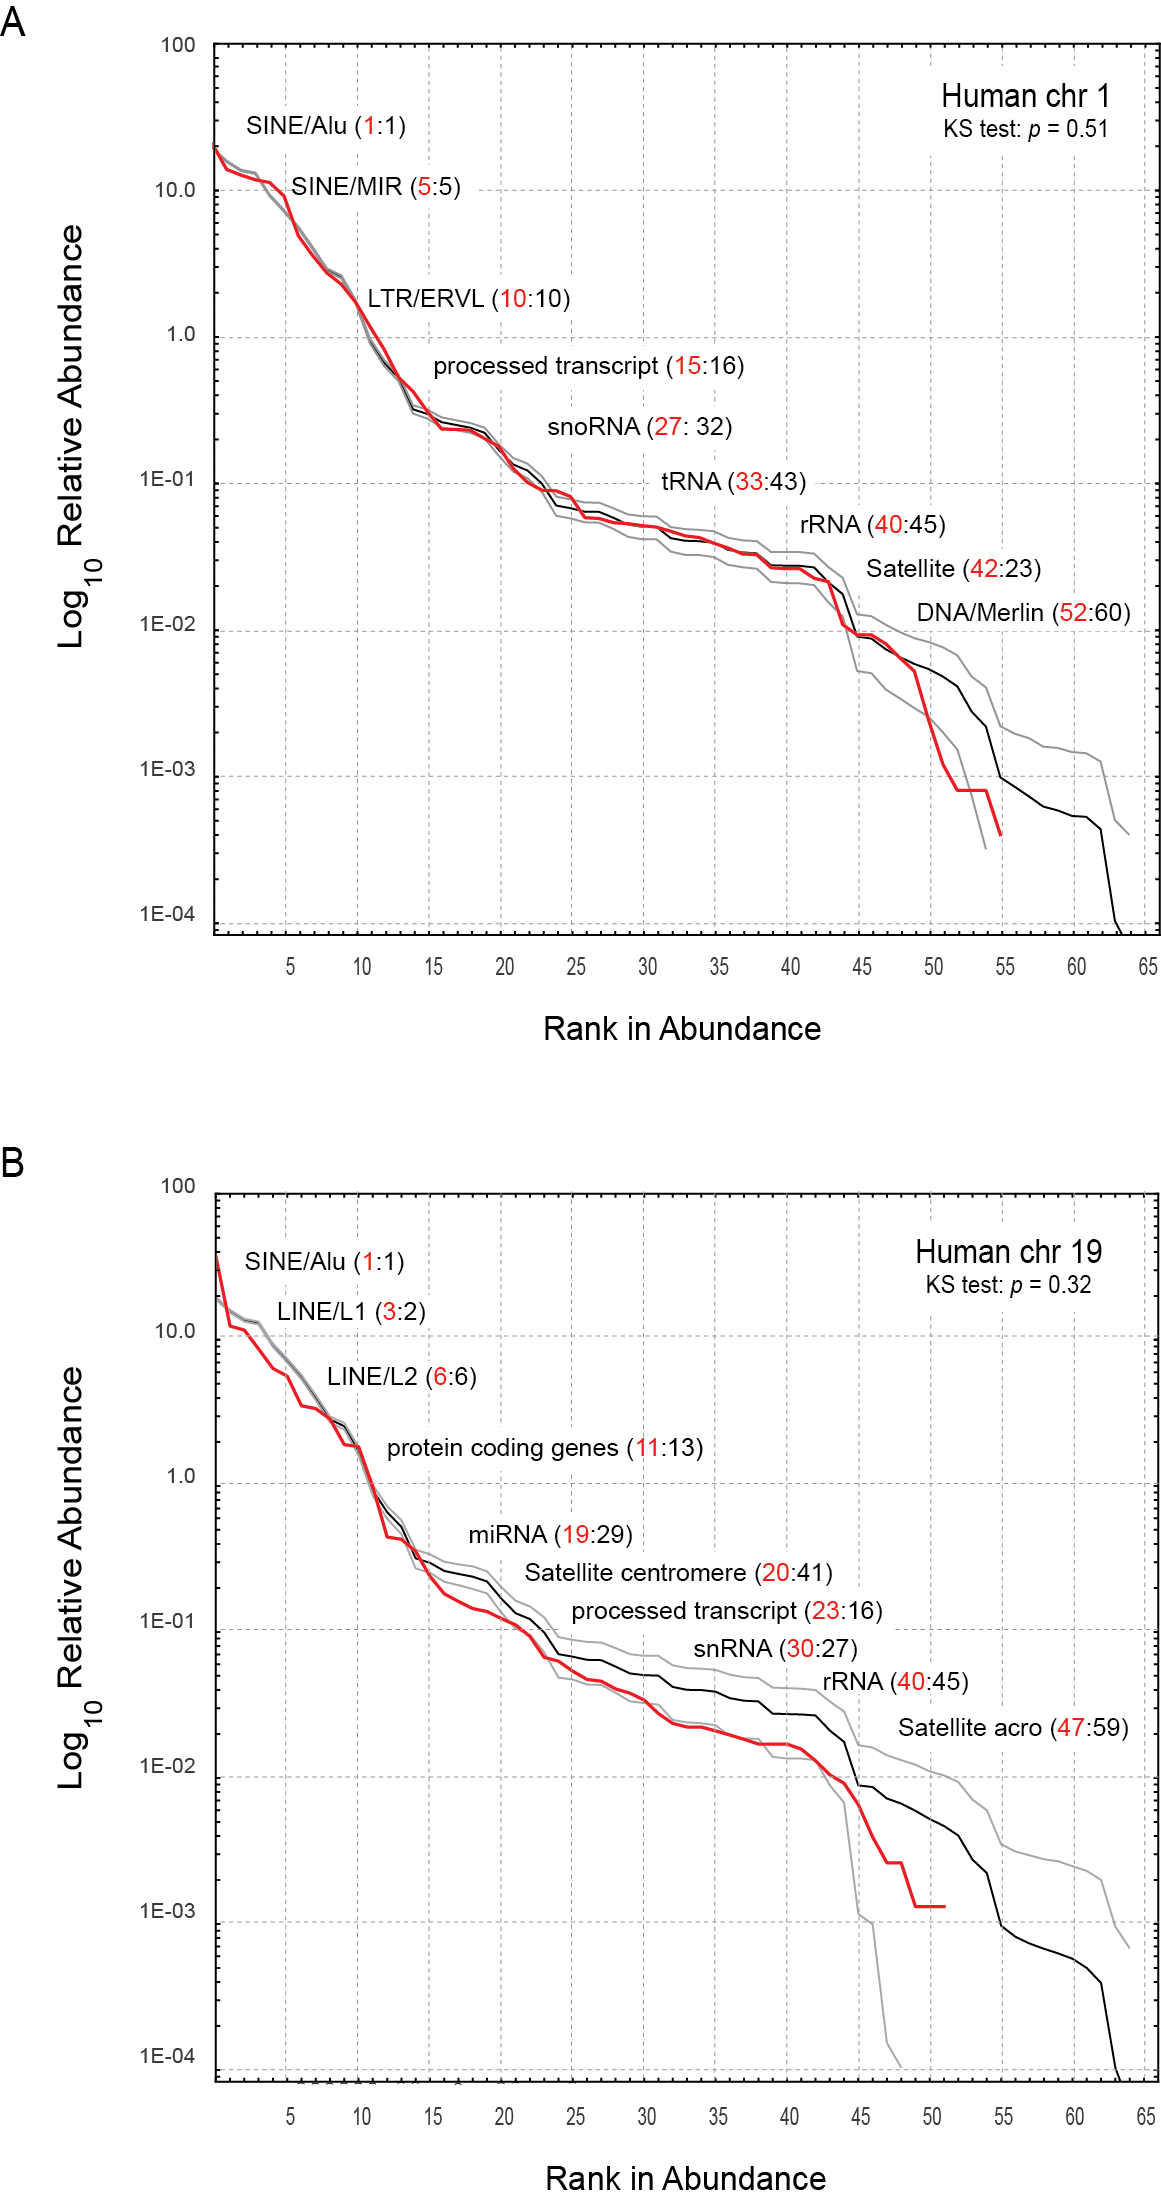
\includegraphics[height=\textheight]{tex_source/figures/untb_genomes/ra_chroms.png}
\caption[Relative species abundance curves for human chr 1 and chr 19]{{\bf Relative species abundance curves for human chr 1 (A) and chr 19 (B).} \\ Relative species abundance curves for human chr 1 (A) and chr 19 (B). Red and black lines display observed and simulated RSA curves for all functional and non-functional genetic classes in chromosomes respectively. Grey lines show two standard deviations around the mean of the simulated data. The absence of statistical differences between RSA curves is mainly due to the frequent counterbalanced changes observed in the ranking of abundances of genetic classes. Numbers in parenthesis depict the observed (red) and the expected value (black) in the ranking of abundances for few genetic classes in both chromosomes. Differences between numbers point out over and under abundances in chromosomes. Note the higher than the expected number of SINE/Alu elements in human chromosome 19 (class 1 in the ranking).} 
\label{fig:rsa_chromosomes}
\end{FPfigure}

This notable adjustment is due to the fact that genetic classes are unlabeled in the ranking order, and changes in the order of abundances are counterbalanced in chromosomes. For instance, the classes of functional tRNA and satellite elements are at position 33 and 42 of the ranking of abundances respectively in human chromosome 1 \fref{fig:rsa_chromosomes}{-A}. However, according to their random distribution the expected values in the ranking are 43 and 23 respectively. That is, tRNA and satellite elements show higher and lower abundances than the expected by random distribution. Over and under abundances of different genetic classes counterbalance each other in the same chromosome leading to an almost perfect fit between observed and expected RSA curves. We only found significant differences between observed and expected RSA curves for less than 100 of most 540 chromosomes tested (KS test, $p < 0.05$).

What is the mechanism contributing to this counterbalanced dynamics of genetic elements in eukaryote's chromosomes? Next, we test the neutral theory of biodiversity as the main explanation accounting for such events in genomes.


\subsection{Neutrality of SAD}

Similar to the kinetic theory of ideal gases in physics the neutral theory of biodiversity is a stochastic theory assuming equivalence among interacting individuals. The theory assumes that diversity in a local community of individuals is maintained by migration from the metacommunity at a constant rate ($m$). Births and deaths in the local community occur at constant rates during generation regardless the species. The metacommunity dynamics is controlled by speciation at a single constant rate ($\nu$)\cite{Rosindell2011,Alonso2006}.

For genomes, we realized that each chromosome is the physical arena where genetic elements die and are replaced by other elements of the same or different species. These genetic elements could come from the same chromosome, or from any other chromosome of the genome. We assume that each chromosome represents a local community of $J$ elements and $S$ different genetic classes (species) while the rest of chromosomes correspond to the metacommunity of size $J_M$. Thus, given the total number of functional and non-functional elements in each chromosome we optimized by maximum likelihood (ML) the neutral theory's parameters m and $\theta$ ($= 2 J_M\nu$) using Ewens and Etienne's sampling formulas (see example \fref{fig:lnl_chrom}{}).

Deviations of neutrality were detected in 33 out of 578 (5.7\%) chromosomes. However, deviations vanished at all after multiple testing correction ($FDR< 0.05$, Table). We conclude that Hubbell's neutral model fits abundance and diversity of genetic elements in all the chromosomes of the 31 eukaryotes genomes analyzed. 


\subsection{Diversity and chromosome length}

\section{Discussion}

Abundance and diversity of selfish genetic elements \cite{Doolittle1980,Orgel1980} results from millions of years of close interaction with their host, the genome. Population dynamics models dealing with transposable elements (TE) has been formalized and reviewed \cite{Charlesworth2009,Charlesworth1994,LeRouzic2005}. Transposition and excision rates, as well as host fitness impact are some of their most significant parameters. While the predicted deleterious effects of transposition have been confirmed repeatedly in Drosophila (citar...), almost a neutral accumulation of TEs is expected in mammals due to the larger genomes and smaller population size18. An important concern with these models is the explicit absence of relationships of TEs with other genetic components of the genome. 

The general transposition-selection based model predicts an adaptive equilibrium of TE abundance. However, abundances of the same TE differ between population and species (citar). 
Additionally, models c 9-11. Importantly variation between individuals was observed...\cite{Brookfield2005}

However, a former question is mandatory: Did TE's diversity and abundance features shaped by random processes in genomes \cite{Lynch2003,Venner2009}. 

Nature seems to play forest and genomes with the same dice.
Functional elements, as expected deviates expectations If functional elements are excluded from chromosomes, neutrality was rejected in a single chromosome (D. rerio chr2, p= 0.04, q= 0.36).


\section{Material Methods}

\subsection{Genomes}

31 genomic sequences were used, all re-used from previous work see Section \ref{sec:complexity-strings}.

\subsection{Mining of Genomic Elements}

RepeatMasker.

\subsection{Ecolopy}

\subsubsection{Ecological models}

\paragraph{Ewens}

\paragraph{Etienne}

\paragraph{Log-Normal}

\subsection{Model optimization}
\label{sec:model-optimization}

Models where optimized through different optimization strategies depending on the model selected. In the case of the Ewens' formula, $\theta$ is the only parameter to take into account, and its estimation is achieved with the \textit{golden} optimization strategy \cite{Jones2001}. For Etienne's model, two parameters were optimized, $\theta$ and $m$, using the best solution of the \textit{downhill simplex algorithm} \cite{Nelder1965}, \textit{L-BFGS-B algorithm} \cite{Byrd1995}, \textit{truncated Newton algorithm} \cite{Nash1984} and \textit{Sequential Least SQuares Programming} all implemented in \textit{Scipy} \cite{Jones2001}.

Optimization step being critical specially under Etienne model, the likelihood surface of the model given a value of $\theta$ and $m$ was drawn for some of the chromosomes in our dataset. This procedure allows us to find  graphically the best solution for both parameters. The solution found by this methodology was then compared to the optimization result, in order to validate them (see \fref{fig:lnl_chrom}{} as an example of this validation step).

\begin{figure}[htpb]
\centering 
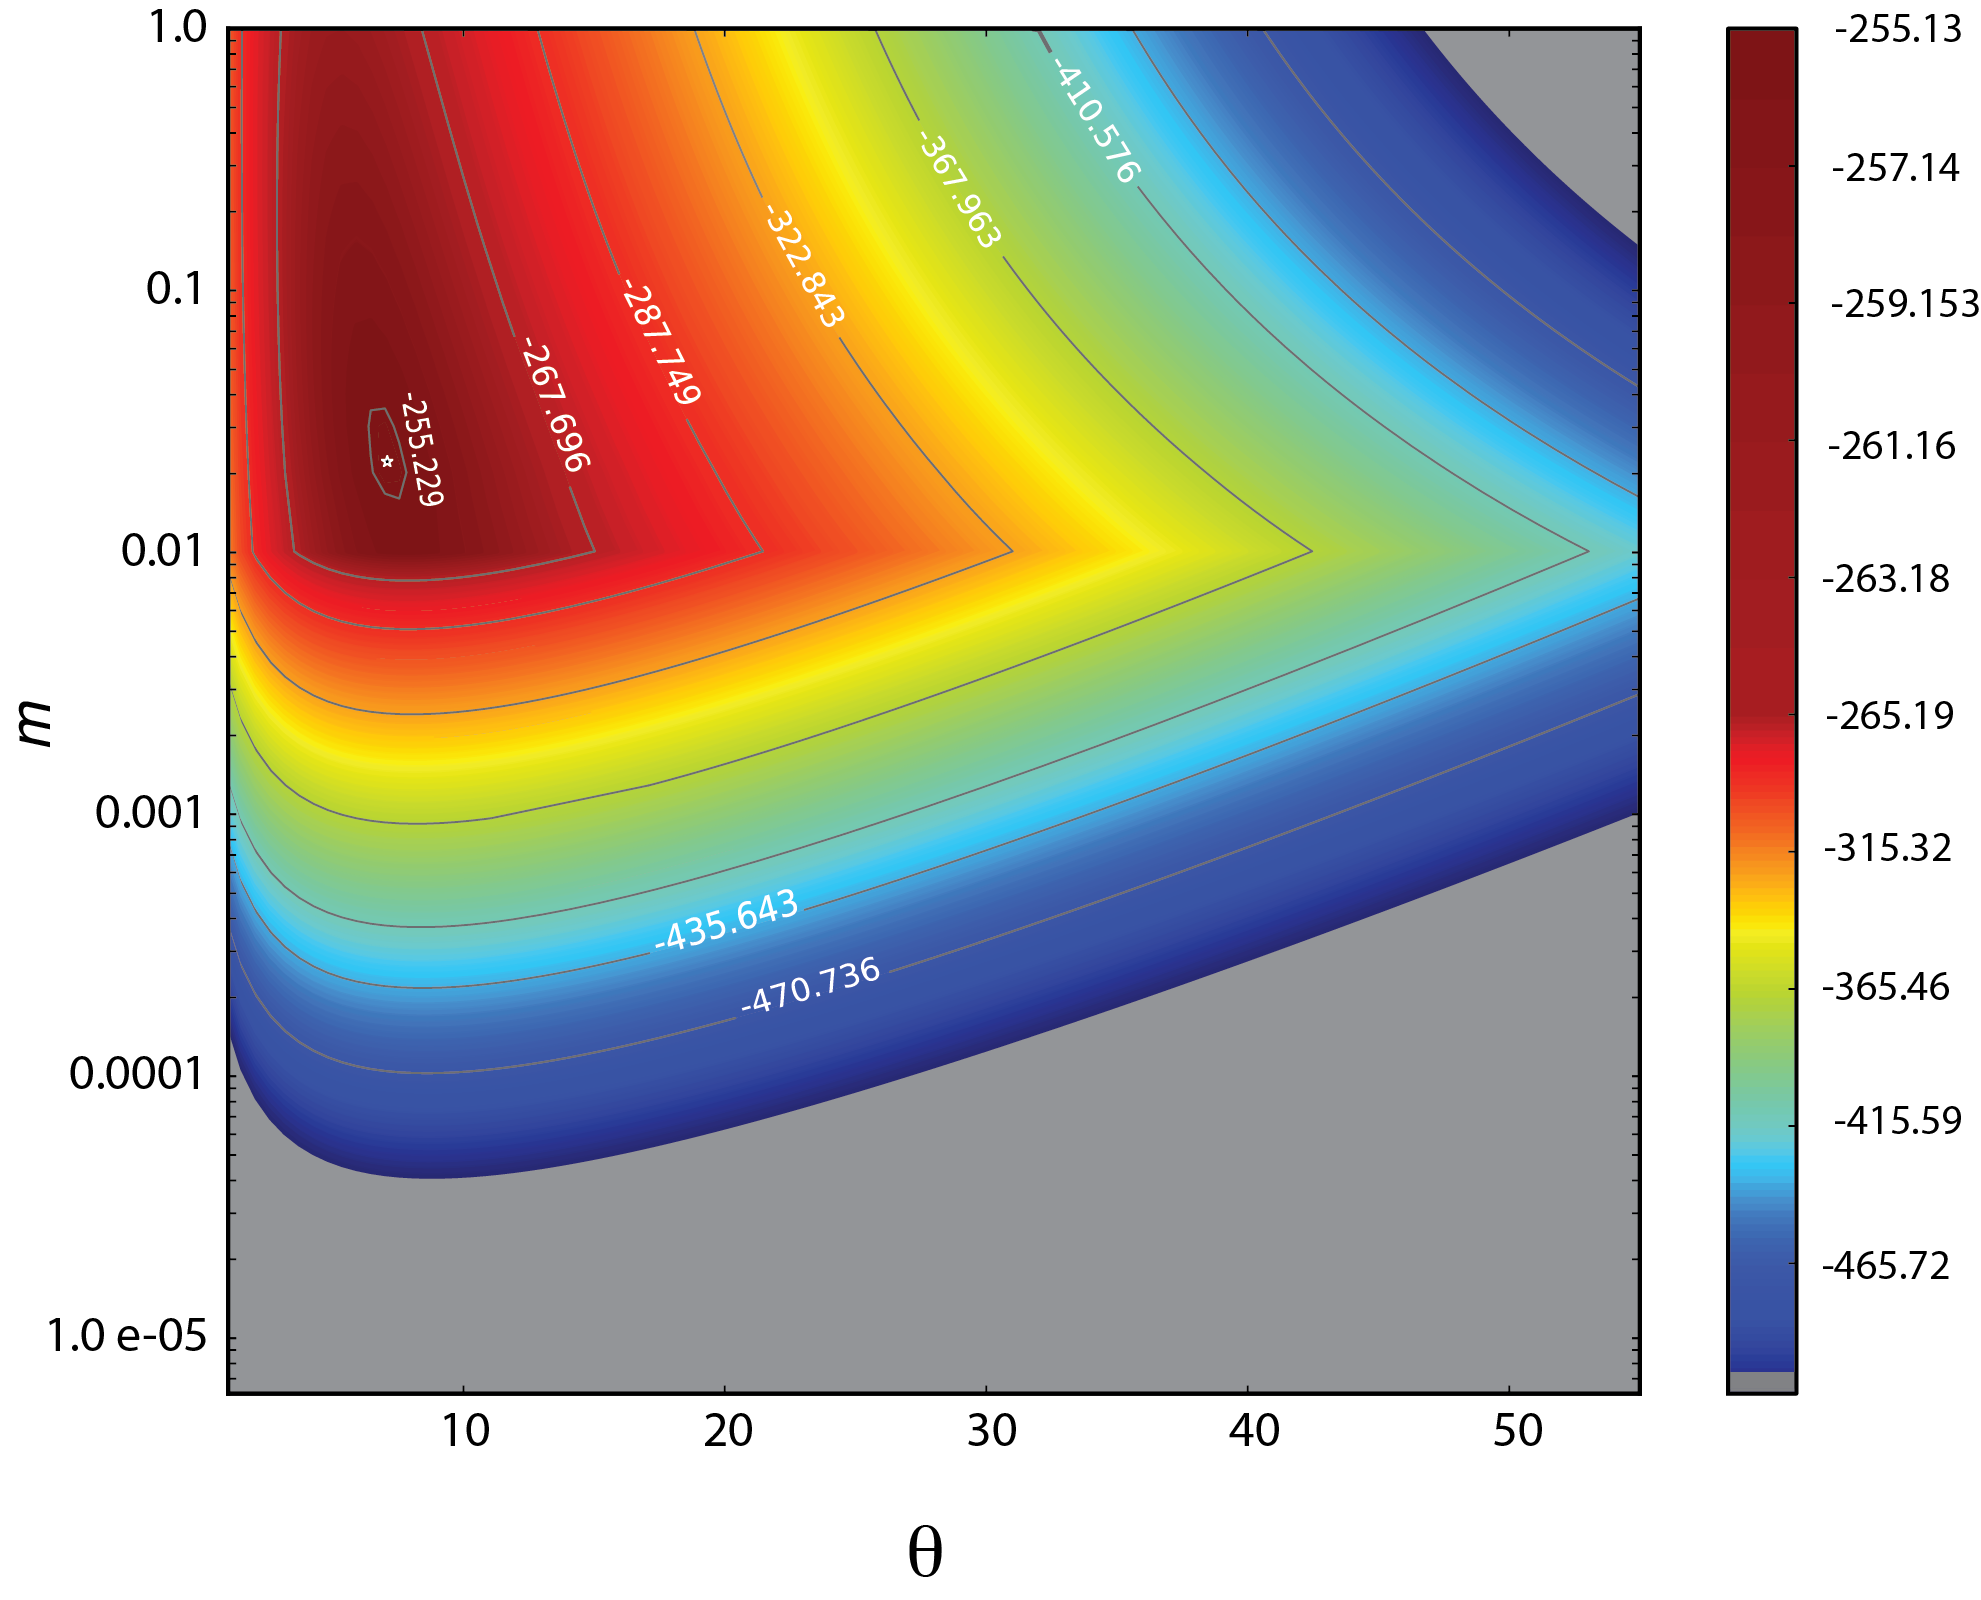
\includegraphics[width=\textwidth]{tex_source/figures/untb_genomes/lnl_chrom.png}
\caption[Maximum likelihood inference of neutral parameters.]{{\bf Maximum likelihood inference of neutral parameters.}\\ Log likelihood surface as a function of migration rate ($m$), and the fundamental biodiversity number ($\theta$) for \textit{D. rerio} chromosome 19. Dark red color shows regions of the surface where parameters maximize the probability to explain abundances and diversity of genetic elements in the chromosome. Likelihood ratio tests favored Etienne in contrast to Ewens sampling formula to explain the observed data in the chromosome.}
\label{fig:lnl_chrom}
\end{figure}

\subsection{Model testing}

In order to compare and test the fit of the two models computed, a likelihood ratio test \cite{Wilks1938} was conducted thanks to the fact that Etienne's model is nested into Ewens'. Etienne's model has two free parameters while Ewens' only one (under this model $m$ parameter is fixed to 1), thus the number of degrees of freedom for the chi-squared distribution is 1.

Additionally, given the large number of test performed, statistical significances were corrected by false discovery rate (FDR) \cite{Benjamini2001}. Etienne's model was thus kept as best fit model for only those chromosomes that pass the LRT after FDR adjustment, otherwise the null model using Ewens' formula was selected.

\subsection{Test for neutrality}

In the last years two exact tests were developed in order to accept or reject the neutrality of a given community. Both tests are based on the comparison of a given number of random neutral community generated using the parameters estimated (see \ref{sec:model-optimization}) for the real data under neutrality. The comparison of the random neutral communities with the observed distribution of abundances, is the key point to test for neutrality.

The first of these tests \cite{Etienne2007} consists in comparing the distribution of likelihoods of fitting neutral model. This corresponding distribution of random neutral abundances is compared to the likelihood of the observed data. The major problem of this test is technical, the computation time needed to optimize the parameters of each abundance distribution and get the likelihoods is unrealistically too high when dealing with genomic elements.

The second test \cite{Jabot2011} uses, instead of likelihood, the comparison of Shannon's entropy, and is much faster as random neutral abundances do not need to be fitted into a neutral model.

Thus, from the neutral parameters obtained for each chromosome, we simulated distribution of abundances of genetic elements 10,000 times. 

To test for the UNTB the evenness of each simulated distribution was computed using the Shannon's entropy H \cite{Jabot2011}. The set of H values conform the neutral null distribution to test if the empirical H of chromosomes is beyond the expected by random \fref{fig:shannon_distrib}{}.


\begin{figure}[htpb]
\centering 
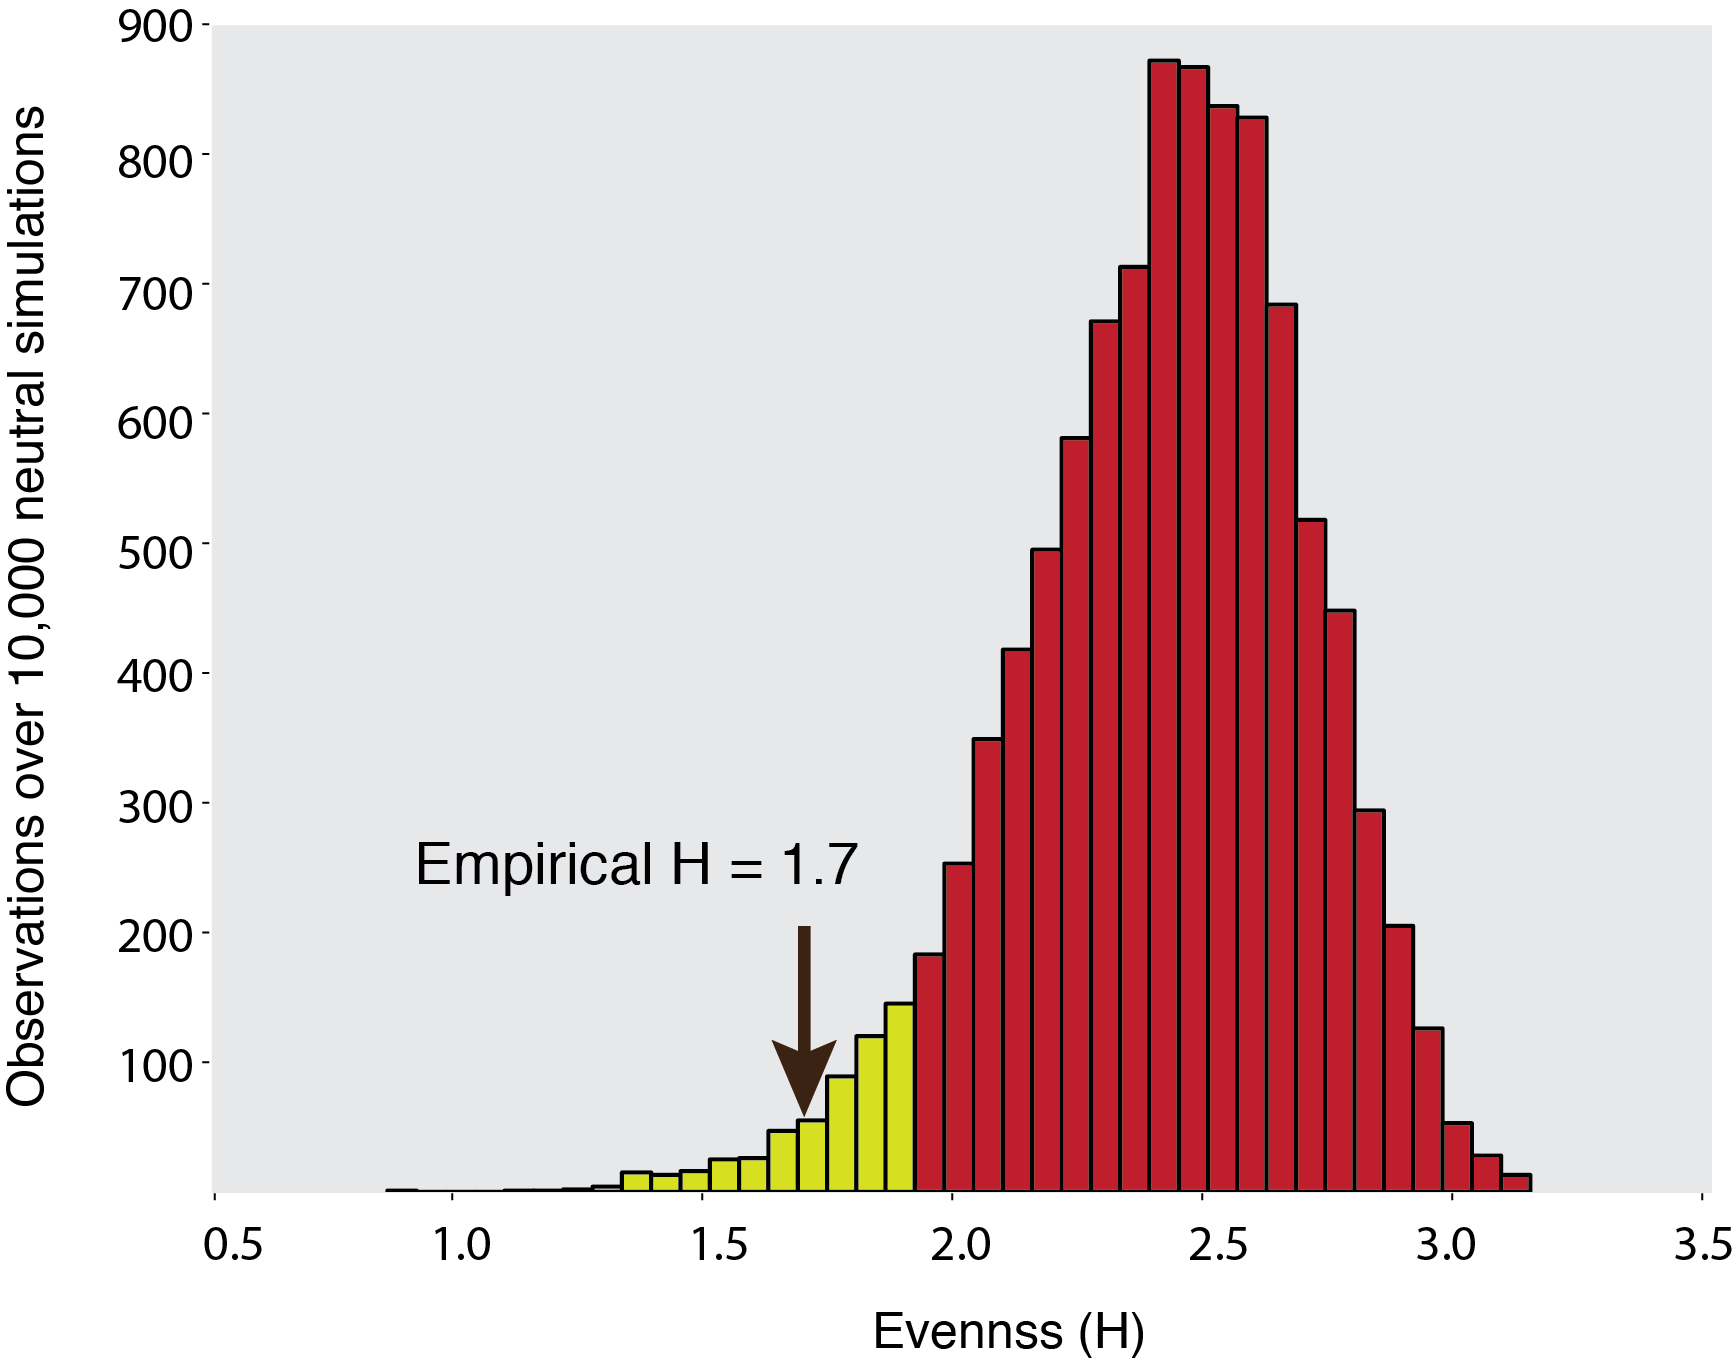
\includegraphics[width=\textwidth]{tex_source/figures/untb_genomes/shannon_distrib.png}
\caption[Comparing simulated and empirical evenness.]{{\bf Comparing simulated and empirical evenness. }\\Neutrality test statistically compares simulated null distribution of H with the empirical H value of the corresponding chromosome. In this case, the null distribution of H values was derived from 10,000 neutral simulations of A. gambiae chromosome 2L, with neutral parameters ($\theta$ and $m$) optimized by ML using Etienne sampling formulae. Yellow and red bars display 5\% and 95\% of the simulated neutral data, respectively. Although in this case neutrality was rejected (p= 0.01), posterior correction by multiple testing favored the null neutral hypothesis (q= 0.21).}
\label{fig:shannon_distrib}
\end{figure}



%%% Local Variables: 
%%% mode: latex
%%% TeX-master: "../../master"
%%% End: 


\part{Detection of selective pressures in genomes}
\chapter{Searching for evolutionary patterns in funcionally
  linked group of genes}
\label{chap:gssa}
%%% gssa.tex --- 


\section{Background}

In past years, with the development of genomic data in close related species, an effort was made in order to detect signals of selective pressure by applying methods that have been developed since \cite{Kimura1985} based on observations of significant deviation from neutrality for a given gene. These methodologies conceived for the study of a single gene were successfully able to detect genes escaping neutrality ($\omega \ne 1$ see Equation \ref{eq:omega} page \pageref{eq:omega}), and in particular positively selected genes (with $\omega > 1$)  \cite{Arbiza2006,Bakewell2007,Bustamante2005,Clark2003,Nielsen2005}. However none of those works were able to find, within the groups of genes detected to be under positive selection, a significant enrichment of a given functional trait. It is true that taking all those results together, assiduous readers could perceive functional patterns raising from all those studies. Functional terms related to \textit{Sensory perception}, \textit{Immune response} or \textit{Regulation of transcription} were present in almost all genomic studies of positive selection conducted in primates or rodents.


measured in coding regions using the  Statistical methods to test for neutrality \cite{Nielsen2001}, are currently used without considering if genes works independently or associated to others to produce a single phenotypic response. In this sense we are applying pre-genomics concepts and methods to genomics data. The current paradigm for large scale analysis of adaptation consists in a two steps framework: first, the search for a list of genes (in a gene-by-gene framework analysis) with a statistical significant signal of positive selection ($\omega > 1$), and second, the search for over-represented functional classes of genes in this list. Although it is logically consistent, it has been noted that this kind of strategy causes an enormous loss of information due to the large number of false negatives that are accepted in order to preserve a low ratio of false positives necessary when genomics data is considered~\cite{Al-Shahrour2007,Al-Shahrour2005a,Al-Shahrour2006,Subramanian2005}.

Genes do not operate alone within the cell, but in a intricate network of interactions that we have only recently started to envisage~\cite{Stelzl2005}. It is a widely accepted fact that coexpressing genes tend to be fulfilling common roles in the cell~\cite{Lee2003}. Moreover, coexpression seems to occur, in many cases, in contiguous chromosomal regions~\cite{Caron2001} and furthermore, recent evidences suggest that functionally related genes map close in the genome, even in higher eukaryotes~\cite{Hurst2004}. Many higher-order levels of interaction are continuously being discovered and even complex traits, including diseases, have started to be considered from a systems biology perspective~\cite{Ideker2008,Vamathevan2008}.

Recent methodology was proposed to circumvent the classical two-step analysis as a new attempt to test for selective signatures across species at genome-scale level~\cite{Shapiro2008} Using the deviations of the expected rates of evolution for a large group of genes in a group of gamma proteobacteria, the authors conclude that the coherence of selective patterns suggests that the genomic landscape is organized into functional modules even at the level of natural selection.

The hypothesis we aim to test in this study is not about individual genes, but about functional classes. Mutations occur on single genes but natural selection acts on phenotypes by operating on whole sub-cellular systems. Mutations in genes either remain finally fixed or disappear because of their beneficial or disadvantageous effect on individual fitness, respectively. This effect on the function of individual proteins can only be understood in the context of the system (e.g. a pathway, GO functional roles, etc.) in which the proteins are involved. If a list of genes arranged by some parameter that accounts for their evolutionary rates is examined, it is expected that genes belonging to pathways or functional classes favored or disfavored by selection will tend to appear towards the extremes.

This approach circumvents the implicit assumption posed by the two-step analysis described above assuming by that the gene is the only target of selection. If natural selection works by means of minor quantitative effects of many different changes distributed along different gene products most of them working together in a few number of systems (GO functional terms, biochemical pathways and/or interactome modules) we expect to find: \begin{inparaenum}[ 1-] \item correlated nonsynonymous rate changes associated to these functions , \item synonymous rate changes not necessarily associated to the same functions, \item a higher number of significant functions than those discovered in the classical two-step approach.\end{inparaenum}

In the first part of this paper we extend the classical two-step approach previously reported by us for human and chimp \cite{Arbiza2006}, to rat and mouse now considering a set of XXXX orthologous genes of human, chimpanzee, mouse, rat and dog. The objective is to compare the classical two-step approach with the new system approach developed in the second part of the paper. In both cases we search for differences in evolutionary rates differentiating positive selection from relaxation along the branches of the phylogeny of the species.

\section{Results}

\subsection{Gene-set selection analysis on functional modules}

Mammals, represented by human, chimpanzee, rat and mouse, and five Drosophila genomes were studied. For each species, genes were ranked into four lists according to the estimation of \begin{inparaenum}[i\upshape-] \item synonymous (dS), \item nonsynonymous (dN) rates of substitution, \item selective pressures ($\omega$ = dN/dS), and \item the change of selective pressures between (A) ancestor and (D) descendant species ($\Delta\omega$D = $\omega$D-$\omega$A) along the phylogeny \fref{fig:phylogeny}{}\end{inparaenum}. Maximum likelihood (ML) estimates of evolutionary variables were performed using a free-ratio branch model \cite{Yang2007}. As such, four lists containing 12,543 and 9,240 orthologous genes in mammals in Drosophila species were obtained for the analyzes, respectively. GSSA was conducted using a total of 1,394/199 and 1,331/116 GO/KEGG terms in mammals and Drosophila species respectively. GSSA is performed in five different steps (S1 to S5 in \fref{fig:gssa_met}{} on page \pageref{fig:gssa_met} in Section \ref{sec:gssa_mat-met}). First, the method ranks all genes within a genome (G) according to one of the alternative evolutionary variables (dS, dN, $\omega$ and $\Delta\omega$). Second, genes are associated (dark dots) to different functional categories (GO or any other functional term). Note that a single gene can be associated with multiple functions (yellow bar in Figure 2). Third, for each functional category a total of 30 partitions are established along the list of ranked values \cite{Al-Shahrour2007}, \cite{Al-Shahrour2005a}. Fourth, for each partition GSSA computes a two-tailed Fisher's exact test and reports significant over or under represented functional classes comparing the upper side (A) and the lower side (B) of the list. Finally, p-values are corrected for multiple testing (FDR). Throughout the manuscript only p-values for partitions with the highest confidence were reported after FDR.

The application of GSSA to lists of genes ranked by dS, dN, $\omega$ and the $\Delta\omega$ values yielded a large number of functional modules (defined by GO and KEGG annotations) with rates that were significantly skewed toward the extremes of the lists (\tref{tab:gssanum_perc}) in mammal and \textit{Drosophila} species. For instance, 11\% of GO terms, and 15\% of KEGG pathways contain genes with biased distribution of rates towards the top of the ranked list, and found statistically significant at high $\omega$ ratio (SH$\omega$, 5\% false-discovery rate, FDR) in mammals. Alternatively, 4.1\% and 2.6\% of GO terms and KEGG pathways were found with significantly high values of $\omega$ (SH$\omega$) in \textit{Drosophila}, respectively.

\begin{table}[htbp]
\begin{center}
\begin{tabular}{ l l l l l l }
\hline
 &  & \multicolumn{ 2}{c}{\textbf{SH*}} & \multicolumn{ 2}{c}{\textbf{SL*}} \\  \cline{ 3- 4} \cline{4-6}
 &  & \multicolumn{1}{c}{\textbf{KEGG }} & \multicolumn{1}{c}{\textbf{GO }} & \multicolumn{1}{c}{\textbf{KEGG }} & \multicolumn{1}{c}{\textbf{GO}} \\ \hline
\multicolumn{ 1}{l}{Mammals} &  dS  &  15 (1.9)    &  187 (3.3)   &  12 (2.1)    &  364 (6.5) \\
\multicolumn{ 1}{l}{} &  dN  &  145 (18.2)  &  708 (12.6)  &  230 (28.9)  &  1,839 (32.9) \\
\multicolumn{ 1}{l}{} & $\omega$ &  123 (15.5)  &  649 (11.6)  &  206 (25.9)  &  1,675 (30.0) \\
\multicolumn{ 1}{l}{} & $\Delta\omega$ &  64 (8.0)    &  421 (7.5)   &  107 (13.4)  &  818 (14.7) \\ \hline
\multicolumn{ 1}{l}{Drosophilas} &  dS  &  18 (3.1)    &  104 (1.5)   &  26 (4.5)    &  1,263 (18.9) \\
\multicolumn{ 1}{l}{} &  dN  &  31 (5.3)    &  276 (4.1)   &  26 (4.5)    &  2,097 (31.5) \\
\multicolumn{ 1}{l}{} & $\omega$ &  15 (2.6)    &  213 (4.1)   &  24 (4.1)    &  1,321 (19.8) \\
\multicolumn{ 1}{l}{} & $\Delta\omega$ &  2 (0.3)     &  143 (2.1)   &  7 (1.2)     &  184 (2.8) \\ \hline
\end{tabular}
\end{center}
\caption[Numbers and percentages of functional modules with significant results after GSSA.]{Numbers and percentages of functional modules with significant results after GSSA. For Significantly High (SH) and Significantly Low (SL) results.}
\label{tab:gssanum_perc}
\end{table}

\tref{tab:gssanum_perc} also reveals that functional modules with genes changing at significantly low $\omega$ ratios (SL$\omega$), and therefore showing a distribution shifted towards the bottom of the ranked list (see Figure 2), were more frequent than modules under the significantly high $\omega$ (SH$\omega$). This observation is in agreement with the fact that purifying selection is the predominant form of selection in biological systems. Moreover, in support of the slightly neutral character of synonymous mutations, and the effects of population size in the final outcome of selection \cite{Lynch2007} GSSA results show a higher number of significant deviations of dS in \textit{Drosophila} rather than in mammals.

Only a minor proportion of functional terms changed significantly at higher or lower rates relative to estimates of the corresponding ancestral lineages. Specifically, increased or decreased $\omega$ values on the external branches (recorded by positive and negative values of $\Delta\omega$) were observed for only half of the cases where a significant increase or decrease of $\omega$ was identified in mammals and Drosophilas. This observation points out the conservative character of the selective constraints in functional related groups of genes during evolution.

A summary of the results of the GSSA for mammals and \textit{Drosophilas} is shown in \fref{fig:tab_gssa}{} (see Figures S1 to S4 for a complete description of results after GSSA in mammals and \textit{Drosophila} species). The figure shows that GSSA has the power to detect many functional changes in evolutionary rates within a substantial number of functional categories. Although the rough pattern shows similar evolutionary constraints in groups of genes between the two main clusters of species, important differences were also detected within them. For instance, functional terms associated to neurological process and sensory perception clearly contrasted between primates and rodents (\fref{fig:tab_gssa}{-A}). While most of these terms are associated to a significant relative increase in rates from the common ancestor of primates (+$\Delta\omega$), all the changes observed in rodents were due to the relative increase of the selective constraints (-$\Delta\omega$) probably due to the effects of purifying selection from the common ancestor. Alternatively, functional modules associated to Immunity and Defense response evolved at significantly higher rates than expected in rodents, but decreased significantly in relation to the ancestral rates in primates. Such functional differences between primates and rodents were previously observed when pooling groups of species \cite{Kosiol2008a}. Other functional modules such as \textit{Development}, and \textit{Transcription/Transduction} comparatively evolved at very low dN and $\omega$ ratio but experienced a higher relaxation of the ancestral constraints (+$\Delta\omega$) in primates than in rodents. Moreover, significant differences in rates can be detected between human and chimpanzee (Ha04360: \textit{Axon guidance}, Ha04610: \textit{Antigen processes and presentation}, GO0007268: \textit{synaptic transmission}, among others), and between mouse and rat (GO0007186: \textit{G-protein coupled receptor protein signaling pathway}, and Ha04310: \textit{Wnt signaling pathway}, among others).


\begin{FPfigure}
\centering 
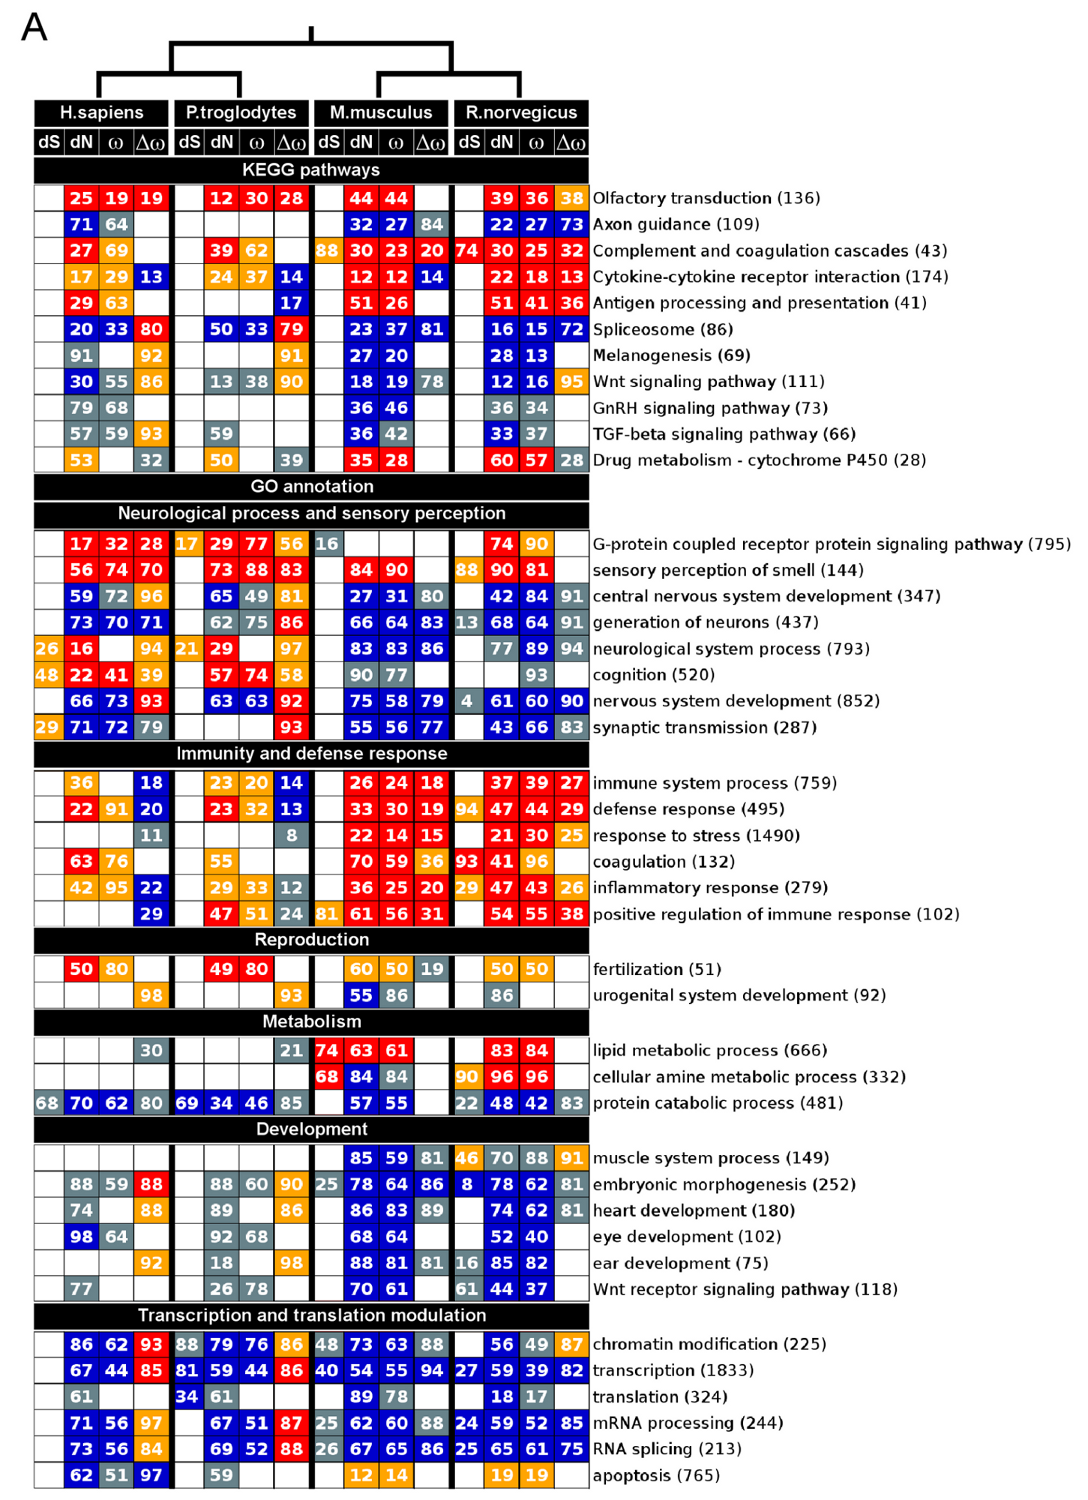
\includegraphics[width=\textwidth]{tex_source/figures/gssa/table_mammals_2.png}
\caption[GSSA of evolutionary variables.]{{\bf GSSA of evolutionary variables.} \\The figure shows a selection of GO terms and KEGG pathways with significant and not significant deviations after GSSA of evolutionary rates in mammals (A) and Drosophila (B) species. Colored boxes represent functional modules with genes significantly accumulated at the corresponding extremes of the ranked list as explained in Figure 2. The number inside each box represents the percentage of the total number of genes of the functional module (in parenthesis) that contribute to its significance. Here we reported the numbers of the first significant partition after FET and FDR. Topologies represent the phylogenetic relationships of species.} 
\label{fig:tab_gssa}
\end{FPfigure}
\begin{figure}
\centering 
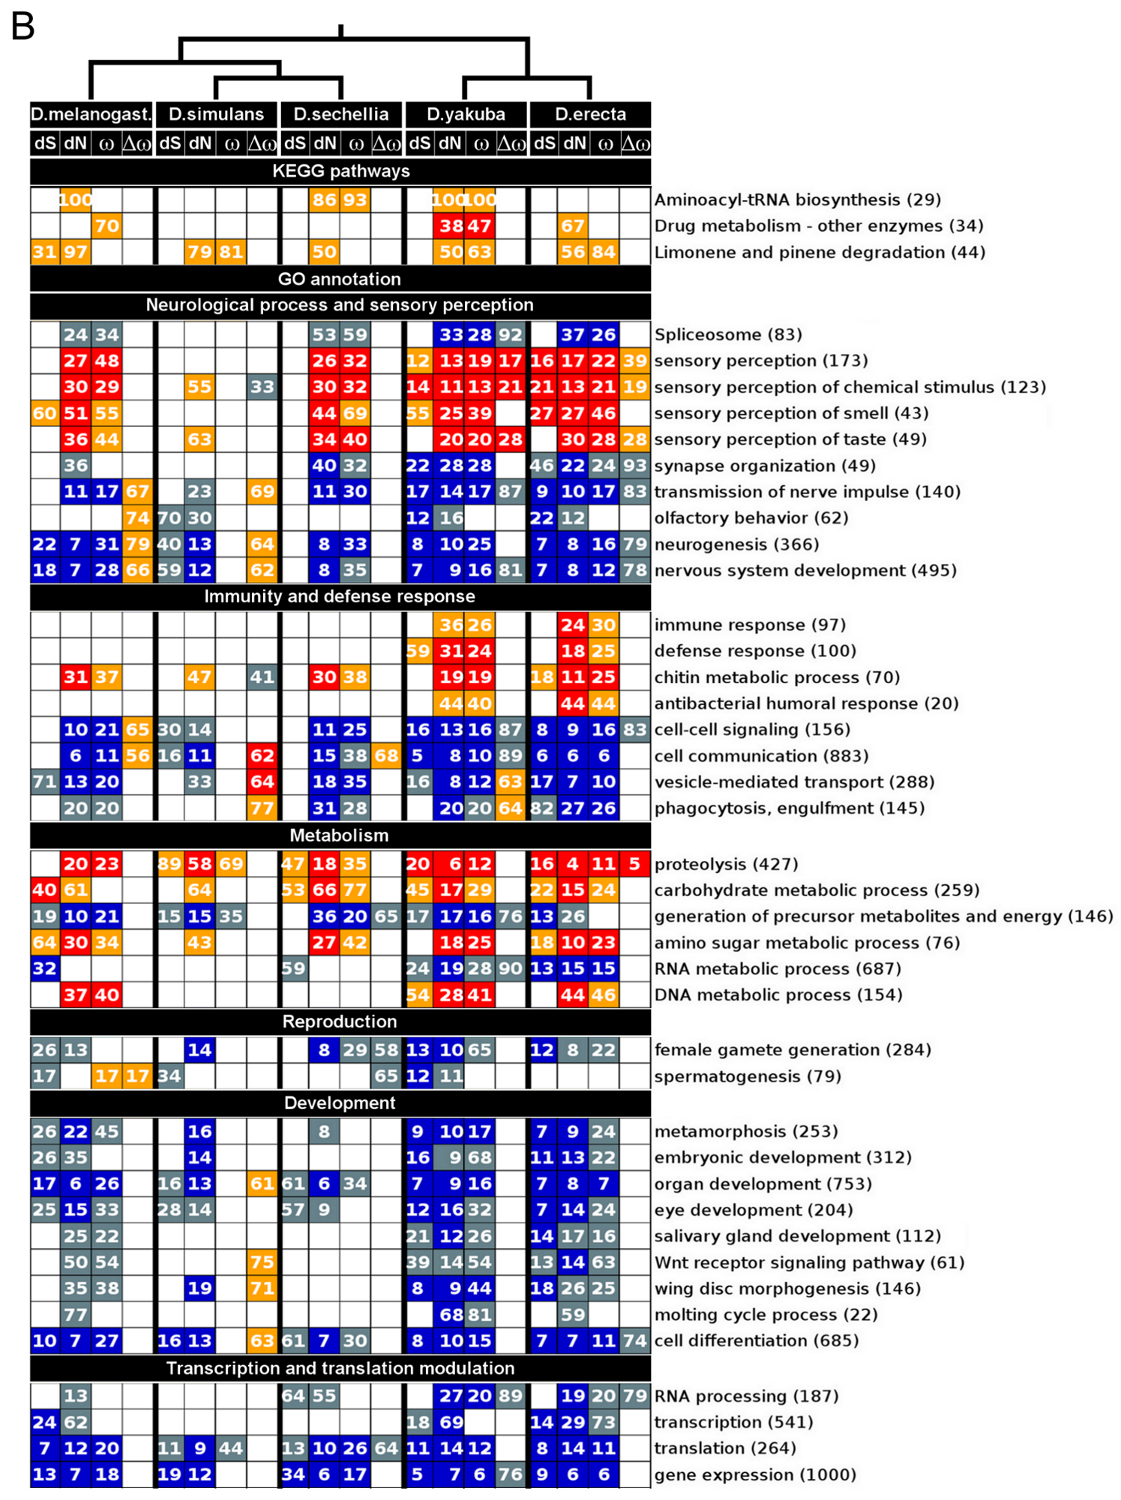
\includegraphics[width=\textwidth]{tex_source/figures/gssa/table_flies_2.png}
\end{figure}

<<<<<<< HEAD
In addition, most of the GO terms significantly associated to high dN and $\omega$ in  Drosophilas were unevenly distributed within the two clusters of the phylogeny (\fref{fig:tab_gssa}{-B}). GO terms such as sensory perception, defense response, immune response and metabolic process, among others, presented a remarkable divergence in the monophyletic groups of \textit{D. erecta} and \textit{D. yakuba} but they were not observed in \textit{D. sechellia}, \textit{D. melanogaster} and \textit{D. simulans}. Most of GO terms from \textit{Development}, \textit{Transcription} and \textit{Translation} (\fref{fig:tab_gssa}{-A and -B}) were significantly accumulated towards the extremes of the lists corresponding to the lowest rates of substitutions, suggesting they are significantly constrained by strong purifying selection (5\% FDR) in both taxa.
=======
In addition, most of the GO terms significantly associated to high dN and $\omega$ in Drosophilas were unevenly distributed within the two clusters of the phylogeny (\fref{fig:tab_gssa}{-B}). GO terms such as sensory perception, defense response, immune response and metabolic process, among others, presented a remarkable divergence in the monophyletic groups of \textit{D. erecta} and \textit{D. yakuba} but they were not observed in \textit{D. sechellia}, \textit{D. melanogaster} and \textit{D. simulans}. Most of GO terms from \textit{Development}, \textit{Transcription} and \textit{Translation} (\fref{fig:tab_gssa}{-A and -B}) were significantly accumulated towards the extremes of the lists corresponding to the lowest rates of substitutions, suggesting they are significantly constrained by strong purifying selection (5\% FDR) in both taxa.
>>>>>>> 3c532d72b9e9d3ab000c074b1476487348b6bde6

The fact that most of the functional modules under selection (SH$\omega$ and SL$\omega$) correlate with changes in dN, suggests that selective pressures are mainly driven by nonsynonymous rather than by synonymous substitutions during evolution. Moreover, according to the expectation of the nearly neutral theory, a low but still considerable number of significant associations of functional modules to dS were found in \textit{Drosophila} (19.5\%) and rodents (11.3\%), while in primates (6.4\%), where population sizes are known to be smaller, the number of significant modules was smaller \cite{Petit2009}.

The strategy presented here lead to detect significant patterns of increments and decrements modeled by natural selection in evolutionary rates of functional groups of genes. This pattern is consistent with the hypothesis that natural selection acts on phenotypes by the combined action of many functional related genes. Moreover, this functionally based approach identified with statistical significance, and on individual species, all the functional modules previously found significantly enriched by positively selected genes and therefore the main targets of adaptive biological functions in species \tref{tab:gssa_compare}. Although GSSA is not a test for positive selection, it is evident that functional modules containing PSGs can be significantly detected by this method on individual species. In the next section we will analyze the relative contribution of PSGs to the statistical differentiation of functional modules in genomes.


\rowcolors{2}{white}{gray}
\begin{FPtable}
\caption[Functional enrichment results using gene-by-gene and gene-set approaches.]{\textbf{Functional enrichment results using gene-by-gene and gene-set approaches.}\\The table depicts some selected biological functions enriched by PSGs as cited in references 1 to 7, and the corresponding significant result observed after GSSA of $\omega$ values. References 1 to 7 correspond to cites 6, 7, CSAC, 4, 5, 9 and 8 in the manuscript, respectively. Abbreviations: SHv: statistically significant high v values; SLv: statistically significant low v values; H: \textit{H. sapiens}; C: \textit{P. troglodytes}; Pr: primates; M: \textit{M. musculus}; R: \textit{R. norvegicus}; Ro: rodents; mel: \textit{D. melanogaster}; sim: \textit{D. simulans}; sec: \textit{D sechelia}; yak: \textit{D. yakuba}; ere: \textit{D. erecta}; Ds: \textit{Drosophila} species.\\
*: p=0.05;\\
** p=0.001. CSAC: Chimpanzee Sequencing and Analysis Consortium, Nature. 2005 vol. \textbf{437} (7055) pp. 69-87.}
\resizebox{410pt}{!}{%
  \begin{tabular}{ p{8.5cm} p{0.8cm} p{0.8cm} p{0.5cm} p{0.8cm} p{0.5cm} p{0.85cm} p{0.5cm} p{8cm}}
  \hline
  \textbf{Biological process} & \multicolumn{ 7}{c}{\textbf{Enrichment in PSGs}} & \textbf{GSSA: Functional category with significantly} \\ \hline
   & \textbf{1} & \textbf{2} &  \textbf{3} & \textbf{4} & \textbf{5} & \textbf{6} & \textbf{7} & \multicolumn{1}{r}{\textbf{HIGH rates of omega}} \\ \hline
  Olfaction/Sensory perception of smell & H & Pr** &  &  &  & Pr** &  & H**, C**, M**, R**, mel*, sec*, ere**, yak** \\
  Chemosensory perception & H & Pr** &  &  &  &  &  & H**, C**, M**, R**,  mel**, sec**, ere**, yak** \\
  G-protein-mediated signaling & H &  &  &  & H & Pr** &  & H**, C**, R* \\
  DNA/nucleic acid metabolism &  &  &  & C &  &  & Dr & C*, M**, R**, mel**, yak**, ere* \\
  Amino acid metabolism & H, C &  &  &  &  &  & Dr & M**, R** \\
  Proteolysis &  &  &  &  &  &  & Dr & M**, R**, mel**, sim*, sec*, yak**, ere** \\
  Fatty acid/Lipid metabolism &  &  &  &  & H &  & Dr & M**, R** \\
  Carbohydrate metabolism &  &  &  &  &  &  & Dr & sec*, yak*, ere* \\
  Adult reproduction and gametogenesis &  &  &  &  &  &  & Dr & sec* \\
  Spermatogenesis and motility &  & Pr* & Pr &  &  &  &  & H*, M*, mel* \\
  Immune response &  & Pr** &  & H, C &  & Ro** &  & C*, M**, R**, yak*, ere* \\
  Inflammatory response &  &  &  &  &  & Ro** &  & H*, C*, M**, R** \\
  Defense response &  &  &  &  &  & Ro** &  & H*, C*, M**, R**, yak**, ere* \\
  Response to wounding &  &  &  &  &  & Ro** &  & H*, M**, R** \\
  Hummoral imm. resp. mediated by circulating Ig &  &  &  &  &  & Ro** &  & M**, R** \\
  T-cell-mediated immunity &  & Pr** &  &  &  &  &  & M* \\
  Natural killer-cell-mediated immunity &  & Pr* &  &  &  &  &  & R* \\
  B-cell- and antibody-mediated immunity &  & Pr* &  &  &  &  &  & M**, R** \\
  Response to pest, pathogen, or parasite &  &  &  & H &  &  &  & C*, M**, R**, yak*, ere* \\
  Stress response &  &  &  &  & C & Ro** &  & M**, R** \\
  Response to external stimulus &  &  &  &  &  & Ro** &  & M**, R* \\
  Sensory Perception & H & Pr** &  & H &  & Pr** &  & H**, C**, M*, mel**, sec**, yak**. ere** \\
  Cell surface receptor-mediated signal trasnduction & H &  &  &  &  & Pr** &  & C* \\
  Cell adhesion & H &  &  &  &  &  &  & R* \\
  Amino acid transport &  &  & Pr &  &  &  &  & M* \\
  Protein amino acid glycosylation &  &  & Pr &  &  &  &  & M* \\
  Amino acid transport & C &  &  &  &  &  &  & M* \\ \hline
  \multicolumn{9}{r}{\textbf{LOW rates of omega}} \\ \hline
  Sensory Perception & H & Pr** &  & H &  & Pr** &  & R* \\
  Cell surface receptor-mediated signal trasnduction & H &  &  &  &  & Pr** &  & mel*, yak*, ere* \\
  Cell adhesion & H &  &  &  &  &  &  & H**, C**, mel**, ere* \\
  Amino acid transport &  &  & Pr &  &  &  &  & R* \\
  Protein amino acid glycosylation &  &  & Pr &  &  &  &  & H* \\
  Amino acid transport & C &  &  &  &  &  &  & C* \\
  Hearing / Perception of sound & H &  & Pr &  &  &  &  & M*, R* \\
  Neurological process &  &  &  &  &  & Pr** &  & M**, R**, yak*, ere* \\
  Synaptic transmission &  &  & Pr &  &  &  &  & H**, M**, R**, mel**, sec**, ere**, yak** \\
  Signal transduction/intracellular signaling cascade & H, C &  & Pr &  &  &  & Dr & H**, C**, M**, R**, dmel**, dsec*, dyak**, dere** \\
  Ion transport & H &  &  &  & H &  & Dr & H*, M**, R**, mel*, sec*, ere* \\
  Potassium ion transport &  &  & Pr &  &  &  &  & H*, C*, M**, R** \\
  Inorganic anion transport &  &  & Pr &  &  &  &  & M*, R* \\
  Intracellular protein traffic & H &  &  &  &  &  &  & H**, C**, M**, R**, mel*, sec**, yak**, ere* \\
  Transport &  &  &  &  &  &  & Dr & mel**, sec**, ere**, yak** \\
  Protein transport &  &  &  & H &  &  & Dr & H*, C**, M**, R**, mel**, sim*, sec**, ere**, yak** \\
  Metabolism of cyclic nucleotides & H &  &  &  &  &  &  & M*, R* \\
  Protein metabolism \& modification &  &  &  & H, C & C &  & Dr & H**, C**, M**, R**, ere*, yak* \\
  Phosphate metabolism/phosphorylation &  &  &  & H, C &  &  & Dr & H*, C*, M**, R**, mel*, sec**, yak**, ere* \\
  Purine metabolism & C &  &  &  &  &  &  & M*, R*, sec** \\
  Carbohydrate biosynthesis &  &  & Pr &  &  &  &  & M**, R* \\
  Cation transport & H &  &  &  &  &  &  & H*, M**, R** \\
  Nervous system development &  &  &  &  &  &  & Dr & H*, M**, R**, mel**, sec*, yak**, ere** \\
  Skeletal development & C &  &  &  &  &  &  & M**, R** \\
  Organ development &  &  &  &  &  &  & Dr & H*, M**, R**, mel**, sec*, yak**, ere** \\
  Post-embryonic development &  &  &  &  &  &  & Dr & M*, mel*, yak**, ere* \\
  Embryonic development &  &  &  &  &  &  & Dr & H**, C*, M**, R**, yak*, ere* \\
  Ectoderm development &  &  &  &  & H &  &  & C*, M*, R*, mel*, yak*, ere* \\
  Cell proliferation and differentiation & C &  &  &  &  &  & Dr & H**, C*, M**, R**, mel**, sec*, yak**, ere** \\
  Cell cycle &  &  &  &  &  &  & Dr & H*, M*, R*, mel**, sec**, yak**, ere** \\
  Cell structurre/morphogenesis & C &  &  &  &  &  & Dr & H**, C*, M**, R**, mel**, sec*, yak**, ere** \\
  Cell structure and motility & C &  &  &  &  &  &  & H*, M**, R**, sec* \\
  Inhibition of apoptosis &  & Pr* &  &  &  &  &  & H*, yak* \\
  Cell-cell signalling &  &  &  &  &  &  & Dr & H**, C*, M**, R**, mel**, sec**, ere**, yak** \\
  Regulation of nucleobase &  &  &  & H, C &  &  &  & H**, C**, M**, R**, ere* \\
  Translation &  &  &  &  &  &  & Dr & M*, R*, mel**, sim*, sec**, yak**, ere** \\
  Transcription &  &  &  & H, C & C &  & Dr & H**, C**, M**, R**, ere* \\
  Protein catabolism &  &  &  & H, C & C &  &  & H**, C**, M**, R** \\
  Interferon-mediated immunity &  & Pr* &  &  &  &  &  &  \\ \hline
  \end{tabular}
}
\label{tab:gssa_compare}
\end{FPtable}

\subsection{Positively selected genes and the evolution of functional modules}

GSSA tests for difference in rates over functional related groups of genes. To what extent genes under positive selection contribute to the significance of functional modules in mammals and \textit{Drosophila} species after GSSA? To answer this question, branch-site (the most sensitive) test of positive selection was conducted on terminal branches of phylogenies \ref{fig:phylogeny}{}. We found 715 PSGs in mammals and 626 in \textit{Drosophila}. \fref{fig:gssa_psgs}{-A} shows the distribution of the mean evolutionary rates (dN and dS) of functional modules providing significant and not significant results after GSSA of the $\omega$ ratio. When considering the total number of the functional modules with PSGs, 55\%, 53\%, and 42\% of these original functional categories observed with SH, SL and NS results after GSSA ($\omega$ values) still remained \fref{fig:gssa_psgs}{-B}. This suggests that: \begin{inparaenum}[1\upshape-]\item evolution of many of the functional modules changing at SH$\omega$ ratios in the genome is not driven by a considerable accumulation of PSGs. Functional modules such as \textit{complement and coagulation cascades} in human, \textit{gonad development} in chimpanzee, \textit{regulation of innate immune response} in mouse, \textit{primary immunodeficiency} in rat, and \textit{spermatid differentiation} in \textit{D. melanogaster} are examples of functional modules evolving at significantly elevated $\omega$ ratio without any PSGs; \item molecular adaptation takes place in functional modules under strong selective constraints (see last part of \tref{tab:gssa_compare}). For instance, \textit{apoptosis} in human, \textit{generation of neurons} in chimpanzee, \textit{tissue development} in mouse, \textit{Wnt signaling pathway} in rat, \textit{eye development} in \textit{D. melanogaster}, \textit{wing disc development} in \textit{D. yakuba}, and \textit{generation of neurons} in \textit{D. erecta} are some of the functional modules evolving at SL$\omega$ ratios in the corresponding genomes that contain PSGs; and finally, \item an important number of functional modules without significant differences in $\omega$ ratios (grey dots in \fref{fig:gssa_psgs}{}) still contain genes under positive selection. For instance, \textit{homologous recombination} in humans, brain \textit{development} in chimpanzee, \textit{female or male sex differentiation} in mouse, \textit{regulation of mitotic cell cycle} in rat, \textit{chromatin modification} in \textit{D. sechellia}, and \textit{oogenesis} in \textit{D. melanogaster}.\end{inparaenum} 

These results are in agreement with previous observations in \textit{Drosophila} were it was emphasized that not every mutation under positive selection responds to a change in selection \cite{Images2009}. Beneficial changes could occur at evolutionary equilibrium, repairing previous deleterious changes and restoring existing functions \cite{Images2009}.

\begin{FPfigure}
\centering 
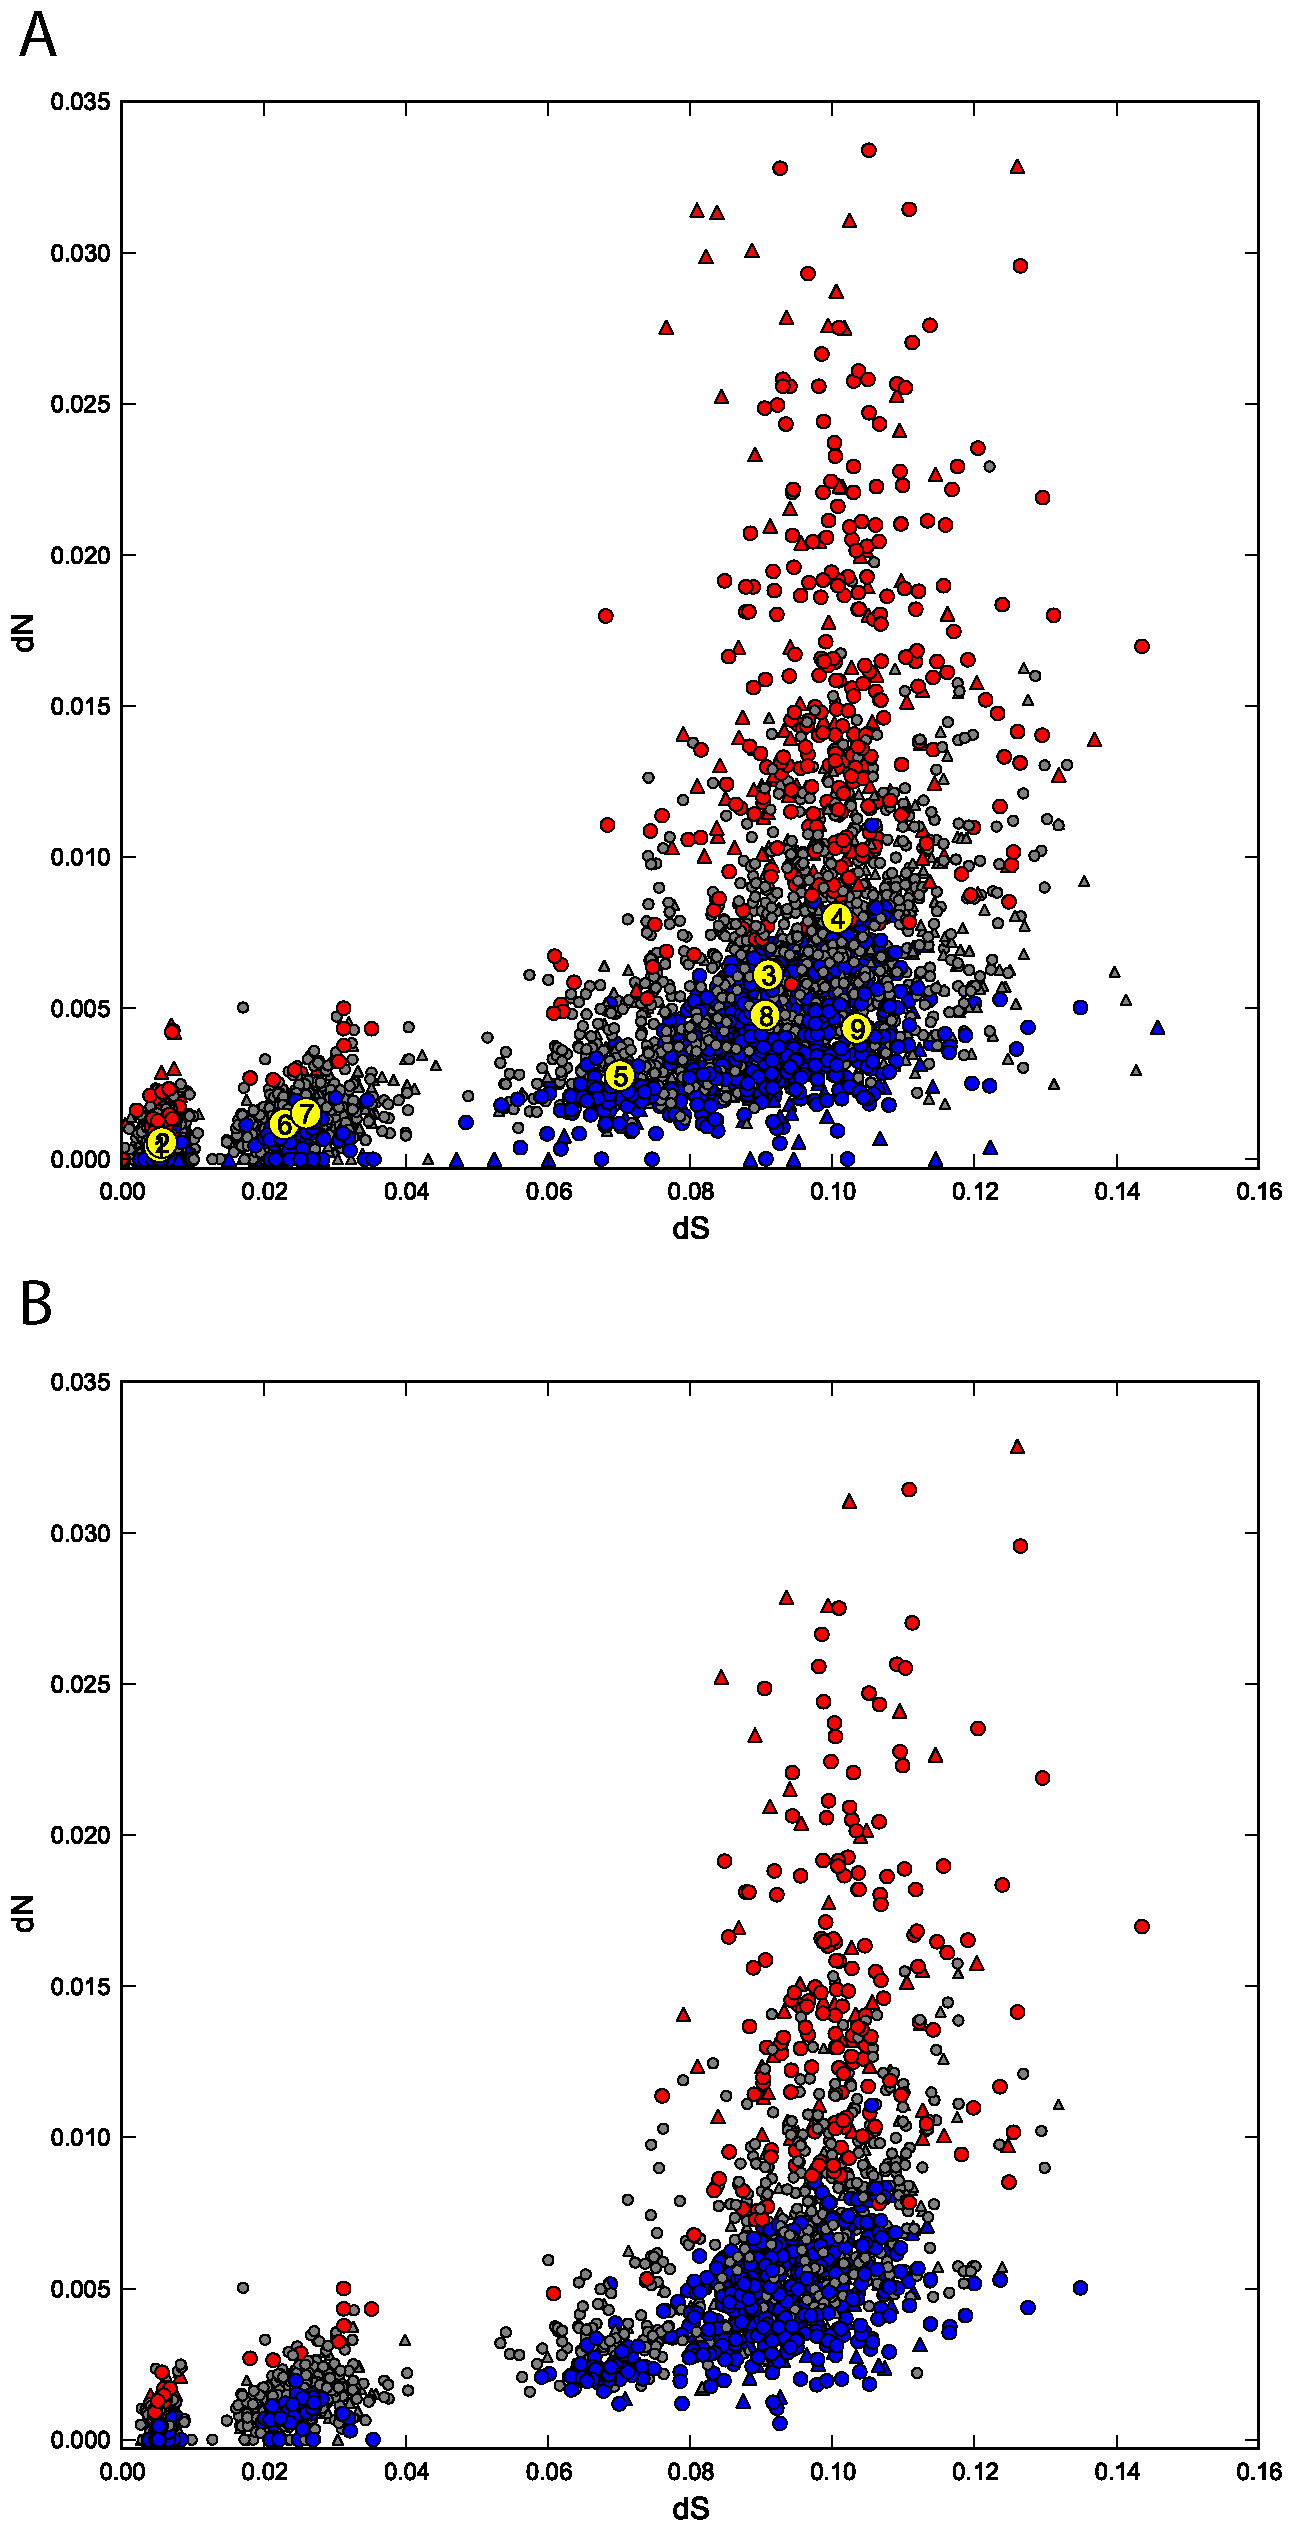
\includegraphics[height=\textheight]{tex_source/figures/gssa/gssa_psgs.png}
\caption[ Positive selection and evolution of functional modules.]{{\bf  Positive selection and evolution of functional modules.} \\Circles and triangles represent the median values of dN and dS for KEGG pathways and GO terms (level 6-7), respectively in mammals, and in the \textit{Drosophila} species. Functional modules with SH$\omega$ and SL$\omega$ results after GSSA are shown in red and blue. Those modules without statistical differences are gray. Yellow dots depict the median dS and dN values for \textit{H. sapiens} (1), \textit{P. troglodytes} (2), \textit{M. musculus} (3), \textit{R. norvegicus} (4), \textit{D. simulans} (5), \textit{D. sechellia} (6), \textit{D. melanogaster} (7), \textit{D. yakuba} (8) and \textit{D. erecta} (9). (B) In this case, circles and triangles represent a subset (of A) with modules containing at least one PSG. Note that they are distributed along a wide range of values of dS and dN and in functional categories with significant (red/blue), and non-significant (gray) results after the GSSA ($\omega$ ratio).} 
\label{fig:gssa_psgs}
\end{FPfigure}

Finally, we ask if PSGs preferentially concentrate in functional modules evolving at faster rates in different genomes. For doing that we computed the mean number of PSGs in functional modules with SH$\omega$ and SL$\omega$ results (red and blue dots in \fref{fig:gssa_psgs}{-B}. As expected, functional modules evolving at high $\omega$ ratio contain higher numbers of PSGs in rodents (p$<$0.001), mammals (p$<$0.001), and \textit{Drosophila} (p$<$0.001) species. For primates however, it was not significant (p = 0.47), indicating that PSGs are distributed almost evenly in functional modules evolving at significantly high and low values of $\omega$ in human and chimpanzee.

To contrast these results, PSGs from previous works in mammal and \textit{Drosophila} species were collected \cite{Clark2007}, \cite{Kosiol2008a}. The pattern of distribution of PSGs in functional modules was in agreement with the mentioned results: significantly skewed (p$<$0.001) towards higher numbers of PSGs in mammals, rodents, and \textit{Drosophila} species, but showing no differences in primates (p = 0.73).

In summary, PSGs are frequently observed in functional modules evolving under a wide range of evolutionary scenarios; however, they concentrate more frequently in functional groups of genes changing at elevated rates in rodents and \textit{Drosophila} species. Alternatively, PSGs were evenly distributed in functional modules changing at the extreme rates of evolution in primates. This observation suggests that a more complex scheme than the cumulative differences of PSGs must rely on the observed adaptive differences in human and chimpanzee genomes. The search for integrative factors taking into account the action of multiple genes other than only those which have been targeted by positive selection \cite{He2010}, could provide a more accurate view for the analysis of the integrated framework underlying adaptation in complete genomes.

\section{Material and Methods}
\label{sec:gssa_mat-met}
\subsection{Orthology prediction}

Complete genomes of 5 mammals species (\textit{Homo sapiens}, \textit{Pan troglodytes}, \textit{Mus musculus}, \textit{Rattus norvegicus} and \textit{Canis familiaris}) where retrieved from \textit{Ensembl} \cite{Flicek2011}. Also orthology prediction between each pair of species possibly done between human and the others was retrieved from \textit{Ensembl Compara} \cite{Vilella2009} using biomart \cite{Kinsella2011} and taking human as \gls{seed} species. Only groups of orthologs \textit{one-to-one} with one representative of each species where kept in the final dataset \fref{fig:phylogeny}{-A}.

\begin{figure}[htpb] 
\centering 
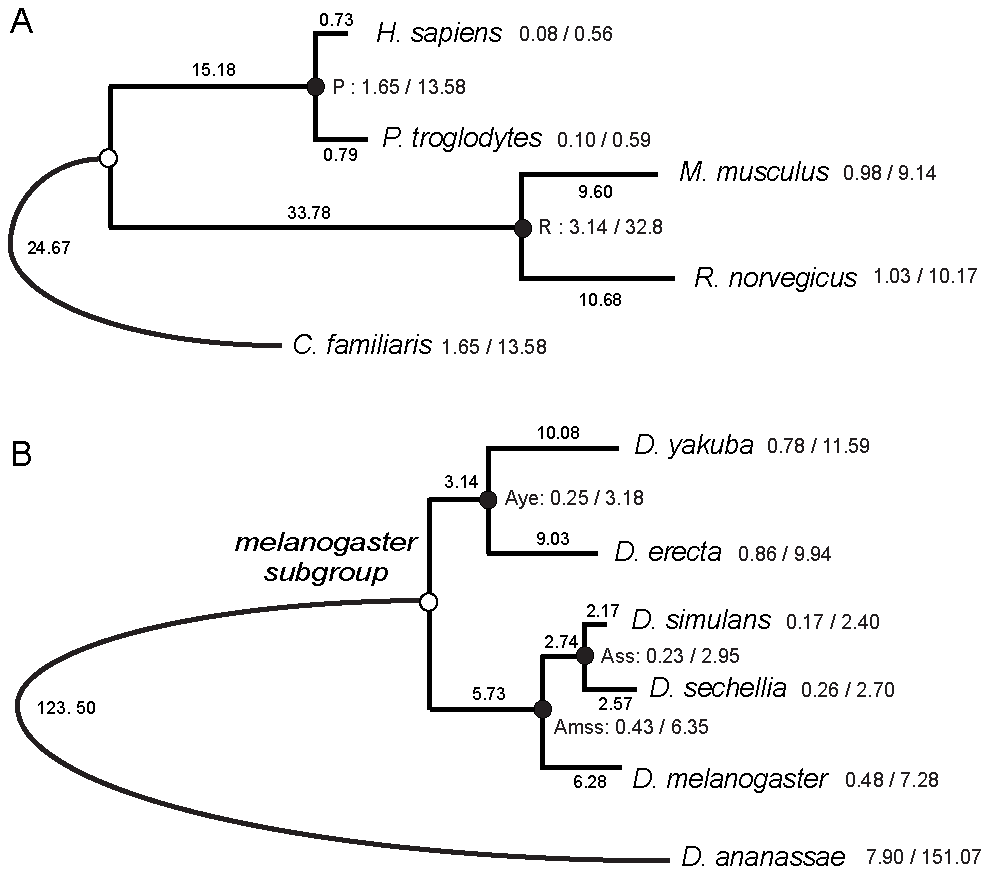
\includegraphics[width=\textwidth]{tex_source/figures/gssa/phylogenies.png}
\caption[Mammals and \textit{Drosophila} phylogeny]{{\bf Mammals and
 \textit{melanogaster} group phylogeny.} \\Numbers on internal and external nodes represent the median number of nonsynonymous and synonymous substitutions per codon (dN/dS) estimated from all the coding sequences compared in mammal (A) and Drosophila (B) genomes. Branch lengths and rates were multiplied by 100. Ancestral estimation of parameters was done in primates (P), rodents (R), D. yakuba and D. erecta (Aye), D. simulans and D. sechellia (Ass), and D. melanogaster, D. simulans and D. sechellia (Amss). C. familiaris and D. ananassae were chosen as outgroup species in the corresponding tree.} 
\label{fig:phylogeny}
\end{figure}


The same procedure was applied for \textit{melanogaster} group, including 6 species namely, \textit{Drosophila melanogaster} (as \gls{seed}-species), \textit{Drosophila sechelia}, \textit{Drosophila simulans}, \textit{Drosophila yakuba}, \textit{Drosophila erecta} and, as outgroup, \textit{Drosophila ananassae} (see \fref{fig:phylogeny}{-B}).

\subsection{Alignments refinement and filters}
DNA coding sequences (CDS) were aligned according to protein translation pattern using \textit{Muscle} version 3.7 \cite{Edgar2004} embedded into the \textit{CDS-Protal} utility in \textit{Phylemon 2.0} \cite{Sanchez2011}, and to avoid the presence of badly aligned regions alignments were cleaned using \textit{TrimAl} \cite{Capella-Gutierrez2009} keeping all sequences but trimming alignment columns with the heuristic method \textit{automated-1}. Additionally, alignments smaller than 100 bp were excluded from the analysis. 

In mammals, the upper limit for dN and dS considered was those of the human interferon $\gamma$ (dN = 3.06) and the relaxin protein \cite{Graur2000} (dS = 6.39 substitutions per site per 1e9 years). Assuming the human-mouse, mouse-rat and human-chimp differentiation times to be about 80, 70 and 5 million years \cite{BlairHedges2003}, respectively, ortholog comparisons between primates and rodents with dS$\ge$1 and dN$\ge$0.5, rodents with dS$\ge$0.256, dN$\ge$0.122, and primates with dS$\ge$0.064 and dN$\ge$0.030 substitutions/site were excluded.

The number of orthologs kept for analysis after filtering steps, is 12,453 for mammals, and 9,240 for flies.

\subsection{Evolutionary analysis}

Maximum likelihood estimation of dN, dS, and $\omega$ was computed using CodeML program from PAML \cite{Yang2007}. Evolutionary rates were computed in orthologous sequences according to the free-ratio branch model assuming independent $\omega$ ratio for each branch of the tree of mammals and Drosophila species (see raw values of rates in Table S1 and S2). Evolutionary rates (dN, dS), its ratio ($\omega$), and its difference between ancestral and descendant species ($\Delta\omega$) were ranked along all genes of genomes and further analyzed by GSSA.

External branches of Figure 1 were labeled as foreground to test for positive selection using branch-site models in Test I and Test II \cite{Zhang2005}. Positive results of relaxation of selective constraints (or weak signals of positive selection) were discarded \cite{Arbiza2006}. To quantify the relative contribution of PSGs in functional modules showing SH$\omega$ and SL$\omega$ results in GSSA, a t-test (from R package \cite{Ihaka1996}) with the mean number of PSGs per functional modules was computed in primates, rodents, mammals and Drosophila species. An independent set of PSGs was collected to test the robustness of our results in mammals \cite{Kosiol2008a}, and Drosophila species \cite{Clark2007}.

\subsection{GSSA, evolutionary and statistical simulations}

Gene-set selection analysis across lists of genes ranked by different evolutionary rate parameters (dS, dN, $\omega$ and $\Delta\omega$) was computed using the program Babelomics \cite{Al-Shahrour2008}. This program implements a version of GSA \cite{Al-Shahrour2005a} which can be applied to any list of ranked genes regardless of the initial experimental design \cite{Dopazo,Huang2009}. The aim of the test is to find functional classes, namely blocks of genes that share some functional property, showing a significant asymmetric distribution towards the extremes of a list of ranked genes. This is achieved by means of a segmentation test, which consists on the sequential application of a Fisher's exact test over the contingency tables formed with the two sides of different partitions (A and B in \fref{fig:gssa_met}) made on an ordered list of genes. The two-tailed Fisher's exact test finds significantly over or under represented functional classes when comparing the upper side to the lower side of the list, as defined by any partition (in \fref{fig:gssa_met}, four of the five partitions show significant differences). Similarly to other equivalent gene-set analyses, the outcomes are those modules (GO and KEGG) significantly associated to high or low values of the evolutionary parameter used to rank the genes. Previous results showed that a number between 20 and 50 partitions often gives optimal results in terms of sensitivity and results recovered \cite{Al-Shahrour2005a}. Here we applied 30 partitions along all the GSSA performed. Given that multiple functional classes (C) are tested in multiple partitions (P), the unadjusted p-values for a total of C $\cdot$ P tests were corrected by the widely accepted FDR method \cite{Benjamini2001}.

\begin{FPfigure}
\centering 
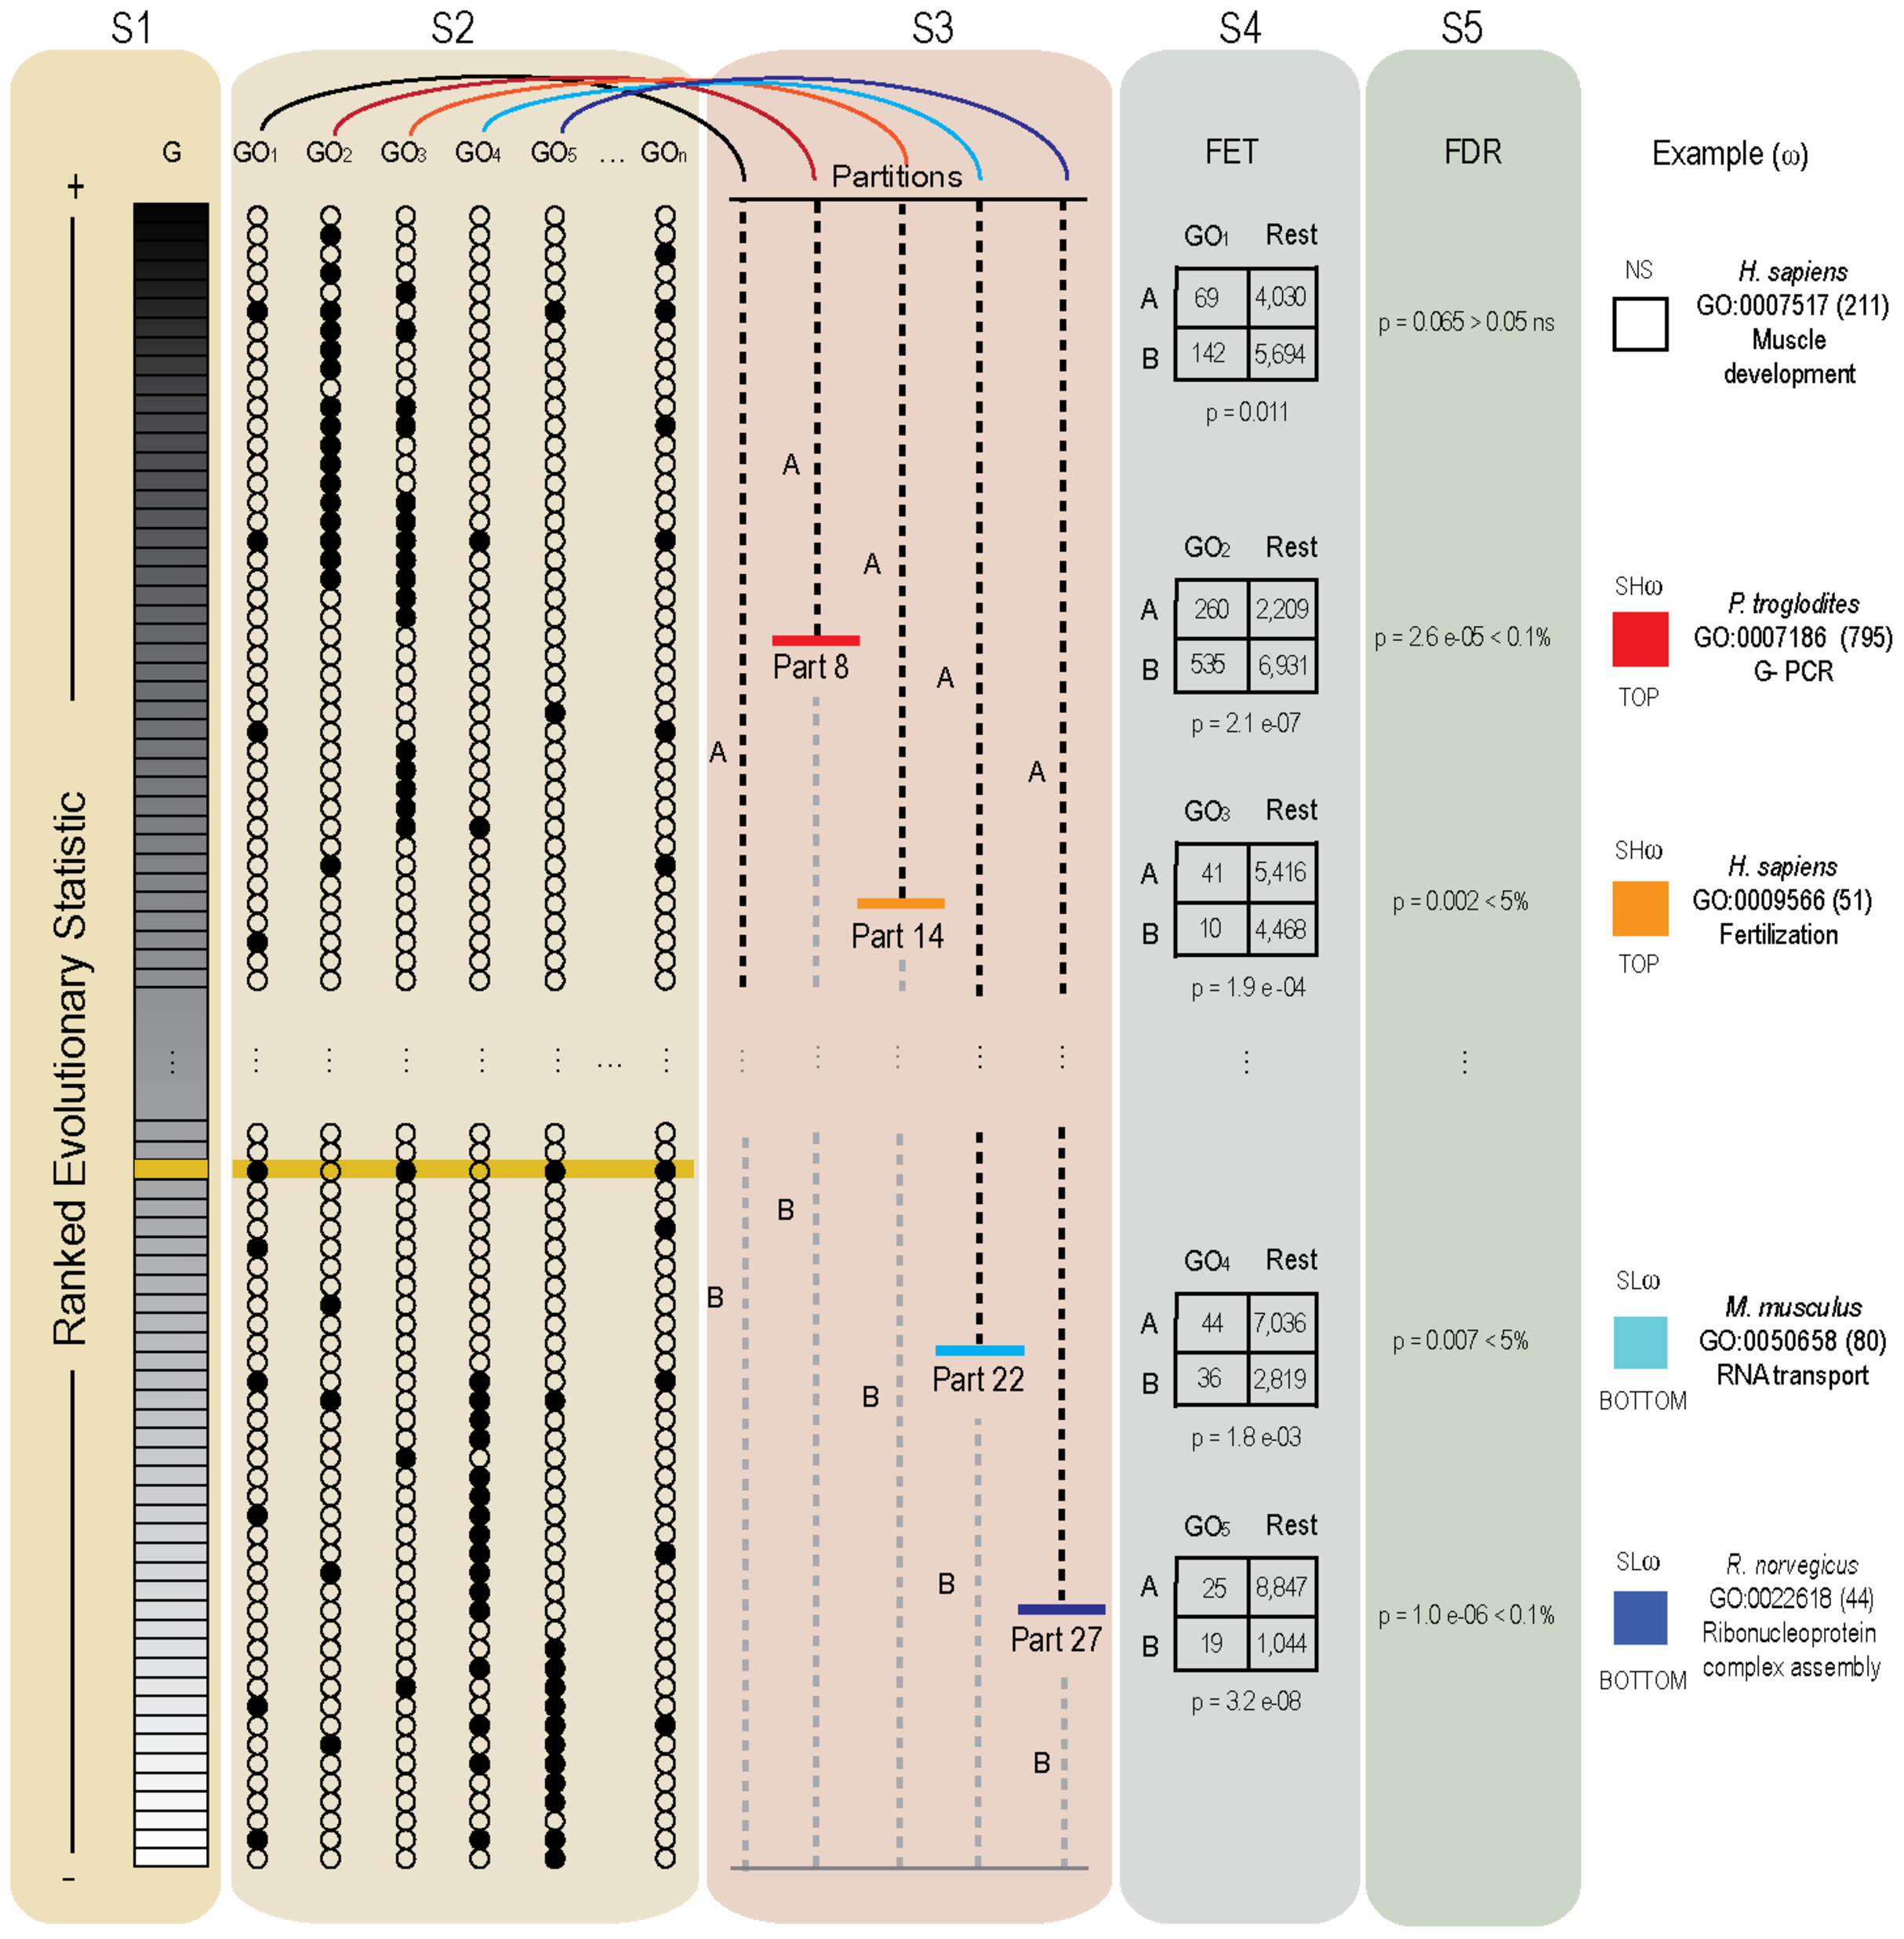
\includegraphics[width=\textwidth]{tex_source/figures/gssa/gssa_met.pdf}
\caption[Summary of the steps developed by the GSSA.]{{\bf Summary of the steps developed by the GSSA.} \\GSSA can be roughly described in a series of five steps (S1 to S5). S1: rank genes of a genome according to an evolutionary variable, S2: assign functional classes to all the listed genes, S3: apply a fixed number of partitions on the ranked list, S4: proceeds with a Fisher exact test (FET) for each partition, S5: adjust p-values by FDR. See text for a full description. Colored boxes (red, orange, cyan and blue) represent functional modules with genes significantly accumulated (0.1\% FDR and 5\% FDR) at the corresponding extremes of a list (top and bottom), and therefore with significantly high (SH) and low (SL) values of the evolutionary variable ($\omega$) respectively. White represents a non-significant association (NS). Examples show five alternative GO categories with significant and non-significant distributions of the $\omega$ statistic. In parenthesis, the total number of genes corresponding to the GO term is shown. For GO1, the function seems to be uncorrelated with the arrangements of the genes. In the example (GO:0007517) partition 16 in human (not shown in the picture) reported the lowest p-value (p = 0.011) although it was not significant after FDR correction (FDR = 0.065). Upper (A) and lower (B) sides of the ranked list (S3) represent both sides of the specified partition number. Remainder GO categories (GO2 to GO5) show the association of dark dots with values located at the top (significant high $\omega$ values -SH$\omega$), and at the bottom (significant low $\omega$ values -SL$\omega$) of the list (for GO2-GO3 and GO4-GO5, respectively). In examples, FETs found the most significant p-value for partitions 8, 14, 22 and 27 for GO:0007517, GO:0007186, GO:0009566, GO:0050658 and GO:0022618 in chimpanzee, human, mouse and rat genome, respectively.}
\label{fig:gssa_met}
\end{FPfigure}

Originally, 1,394/1,331 GO terms, and 199/116 KEGG pathways were analyzed in mammals and Drosophila species respectively. The global GO directed acyclic graph was processed with Blast2GO \cite{Conesa2005} to extend the annotation at missing parental nodes, discarding GO levels out of 2 to 8 for mammals, and 2 to 12 for Drosophilas. The final set of GO and KEGG terms used in the GSSA corresponds to those containing a minimum number of 15 genes. To test possible biases attributed to the size of the functional category, the magnitude of change in evolutionary rate or the proportion of genes experiencing a rate change we randomized the original assignation of ENSG's to the list of ranked values and functional annotation (see \fref{fig:gssa_simul}{-A}). For each evolutionary variable and species 10.000 randomizations and the corresponding GSSA were performed. The proportion of false positives (significant results after GSSA) was computed for each evolutionary variable and plotted along the size of functional categories (from 20 to 1,400 with intervals of 20). Because this proportion never reached values higher than 0.5\% (FDR) we rejected the possibility that either group size or rate distribution biased GSSA results in our data set (see \fref{fig:gssa_simul}{-B} and \fref{fig:gssa_simul}{-C}).

\begin{FPfigure}
\centering 
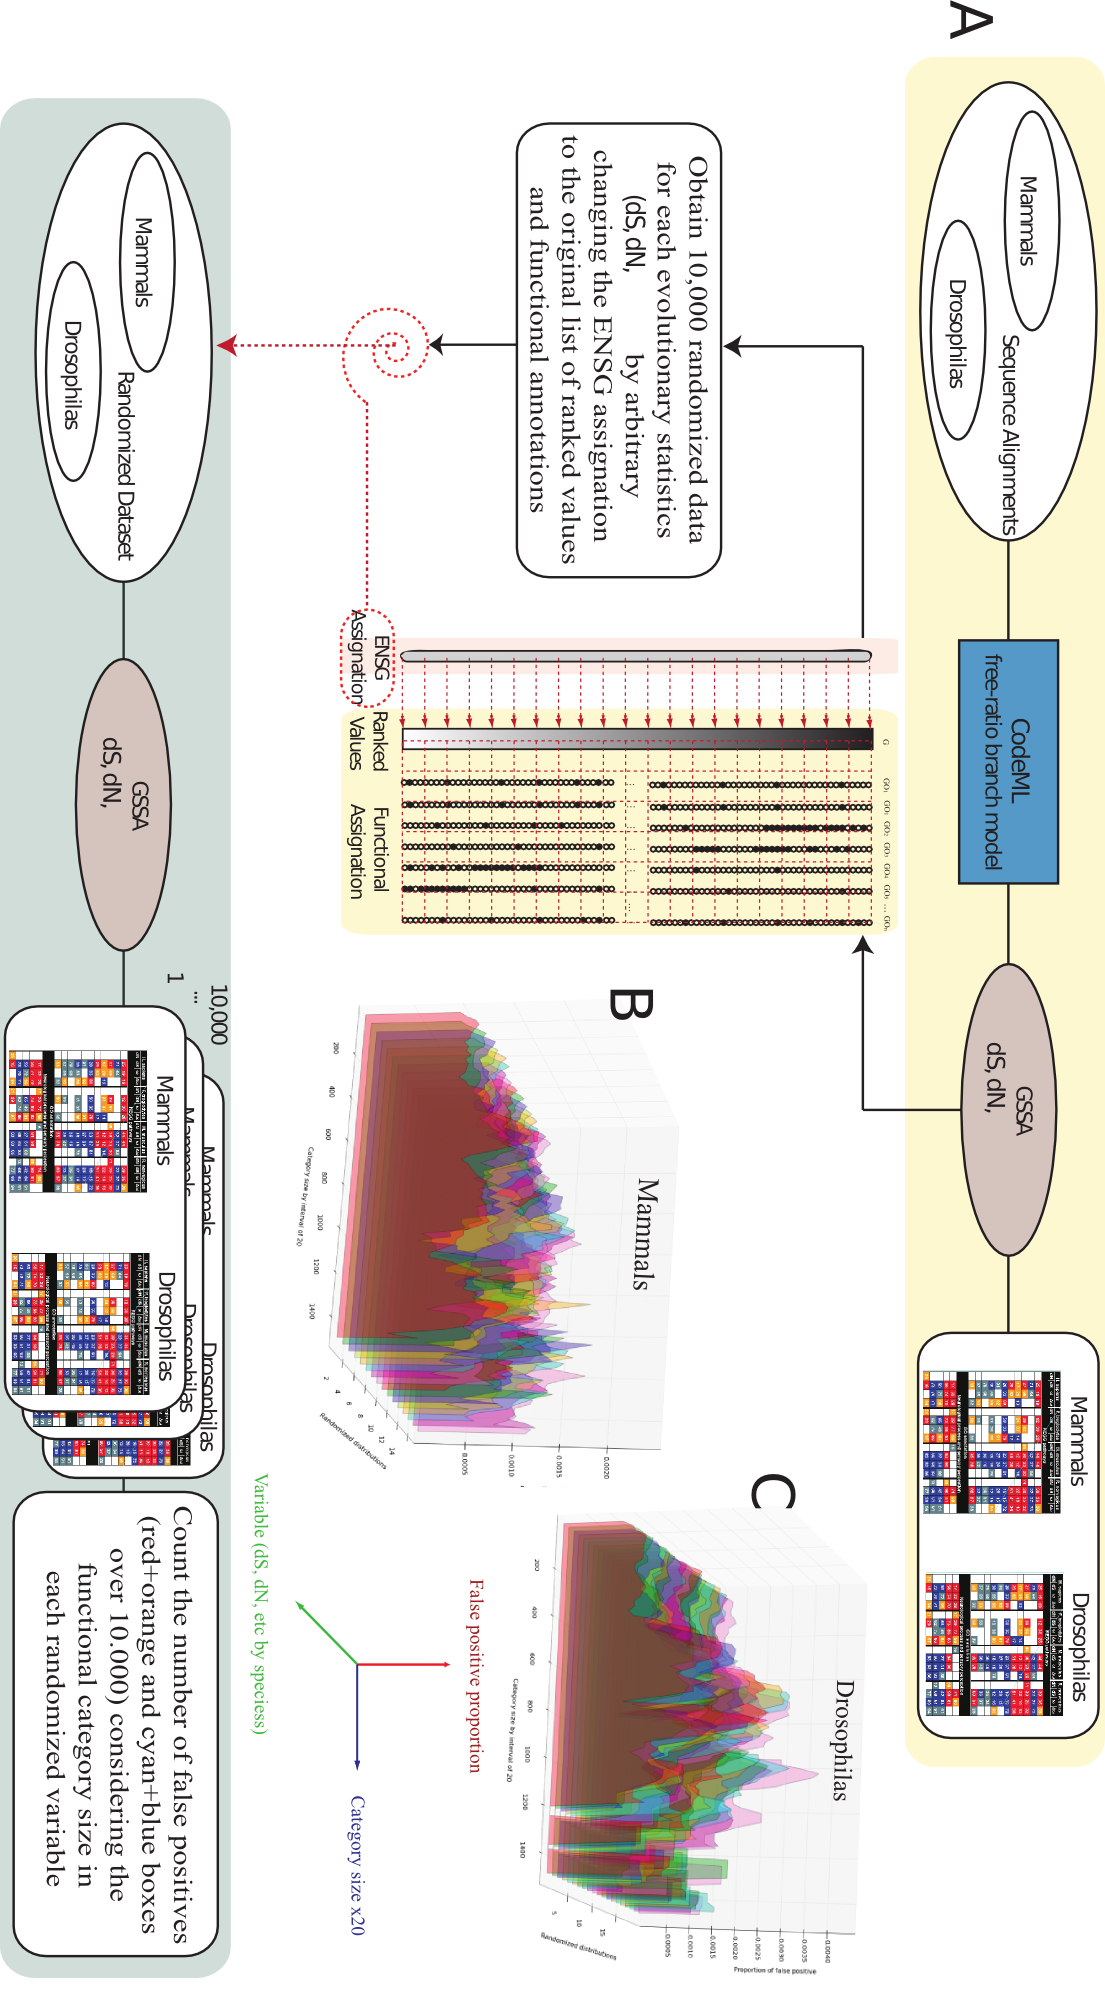
\includegraphics[height=\textheight]{tex_source/figures/gssa/gssa_simulations.png}
\caption[Randomisation experiment.]{{\bf Randomisation experiment.} \\(A) The pipeline shows the steps followed to tests possible biases attributed to the size of the functional category, the magnitude of change in evolutionary rate and the proportion of genes experiencing a rate change in the GSSA. The proportion of false positive results never reached 5\% (FDR) in mammals (B) and Drosophila (C).}
\label{fig:gssa_simul}
\end{FPfigure}

Finally, in order to validate the independence of the GSSA from the effects of alternative evolutionary constraints we simulated selective regimes (purifying selection, positive selection and relaxation of selective constraints) using branch-site models. Here we addressed the possibility of a variation in the representation of significant results after GSSA (see \fref{fig:gssa_simul_pipe}{}). The pipeline described here, shows three different areas: 
\begin{itemize}
\item \textbf{Real Data}: the dark yellow area describes the steps used to reach to results described in the manuscript. The light yellow area describes the use of the CodeML program from PAML package (reference 15 in the ms) to extract -from the original set of sequences -the evolutionary parameters to simulate new sequences under purifying selection (PF), positive selection (PS) and relaxation of the selective constraints (RX) using branch-site models (see model description below). Human, mouse, \textit{D. erecta} and \textit{D. melanogaster} were used as foreground species in the corresponding models.
\item \textbf{Simulated Data}: Evolver (PAML program) simulates sequences using parameters (codon frequencies and branch lengths) from the empirical data. We checked the desired characteristics of positive selection (PS) and relaxation of selective constraints (RX) on the set of the simulated sequences \tref{tab:psg_simul}. Evolutionary variables (dS, dN, $\omega$ and $\Delta\omega$) were estimated from simulated sequences by means of a free-ratio branch model (CodeML). The complete pipeline of the GSSA was applied in the simulated data.
\item \textbf{Testing simulation}: The odd-ratio of the values observed on the contingency table of each significant functional term after GSSA was computed. Values higher and lower than one contribute to the total number of functional modules with significant high and low $\omega$ values. To test the statistical contribution of these functional modules to these extremes on the simulated regimes (PS, RX and PF) the log odd-ratios were compared using t-test.
\end{itemize}

\begin{figure}
\centering 
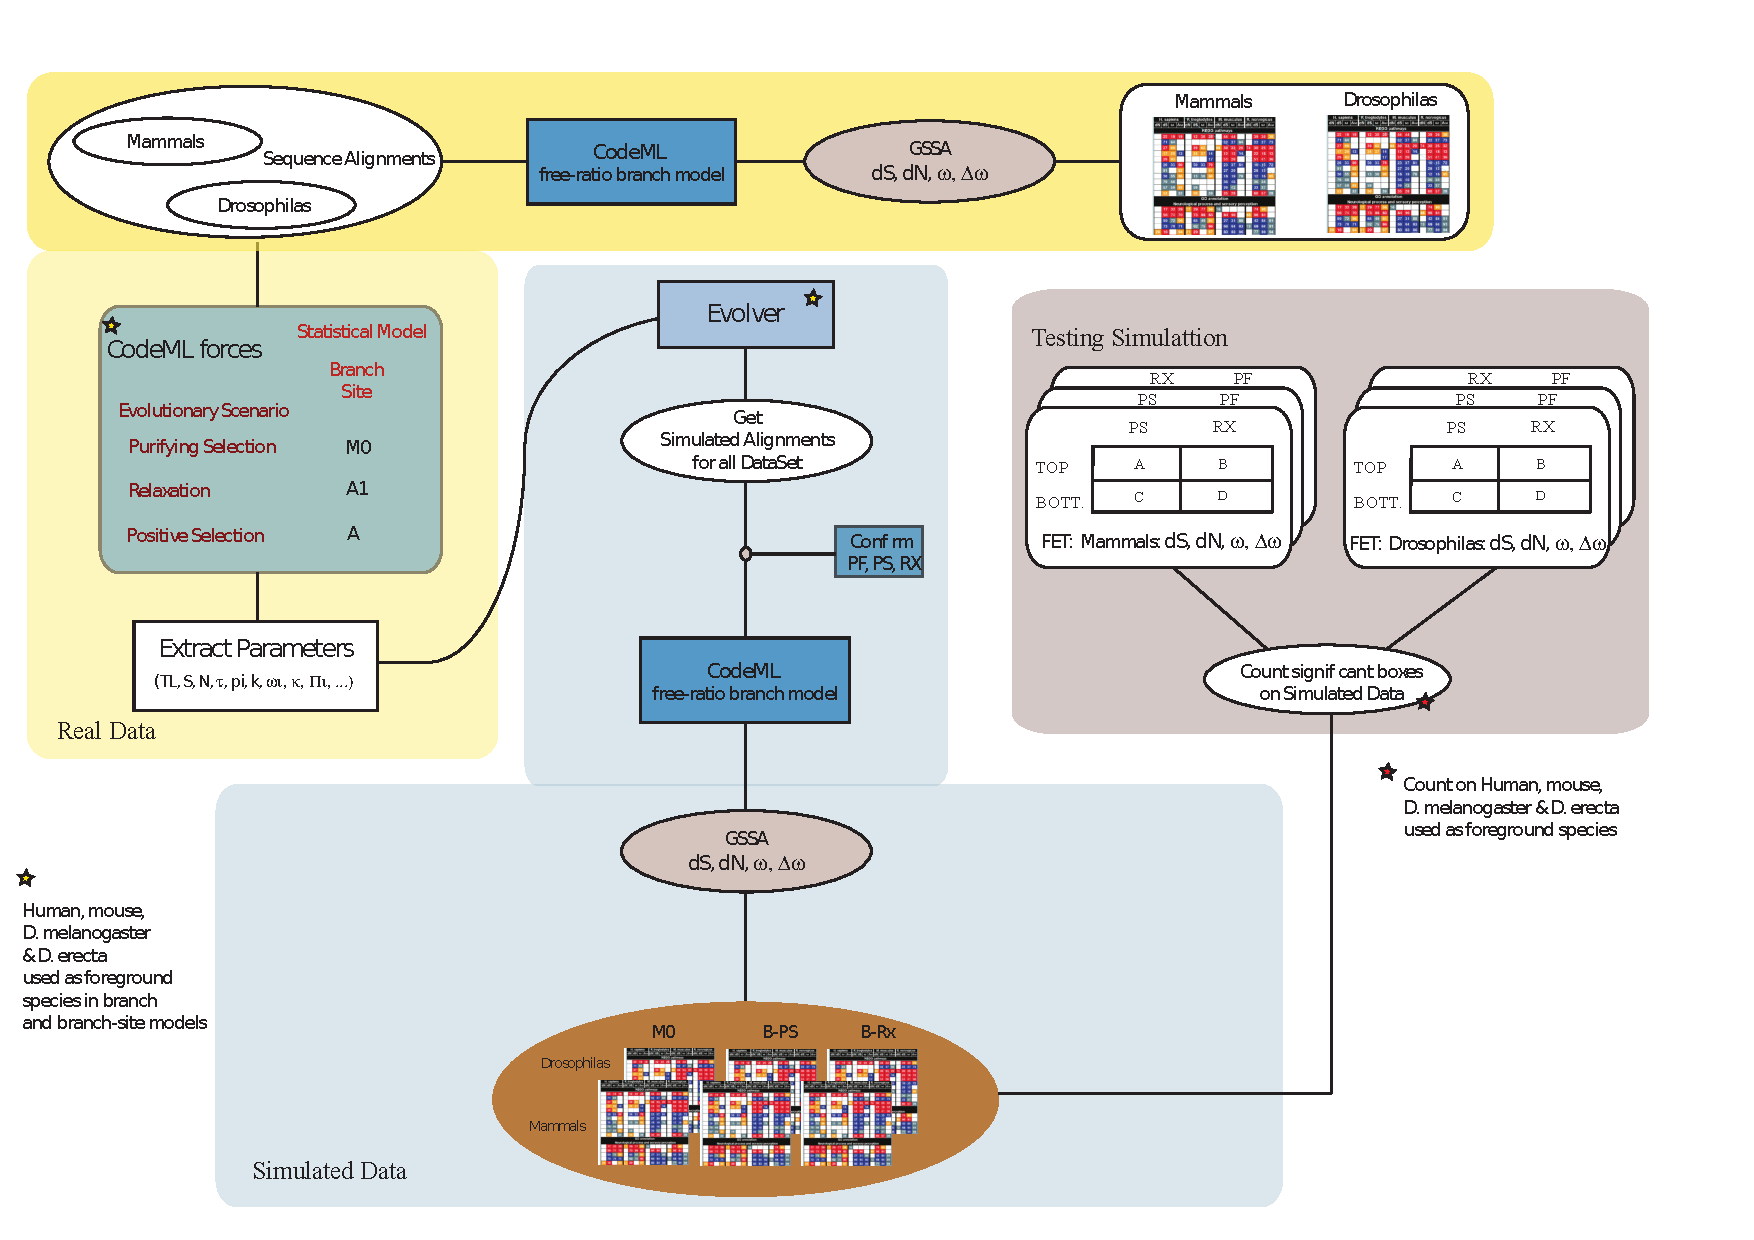
\includegraphics[width=\textwidth]{tex_source/figures/gssa/gssa_simulations_pipeline.pdf}
\caption[Evolutionary and statistical simulation of GSSA.]{{\bf Evolutionary and statistical simulation of GSSA.} \\ The pipeline shows the steps taken along three different spaces of analysis, the real data, the simulated data and the testing block. See Supplementary Results for a complete explanation of methods and results.}
\label{fig:gssa_simul_pipe}
\end{figure}

\rowcolors{1}{white}{white}
\begin{table}[htbp]
\begin{tabular}{l r r r r r r}
\multicolumn{1}{l}{} & \multicolumn{ 2}{c}{PS} & \multicolumn{ 2}{c}{RX} & \multicolumn{ 2}{c}{PF} \\ \hline
\multicolumn{1}{l}{} & \multicolumn{1}{c}{\# PSG} & \multicolumn{1}{c}{\# RXG} & \multicolumn{1}{c}{\# PSG} & \multicolumn{1}{c}{\# RXG} & \multicolumn{1}{c}{\# PSG} & \multicolumn{1}{c}{\# RXG} \\ \hline
Homo sapiens & 658 & 1640 & 11 & 1939 & 0 & 1 \\
Mus musculus & 1500 & 954 & 14 & 1565 & 1 & 0 \\
D. melanogaster & 736 & 630 & 25 & 1104 & 0 & 0 \\
D. erecta & 778 & 1292 & 26 & 1713 & 2 & 1 \\ \hline
\end{tabular}
\caption[Number of PSG and relaxed genes (RXG) in each of the simulated evolutionary scenarios]{Number of PSG and relaxed genes (RXG) in each of the simulated evolutionary scenarios.}
\label{tab:psg_simul}
\end{table}

Our results showed that in spite of the alternative evolutionary scenarios no significant differences were observed between log odd-ratios distribution (p<0.05). This result is exactly what we expected. The average effect of PF, and RX-PS is the proportional decrease and increase of the mean value of $\omega$ on sequences, respectively. This change has minor effects (if any) in the relative position of genes in the ranked list of genes of a genome. Accordingly, since no net differences were produced after ranking genes, no significant differences are expected after the t-test (PS-RX: p= 0.99, PS-PF: p= 0.45, and RX-PF: p= 0.46). The fact that basically the same number of significant results was observed in each evolutionary scenario confirmed this prediction \tref{tab:prop_signif}. We conclude that neither of the selective regimes simulated produce significant differences or biases in the GSSA of $\omega$ values.


\begin{table}[htbp]
\begin{center}
\begin{tabular}{l c c c}
\hline
 & PS & RX & PF \\ \hline
PS & --- & 92.50\% & 98.50\% \\
RX & 91.10\% & --- & 99.00\% \\
PF & 88.90\% & 90.60\% & --- \\ \hline
\end{tabular}
\end{center}
\caption[Proportion of significant functional categories that are still significant.]{Proportion of significant functional categories that are still significant (identical signs of odd-ratios) under a different evolutionary scenario.}
\label{tab:prop_signif}
\end{table}

\section{open on colocalization to not random}

%%% Local Variables: 
%%% mode: latex
%%% TeX-master: "../../master"
%%% End: 


\chapter{Tools, programs, methods}
\label{chap:tools}
%%% Local Variables: 
%%% mode: latex
%%% TeX-master: "../main"
%%% End: 

\chapter{Rethinking evolutionary pipelines.}
\label{chap:four}



\chapter{Conclusions}
\label{conclusion}
%%% Local Variables: 
%%% mode: latex
%%% TeX-master: "../main"
%%% End: 
%%% introduction.tex --- 

%% Author: garamonfok@gros
%% Version: $Id: introduction.tex,v 0.0 2011/10/09 18:39:32 garamonfok Exp$

\part{Conclusion}
\label{conclusion}



\newpage{}


%%%%%%%%%   Bibliography  %%%%%%%%%%%%%%%%%%%%%%%%%%%%%%%%%%%%%%%%%%%%%%%%%%%%%%

\clearpage
\pagenumbering{Roman}
\bibliographystyle{biblio/fransua} % serra et al 2011
% \bibliographystyle{cc} % serra et al 2011
%  [Serra et al.2011] Francois Serra, Leonardo Arbiza, Joaqu� Dopazo, and Hernan
%  Dopazo, Natural selection on functional modules, a genome-wide analysis. PLoS computa-
%  tional biology 7(3) (2011), p. e1001093.

% \bibliographystyle{apalike} % [serra et al 2011]
%  [Serra et al., 2011] Serra, F., Arbiza, L., Dopazo, J., and Dopazo, H. (2011). Natural
%  selection on functional modules, a genome-wide analysis. PLoS computational biology,
%  7(3):e1001093.

% \bibliographystyle{dcbib}  %[serra 2011]
%  [Serra2011] Fran�ois Serra, Leonardo Arbiza, Joaqu� Dopazo, and Hern�n Dopazo.
%  Natural selection on functional modules, a genome-wide analysis. PLoS com-
%  putational biology, 7(3):e1001093, Natural selection on functional modules,
%  a genome-wide analysis. ISSN 1553-7358. doi:10.1371/journal.pcbi.1001093


% \bibliographystyle{achicago}
%  [Serra et al.2011] Serra, Fran�ois, Leonardo Arbiza, Joaqu� Dopazo, and Hern�n
%  Dopazo. 2011. Natural selection on functional modules, a genome-wide analysis.
%  PLoS computational biology 7 (3): e1001093 (March).

\bibliography{biblio/bibliography}

%%%%%%%%%   Figs & Tables  %%%%%%%%%%%%%%%%%%%%%%%%%%%%%%%%%%%%%%%%%%%%%%%%%%%%%

\listoffigures
\listoftables

\end{document}



%%%%%%%%%   Bibliography  %%%%%%%%%%%%%%%%%%%%%%%%%%%%%%%%%%%%%%%%%%%%%%%%%%%%%%

\clearpage
\pagenumbering{Roman}
%\bibliographystyle{dcbib}
\bibliographystyle{biblio/fransua} % serra et al 2011
\bibliography{biblio/bibliography}

%%%%%%%%%   Figs & Tables  %%%%%%%%%%%%%%%%%%%%%%%%%%%%%%%%%%%%%%%%%%%%%%%%%%%%%

\listoffigures
\listoftables

\printglossaries

%%% appendix.tex --- 

\appendix
\chapter {RepeatMasker summary output}
\label{cha:repe-summ-outp}
\pagenumbering{Alph}
%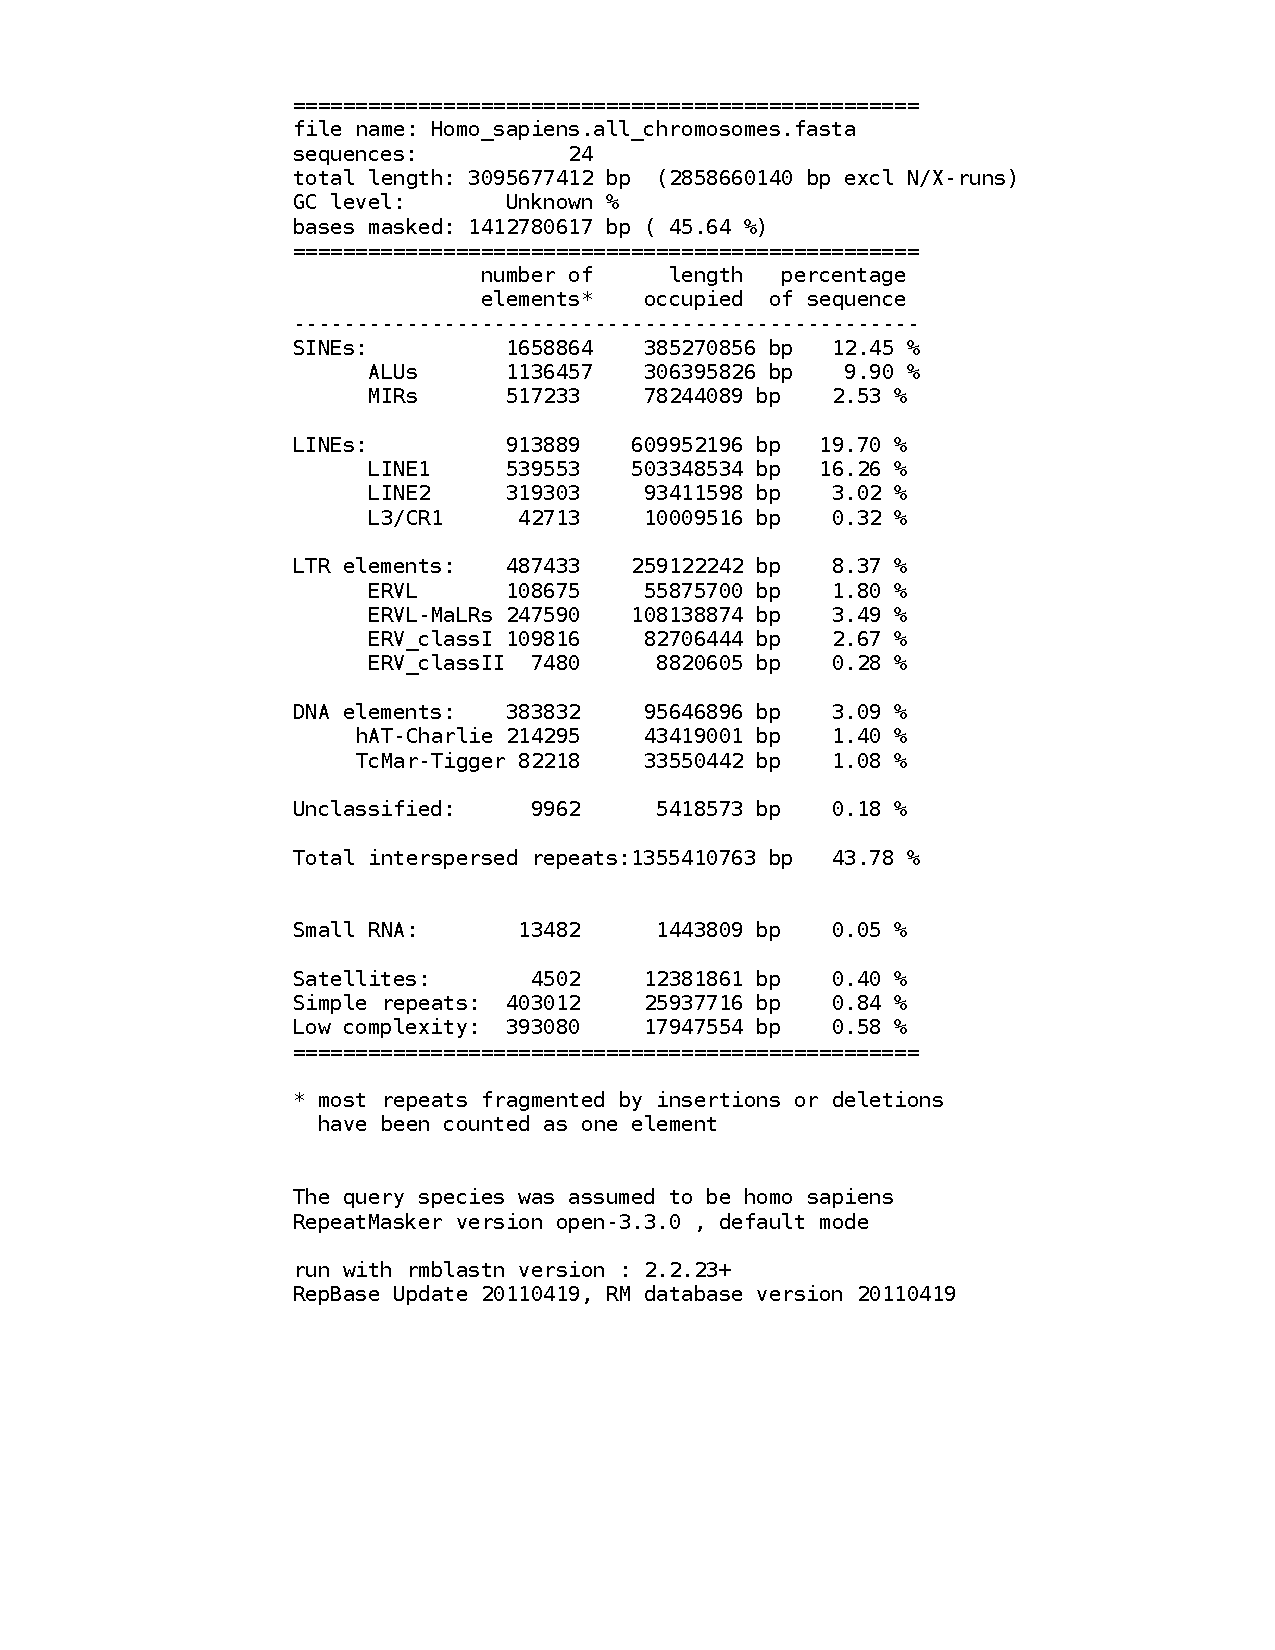
\includepdf[pages=1,addtotoc={1,section,1,Human RepeatMaser output,hsap_repmask}]{tex_source/Appendix/all_tbl.pdf}
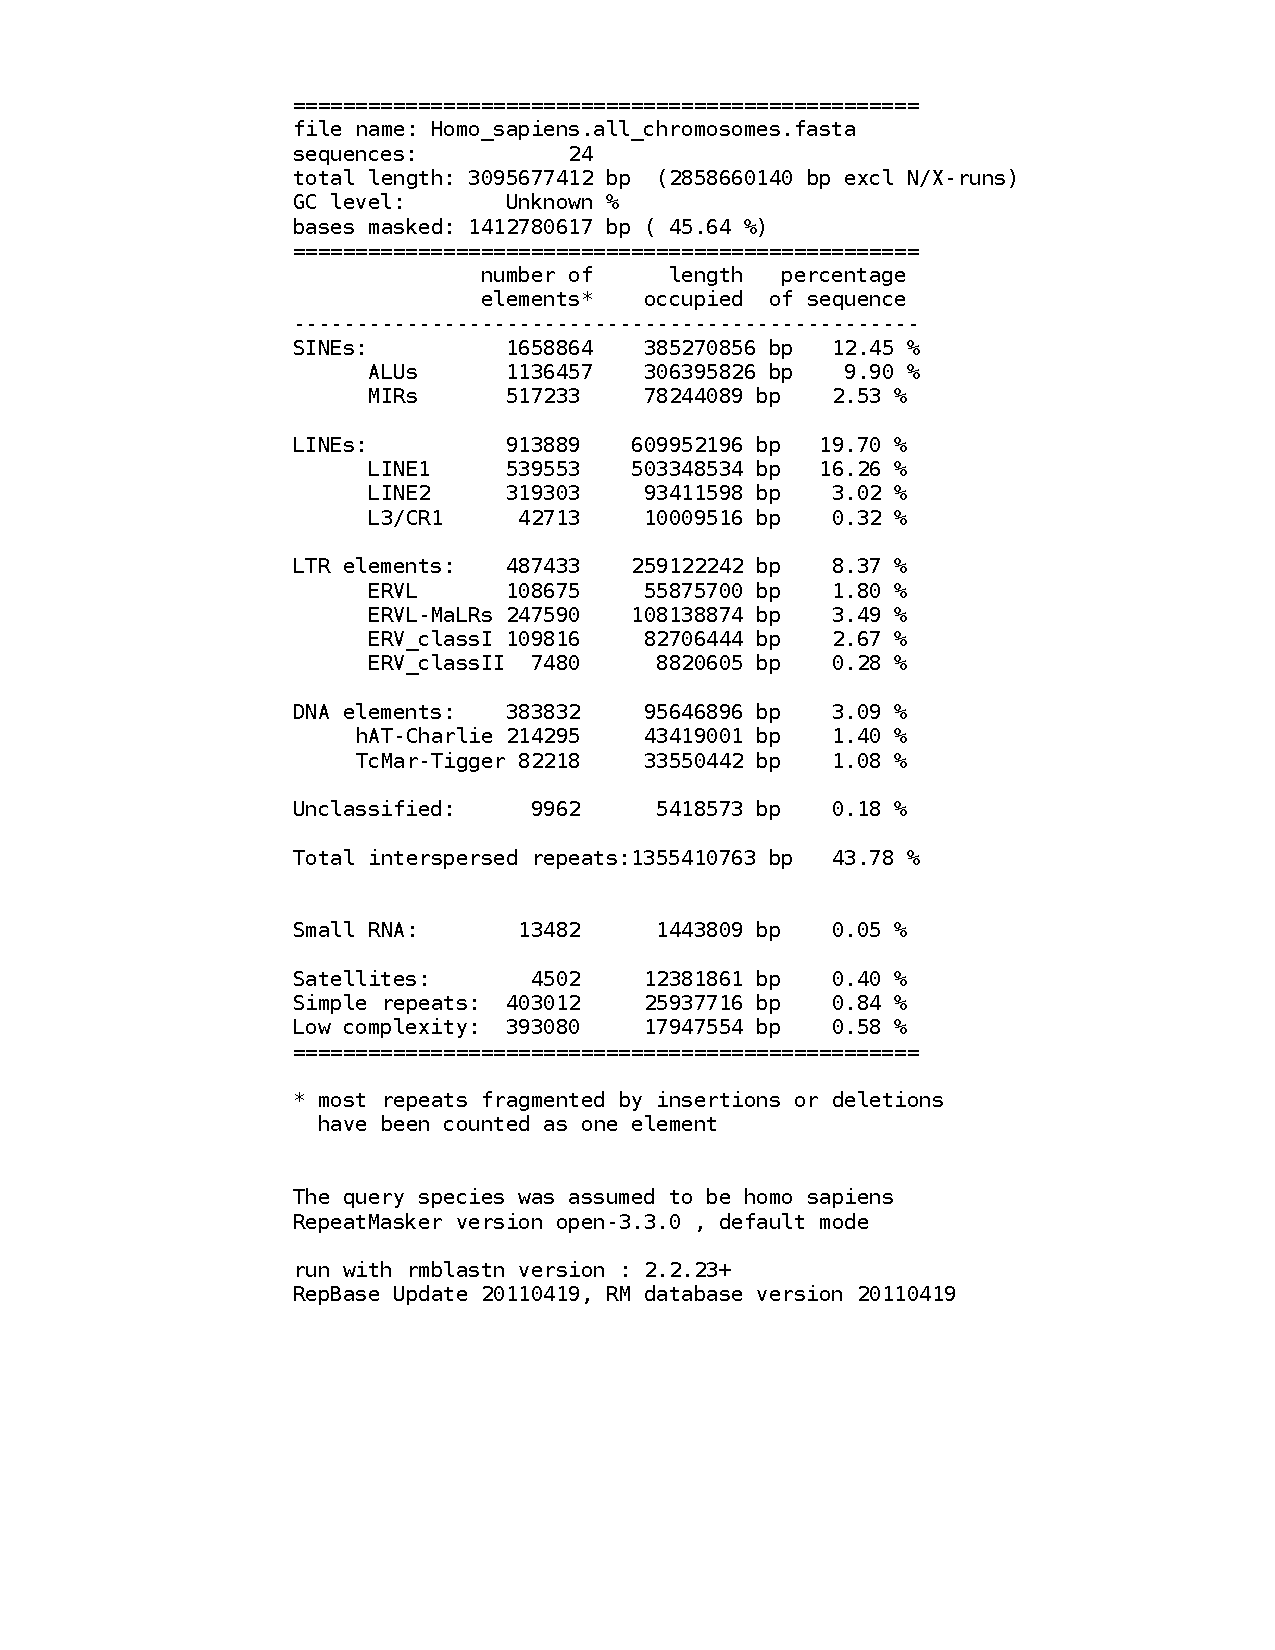
\includepdf[pages=1]{tex_source/Appendix/all_tbl.pdf}
%\pagenumbering{alph}

%%% Local Variables: 
%%% mode: latex
%%% TeX-master: "../../master"
%%% End: 



\end{document}


% \documentclass[spanish,a4paper,11pt, openany]{afthesis}
% \documentclass[spanish]{hepthesis}
% \documentclass[spanish]{muthesis}
% \documentclass[spanish]{usthesis}

%% Aesthetic spacing redefines that look nicer to me than the defaults.
% \setlength{\cftbeforepartskip}{1.5ex}
% \setlength{\cftbeforechapskip}{2.5ex}
% \setlength{\cftbeforesecskip}{0.5ex}
% German style of paragraph formatting, i.e. no indents.
% \setlength{\parskip}{1.3ex plus 0.2ex minus 0.2ex}
% \setlength{\parindent}{0pt}
% some layout    
%\usepackage{geometry}
%\geometry{tmargin=2.2cm,bmargin=2.4cm}


%\bibliographystyle{cc} % serra et al 2011
%  [Serra et al.2011] Francois Serra, Leonardo Arbiza, Joaqu� Dopazo, and Hernan
%  Dopazo, Natural selection on functional modules, a genome-wide analysis. PLoS computa-
%  tional biology 7(3) (2011), p. e1001093.

% \bibliographystyle{apalike} % [serra et al 2011]
%  [Serra et al., 2011] Serra, F., Arbiza, L., Dopazo, J., and Dopazo, H. (2011). Natural
%  selection on functional modules, a genome-wide analysis. PLoS computational biology,
%  7(3):e1001093.

% \bibliographystyle{dcbib}  %[serra 2011]
%  [Serra2011] Fran�ois Serra, Leonardo Arbiza, Joaqu� Dopazo, and Hern�n Dopazo.
%  Natural selection on functional modules, a genome-wide analysis. PLoS com-
%  putational biology, 7(3):e1001093, Natural selection on functional modules,
%  a genome-wide analysis. ISSN 1553-7358. doi:10.1371/journal.pcbi.1001093

% \bibliographystyle{achicago}
%  [Serra et al.2011] Serra, Fran�ois, Leonardo Arbiza, Joaqu� Dopazo, and Hern�n
%  Dopazo. 2011. Natural selection on functional modules, a genome-wide analysis.
%  PLoS computational biology 7 (3): e1001093 (March).





%%% Local Variables:
%%% mode: latex
%%% TeX-master: t
%%% End: 
